% Manuscript: Coordinated scheduling for consecutive demand response in AI data center integrated energy
% systems considering cross-event computing-storage recovery.
% Build: ./build.sh   (XeLaTeX; references are numbered in order of first citation by tools/order_refs.py)
\documentclass[9pt,twocolumn]{extarticle}
\usepackage{aeprep}
\graphicspath{{../matlab/figures_en/}}

%% ------------------------------------------------------------------ authors (to be completed)
\newcommand{\PaperTitle}{Coordinated scheduling for consecutive demand response in AI data center integrated energy systems considering cross-event computing--storage recovery}
\newcommand{\PaperAuthors}{First Author\,\textsuperscript{a}, Second Author\,\textsuperscript{a}, Third Author\,\textsuperscript{b}, Corresponding Author\,\textsuperscript{a,}$^{*}$}
\newcommand{\PaperAffiliations}{%
  \textsuperscript{a}\,[Department, University, City, Postcode, Country]\par
  \textsuperscript{b}\,[Department, University, City, Postcode, Country]}
\newcommand{\PaperEmail}{[e-mail address]}
\renewcommand{\RunningAuthors}{First Author et al.}
\hypersetup{pdftitle={\PaperTitle},pdfauthor={First Author et al.},
  pdfkeywords={AI data center; consecutive demand response; joint computing-storage recovery; virtual storage;
  distributionally robust optimization; integrated energy system}}

% notation shortcuts used throughout the manuscript
\newcommand{\Pg}{P^{\mathrm{G}}}
\newcommand{\Pb}{P^{\mathrm{b}}}
\newcommand{\Pcap}{\bar P}
\newcommand{\Bbar}{\bar B}
\newcommand{\pdyn}{p^{\mathrm{dyn}}}
\newcommand{\pidle}{p^{\mathrm{idle}}}
\newcommand{\Pch}{P^{\mathrm{ch}}}
\newcommand{\Pdis}{P^{\mathrm{dis}}}
\newcommand{\Qtc}{Q^{\mathrm{TC}}}
\newcommand{\Qtd}{Q^{\mathrm{TD}}}
\newcommand{\Qec}{Q^{\mathrm{EC}}}
\newcommand{\Pgt}{P^{\mathrm{GT}}}
\newcommand{\Ppv}{P^{\mathrm{PV}}}
\newcommand{\Pit}{P^{\mathrm{IT}}}
\newcommand{\crb}{c^{\mathrm{rb}}}
\newcommand{\cjct}{c^{\mathrm{jct}}}
\newcommand{\clate}{c^{\mathrm{late}}}
\newcommand{\cdeg}{c^{\mathrm{deg}}}
\newcommand{\COP}{\mathrm{COP}}
\newcommand{\lch}{\lambda^{\mathrm{ch}}}
\newcommand{\Cset}{\mathcal{C}}
\newcommand{\Tset}{\mathcal{T}}
\newcommand{\Kset}{\mathcal{K}}
\newcommand{\Iset}{\mathcal{I}}
\newcommand{\Wset}{\mathcal{W}}
\newcommand{\Hs}{H}
\newcommand{\dt}{\Delta t}
\newcommand{\ie}{i.e.}
\newcommand{\eg}{e.g.}
\newcommand{\CNY}{CNY}
\newcommand{\tenk}{$10^4$\,CNY}
\newcommand{\figref}[1]{Fig.~\ref{#1}}
\newcommand{\tabref}[1]{Table~\ref{#1}}
\newcommand{\secref}[1]{Section~\ref{#1}}
\newcommand{\appref}[1]{Appendix~\ref{#1}}
% appendix numbering of floats and equations ("Fig. A.1", "Table B.2", "(B.3)")
\newcommand{\appendixnumbering}{%
  \setcounter{figure}{0}\setcounter{table}{0}\setcounter{equation}{0}%
  \renewcommand{\thefigure}{\thesection.\arabic{figure}}%
  \renewcommand{\thetable}{\thesection.\arabic{table}}%
  \renewcommand{\theequation}{\thesection.\arabic{equation}}}
% end-of-proof square (not predefined by unicode-math)
\AtBeginDocument{\providecommand{\square}{\mdlgwhtsquare}}


\begin{document}
\thispagestyle{firstpage}
\twocolumn[{%
\begin{center}
{\fontsize{7.5}{9}\selectfont\color{aeblue} Manuscript prepared for submission to \textit{Applied Energy}}
\end{center}
\vspace{-1mm}
\aethickrule
\vspace{7mm}
{\raggedright\fontsize{15.5}{19}\selectfont \PaperTitle\par}
\vspace{4.5mm}
{\raggedright\fontsize{9.6}{12}\selectfont \PaperAuthors\par}
\vspace{2.5mm}
{\raggedright\fontsize{6.6}{8.4}\selectfont\itshape \PaperAffiliations\par}
\vspace{4mm}
\aethinrule
\vspace{3.2mm}
\spacedcaps{Highlights}\par
\vspace{1.6mm}
\aethinrule
\vspace{0.6mm}
{\fontsize{7.6}{9.6}\selectfont
\noindent$\bullet$ Cross-event joint computing--storage recovery for consecutive demand response.\par
\noindent$\bullet$ Lag-bounded backlog makes deferrable AI computing a deadline-exact virtual storage.\par
\noindent$\bullet$ Capability bound, closed-form recovery value and recovery-channel price are derived.\par
\noindent$\bullet$ Exact robust commitment MILP and plan--price distributed coordination are proposed.\par
\noindent$\bullet$ Reliable DR capacity rises by 33\% and cost falls by 2.9--4.0\% over 52 test days.\par}
\vspace{1.2mm}
\aethinrule
\vspace{5mm}
\noindent
\begin{minipage}[t]{0.245\textwidth}
\spacedcaps{Article info}\par\vspace{1.6mm}\aethinrule\vspace{1.2mm}
{\fontsize{6.8}{8.6}\selectfont\raggedright
\textit{Keywords:}\par
AI data center\par
Consecutive demand response\par
Joint computing--storage recovery\par
Virtual storage\par
Distributionally robust optimization\par
Integrated energy system\par}
\end{minipage}\hfill
\begin{minipage}[t]{0.725\textwidth}
\spacedcaps{Abstract}\par\vspace{1.6mm}\aethinrule\vspace{1.2mm}
{\fontsize{7.6}{9.75}\selectfont\justifying
With the rapid growth of artificial intelligence (AI) computing, AI data centers are increasingly called on for demand
response (DR). However, DR events often come consecutively within one evening peak: each event leaves deferred computing
work and depleted storage, and both must be recovered in short inter-event gaps through the same connection-limited grid
headroom, which erodes the capability of later events. This study develops a coordinated scheduling method for
consecutive DR in AI data center integrated energy systems that jointly optimizes cross-event computing and storage
recovery. Tiered service-level agreements are modelled by lag-bounded backlog constraints, which are proved equivalent to
deadline-feasible earliest-deadline-first execution, so that deferrable computing acts as a virtual storage that competes
with battery and chilled-water storage for one recovery channel. An upper bound on the next event's capability, a
closed-form value of joint recovery, a single recovery-channel price, the convex capability region of commitment vectors
and an exact mixed-integer linear reformulation of the distributionally robust commitment are derived. A day-ahead
commitment--intraday rolling framework embedding the Jiangsu DR rules is established, together with a distributed variant
that exchanges only power plans and prices. Case studies on a 16,000-GPU data center built from public workload traces
and ERA5 weather show that, compared with the strongest tuned and price-coordinated independent-recovery benchmarks,
joint recovery keeps all events valid on all 52 test days and reduces the total cost by 2.9--4.0\%. It raises the
reliably deliverable capacity from 6 to 8~MW per event, which is equivalent to about 9--12~MWh of battery or 2.9~MW of
connection capacity, whereas independent recovery shrinks the cross-event energy budget by about 18\%. When the IT
scheduler and the facility controller exchange only power plans and prices, three exchanges per 15-min step recover 85\%
of the cost advantage of joint recovery. The proposed method improves the reliability and economy of consecutive DR and
supports the grid-interactive operation of AI data centers.\par}
\vspace{1.4mm}\aethinrule
\end{minipage}
\vspace{6mm}
}]
{\renewcommand{\thefootnote}{\fnsymbol{footnote}}\footnotetext[1]{Corresponding author.\ \textit{E-mail address:} \PaperEmail.}}

% boxed nomenclature (full width, top of page 2)
\begin{figure*}[!t]
\setlength{\fboxsep}{6pt}\setlength{\fboxrule}{0.5pt}
\fbox{\begin{minipage}{\dimexpr\textwidth-2\fboxsep-2\fboxrule\relax}
\fontsize{6.9}{8.45}\selectfont
\noindent\textbf{\normalsize Nomenclature}\par\vspace{2pt}
\setlength{\columnsep}{7mm}
\begin{multicols}{2}
\setlength{\nomsymw}{15mm}
\nomhead{Abbreviations}
\nom{AI(DC)}{Artificial intelligence (AI data center)}
\nom{IES}{Integrated energy system}
\nom{DR}{Demand response}
\nom{SLA}{Service-level agreement}
\nom{EDF}{Earliest deadline first}
\nom{BESS}{Battery energy storage system}
\nom{TES}{Chilled-water thermal energy storage}
\nom{COP}{Coefficient of performance}
\nom{TOU}{Time-of-use (tariff)}
\nom{PV}{Photovoltaic}
\nom{MPC}{Model predictive control}
\nom{(MI)LP}{(Mixed-integer) linear programme}
\nom{SP, RO}{Stochastic programming, (scenario-)robust optimization}
\nom{DRO}{Distributionally robust optimization}
\nom{CVaR}{Conditional value-at-risk}
\nom{ADMM}{Alternating direction method of multipliers}
\nom{PUE}{Power usage effectiveness}
\nom{JR, IR}{Joint recovery, independent recovery}
\nom{IR-R}{Rule-based independent recovery}
\nom{IR-O, IR-O*}{Sequentially optimized IR with a fixed / tuned split}
\nom{IR-P}{IR coordinated by a one-shot channel price}
\nom{JR-M}{Event-by-event (myopic) joint recovery}
\nom{JR-D, JR-S}{Joint recovery by deterministic / scenario MPC}
\nom{JR-A}{Distributed joint recovery by plan--price exchange}
\nomhead{Sets and indices}
\nom{$t\in\Tset$, $\dt$}{Time steps (00:00 of day D to 06:00 of day D+1, 120 steps); step length 0.25~h}
\nom{$c\in\{1,2,3\}$}{Classes of deferrable jobs (short, medium, long)}
\nom{$k\in\Kset$}{DR events; $\Tset_k=[s_k,e_k]$ event steps, $D_k$ duration}
\nom{$\Iset_k$, $\Wset_k$}{Gap between events $k$ and $k+1$; 2-h rebound window after event $k$}
\nom{$\omega\in\Omega$, $\hat p_\omega$}{Day-ahead scenarios and their empirical probabilities}
\nomhead{Parameters}
\nom{$N$}{Number of GPUs (16,000)}
\nom{$\pidle$, $\pdyn$}{Idle and dynamic power per GPU (0.26, 0.79~kW)}
\nom{$G^{\mathrm{inf}}_t$, $G^{\mathrm{fix}}_t$}{GPUs busy with online inference and non-deferrable training}
\nom{$\kappa^{\mathrm{inf}}$}{Dynamic-power factor of inference GPUs (0.65)}
\nom{$a_{c,t}$}{Nominal work of class $c$ arriving in step $t$ (GPU$\cdot$h)}
\nom{$L_c$}{Lag bound (deadline) of class $c$ (0.5/1.5/3~h)}
\nom{$\Bbar_{c,t}$}{Deadline-implied backlog bound = virtual-storage capacity (GPU$\cdot$h)}
\nom{$a^{\mathrm{aux}}$, $\theta$}{Distribution/air-handling loss factor; heat per unit IT power}
\nom{$\COP_t$}{COP of the electric chiller plant (temperature dependent)}
\nom{$\varepsilon_t$}{Facility electricity per GPU$\cdot$h of work, $(1+a^{\mathrm{aux}}+\theta/\COP_t)\pdyn$}
\nom{$\Pcap$, $\hat P$, $\gamma$}{Connection limit $\Pcap=\gamma\hat P$; typical-day peak import; margin}
\nom{$\Pb_t$}{DR baseline (mean of the five previous workdays)}
\nom{$\pi_t$, $\pi_k$}{TOU price; DR payment rate of event $k$}
\nom{$\kappa$}{Shortfall coefficient (shortfall assessed at $\kappa\pi_k$)}
\nom{$\crb$, $c^{\mathrm{pre}}$}{Rebound charge; optional pre-event load-up charge}
\nom{$\cjct$, $\clate$}{Job-delay cost; overdue penalty (CNY per GPU$\cdot$h and hour)}
\nom{$\bar P^{\mathrm{B}}$, $E^{\min/\max}$}{BESS power and energy limits}
\nom{$\eta_{\mathrm{c}}$, $\eta_{\mathrm{d}}$, $\cdeg$}{BESS charge/discharge efficiency; degradation cost}
\nom{$\bar Q^{\mathrm{S}}$, $S^{\min/\max}$}{TES power and capacity limits; $\eta^{\mathrm{TC}},\eta^{\mathrm{TD}}$ efficiencies}
\nom{$\bar P^{\mathrm{GT}}$, $\eta_{\mathrm{e}}$, $\eta_{\mathrm{h}}$}{Gas-engine capacity, electrical and heat-recovery efficiency}
\nom{$\COP^{\mathrm{AC}}$}{COP of the absorption chiller}
\nom{$\delta$}{Radius of the $\ell_1$ ambiguity set of the day-ahead DRO}
\nom{$\rho$}{Penalty parameter of the plan--price iteration (ADMM)}
\nom{$\tau_c$}{Gang-weighted mean run time of class $c$ (rigid-job bound)}
\nom{$o_c$}{Pause/resume overhead per newly paused GPU (GPU$\cdot$h)}
\nomhead{Variables}
\nom{$y_{c,t}$}{GPUs executing deferrable class $c$}
\nom{$B_{c,t}$, $v_{c,t}$}{Backlog (computing recovery state, GPU$\cdot$h); overdue work}
\nom{$\zeta_{c,t}$, $w_{c,t}$}{Capped dynamic power (GPU equivalents); throughput loss}
\nom{$u_{c,t}$}{GPUs newly paused relative to the nominal load}
\nom{$\Pg_t$}{Grid import}
\nom{$\Pch_t$, $\Pdis_t$, $E_t$}{BESS charging, discharging power and energy}
\nom{$\Qtc_t$, $\Qtd_t$, $S_t$}{TES charging, discharging and stored cooling}
\nom{$\Pgt_t$, $Q^{\mathrm{rec}}_t$}{Gas-engine output; recovered heat sent to the absorption chiller}
\nom{$\Qec_t$, $\Ppv_t$}{Electric-chiller cooling; PV power used}
\nom{$\Theta_t$}{Stored heat of the data hall (optional thermal inertia)}
\nom{$P^{\mathrm{HP}}_t$, $E^{\mathrm{HW}}_t$}{Heat-pump power; hot-water tank level (optional)}
\nom{$C_k$}{Committed reduction of event $k$ (day-ahead decision)}
\nom{$\bar r_k$, $z_k$}{Mean reduction of event $k$; validity binary}
\nom{$R_k$, $s_k$, $\Delta^{\mathrm{rb}}_k$}{Paid reduction; shortfall; peak rebound above baseline}
\nom{$H$}{Recovery-channel energy available in a gap}
\nom{$\lambda_t$, $\nu_t$, $\mu_{c,t}$}{Channel price; marginal value of stored energy; marginal cost of backlog}
\end{multicols}
\end{minipage}}
\end{figure*}

\section{Introduction}
\label{sec:intro}

The rapid expansion of artificial intelligence (AI) is turning data centers into one of the fastest-growing
electricity loads. The International Energy Agency estimates that data centers consumed about 415~TWh in 2024, roughly
1.5\% of global electricity use, and that their demand may reach about 945~TWh by 2030~\cite{iea2025}. In the United
States their share already reached 4.4\% in 2023 and may rise to 325--580~TWh by 2028~\cite{shehabi2024}, while China
requires new large data centers to achieve a power usage effectiveness (PUE) of 1.25 or lower~\cite{ndrc2024dc}.
Because new AI campuses are increasingly limited by grid interconnection rather than by chips, operational flexibility
is becoming a condition of connection: curtailing large flexible loads for 0.25--1\% of the hours could accommodate
76--126~GW of additional load in 22 balancing authorities of the United States~\cite{norris2025}, the flexibility of AI loads can reduce grid
investment and operating costs by 3--21\%~\cite{chen2026defer}, and the Texas Senate Bill~6 links the interconnection of
large loads to curtailment obligations during grid emergencies~\cite{texas2025sb6}. Power-flexible AI data centers are
therefore regarded as a new class of grid-responsive resources~\cite{williams2026}, and a field demonstration in Phoenix
reduced the power of a 256-GPU cluster by 25\% for three hours~\cite{colangelo2025}. In China, demand-side regulations
require a demand response (DR) capability of 3--5\% of the maximum load~\cite{ndrc2023dsm}. Under the Jiangsu DR rules,
an event is valid only if the mean load falls by at least 80\% of the confirmed reduction, payments are capped at
120\% of it, agreed responses are limited to two calls and 2~h per day, and fast responses with short notice are paid up to 1.6 times
the base rate~\cite{jiangsu2024dr}. One evening peak can therefore trigger several events that are separated by gaps of
an hour or less, and an AI data center that responds to the first event must be ready for the next one shortly
afterwards.

In the area of data center DR and AI workload flexibility, early studies showed that data centers can avoid coincident
peaks by shifting deferrable workloads and using local generation~\cite{liu2013}, discussed the opportunities and
challenges of data center DR~\cite{wierman2014}, and reviewed how Internet data centers participate in DR
programs~\cite{chen2020review}. Carbon-aware computing shifts flexible workloads towards low-carbon hours at fleet
scale~\cite{radovanovic2023}. For AI workloads, simulation studies estimate a power flexibility of 18--55\% for AI data
centers~\cite{acun2026}, power capping and frequency scaling provide additional levers for large language model (LLM)
workloads~\cite{patel2024}, and quantization can turn LLM inference into a DR resource~\cite{du2026}. Agreements that
curtail machine-learning workloads during grid stress have also been signed in practice~\cite{google2025}. However, a
study of 185 days of production traces from 155,000 GPUs found that a scalar flexibility ratio overstates the dependable
load relief by 17--47\%~\cite{li2026scalar}, and synchronous training causes large power swings~\cite{choukse2025}.
These studies characterise how much an AI data center can reduce in a single event, but they do not consider how the
recovery needs left by one event constrain the next event.

In the area of data center integrated energy systems (IES), multi-level DR dispatch of data centers with district
autonomy~\cite{han2024}, exergy-based planning and operation of computing-power IES~\cite{lin2025} and the operation
of data centers with combined cooling, heating and power (CCHP) and spatio-temporally adjustable loads~\cite{fan2026}
have been studied. Zhang et al.~\cite{zhang2026bilevel} proposed a bi-level distributionally robust planning model for
data center clusters in which time-shiftable and space-transferable loads act as virtual energy storage, and the reuse of
data center waste heat in district heating has been reviewed~\cite{huang2020,wahlroos2018}. In these models, deferred
workloads are bounded by constant virtual-queue limits and recovered by their own rules, while storage is recharged by
the energy system, so the recovery of computing backlog and that of storage are treated as separate subproblems. As
shown in \secref{sec:computing}, a constant queue limit cannot guarantee that every task meets its deadline when
arrivals are low and is unnecessarily conservative when arrivals are high.

In the area of recovery and coordination, Evans et al.~\cite{evans2022} proposed a flexibility framework with recovery
guarantees for aggregated energy storage, in which discharge and recovery are coupled and the recovery capability is
summarised by a single virtual battery; virtual-battery models also describe the aggregate flexibility of
thermostatically controlled loads~\cite{hao2015}. Load payback after DR events is a common side effect of
DR~\cite{wrinch2012}, and the choice of the customer baseline affects the settled reduction~\cite{chao2011}.
Uncertainty in DR scheduling is usually handled by scenario-based stochastic model predictive control
(MPC)~\cite{schildbach2014} or by distributionally robust optimization (DRO), which in two-stage problems is typically
solved by duality-based reformulation and column-and-constraint generation~\cite{zhang2026bilevel,zeng2013,esfahani2018}.
Coordination between the IT scheduler and the facility energy management system is commonly realised by price signals,
whereas iterative schemes such as the alternating direction method of multipliers (ADMM)~\cite{boyd2011} exchange both
plans and prices. However, existing approaches consider either one homogeneous storage state or a single event, and
none addresses two heterogeneous recovery states, a deadline-bounded and nearly lossless computing backlog and a lossy
physical storage, that compete for one connection-limited recovery channel across consecutive events.

Despite substantial progress in data center DR, IES operation and storage recovery, several research gaps remain.
First, existing studies optimise a single event or treat events independently, so the state coupling between
consecutive events, \ie\ the computing backlog and the storage deficit that must be recovered through the same
connection headroom, is not modelled, and the resulting loss of deliverable capability is unknown. Second, computing
backlog and storage are recovered by separate rules or coordinated by static prices, whereas their joint value, the
conditions under which this value vanishes and the price that would coordinate them have not been characterised.
Third, commitments are assessed event by event and against weak benchmarks, without a description of the set of
deliverable commitment vectors, out-of-sample validation over many operating days, or a job-level verification of the
fluid workload model. Consequently, a scheduling framework that jointly recovers computing and storage across events,
from the day-ahead commitment to intraday operation, is still lacking.

To address these gaps, this paper proposes a coordinated scheduling method for consecutive DR in AI data center IES
(AIDC-IES) considering cross-event computing--storage recovery. The main contributions are summarised as follows.
\begin{enumerate}[label=(\arabic*),leftmargin=1.9em,itemsep=1.5pt]
\item A multi-state recovery model of computing and storage is established. Tiered service-level agreements (SLAs) are
represented by lag-bounded backlog constraints, which are proved to be exactly equivalent to deadline-feasible
earliest-deadline-first (EDF) execution (Lemma~\ref{lem:edf}), so that deferrable computing becomes a virtual storage
whose capacity is set by deadlines. Together with the battery, the chilled-water storage, the gas engine with
absorption cooling and the connection limit, the model captures how catch-up computing, recharging and the next
event's capability interact; data hall thermal inertia, waste-heat recovery, GPU power capping, pause overheads and a
rigid-job recovery bound are included as options.
\item Theoretical properties of cross-event recovery are derived: an upper bound on the deliverable capability of the
next event (Proposition~\ref{prop:bound}), a closed-form value of joint recovery and of the minimum recovery interval
(Theorem~\ref{thm:closed}), a single recovery-channel price with equal marginal values
(Proposition~\ref{prop:price}), an exact mixed-integer linear reformulation of the distributionally robust commitment
(Proposition~\ref{prop:dro}), the convex capability region of commitment vectors with a virtual-battery description
and a vertex certificate (Proposition~\ref{prop:region}), and a distributed plan--price iteration that converges to
joint recovery and recovers the channel price (Proposition~\ref{prop:admm}).
\item A day-ahead coupled commitment and intraday rolling joint-recovery framework is developed
(Algorithm~1, \tabref{tab:algorithm}). It embeds the Jiangsu settlement rules, handles uncertain event calls by
scenario trees, and admits a distributed implementation in which the IT scheduler and the facility controller keep their
own models and exchange only power plans and prices.
\item A comprehensive evaluation against strong benchmarks is conducted on a 16,000-GPU case built from public
traces. The benchmarks include independent recovery with a back-tested split, independent recovery coordinated by the
channel price of the joint plan and event-by-event joint recovery. The evaluation covers 52 out-of-sample operating
days with paired tests, risk-averse commitments, the capability region, job-level replay of all schedules and
extensions to green-power direct supply and winter waste-heat recovery, and it quantifies the reliably deliverable
capacity, its equivalent in battery and connection capacity, and the conditions under which joint recovery loses its
value.
\end{enumerate}

\section{System architecture and cross-event recovery framework}
\label{sec:system}

\subsection{Physical architecture of the system}
\label{sec:architecture}

The AI data center integrated energy system (AIDC-IES) considered in this paper is shown in \figref{fig:arch}. It
hosts $N=16{,}000$ H100-class GPUs in 2,000 eight-GPU nodes and is supplied by the utility grid through a connection
limited to $\Pcap=\gamma\hat P$, where $\hat P$ is the peak import on a typical day and $\gamma$ is the connection
margin. On site, an 8-MWp photovoltaic (PV) array, a 3-MW gas engine whose waste heat drives an absorption chiller,
temperature-dependent electric chillers, a 10-MWh chilled-water thermal energy storage (TES) and a 6-MW/12-MWh battery
energy storage system (BESS) form an electricity--cooling--heat coupled energy system. The information layer consists of
the grid operator or aggregator, which issues DR events under the Jiangsu rules~\cite{jiangsu2024dr}, the day-ahead
commitment, the intraday rolling joint-recovery controller and the execution and settlement layer.

\begin{figure*}[!t]
\centering
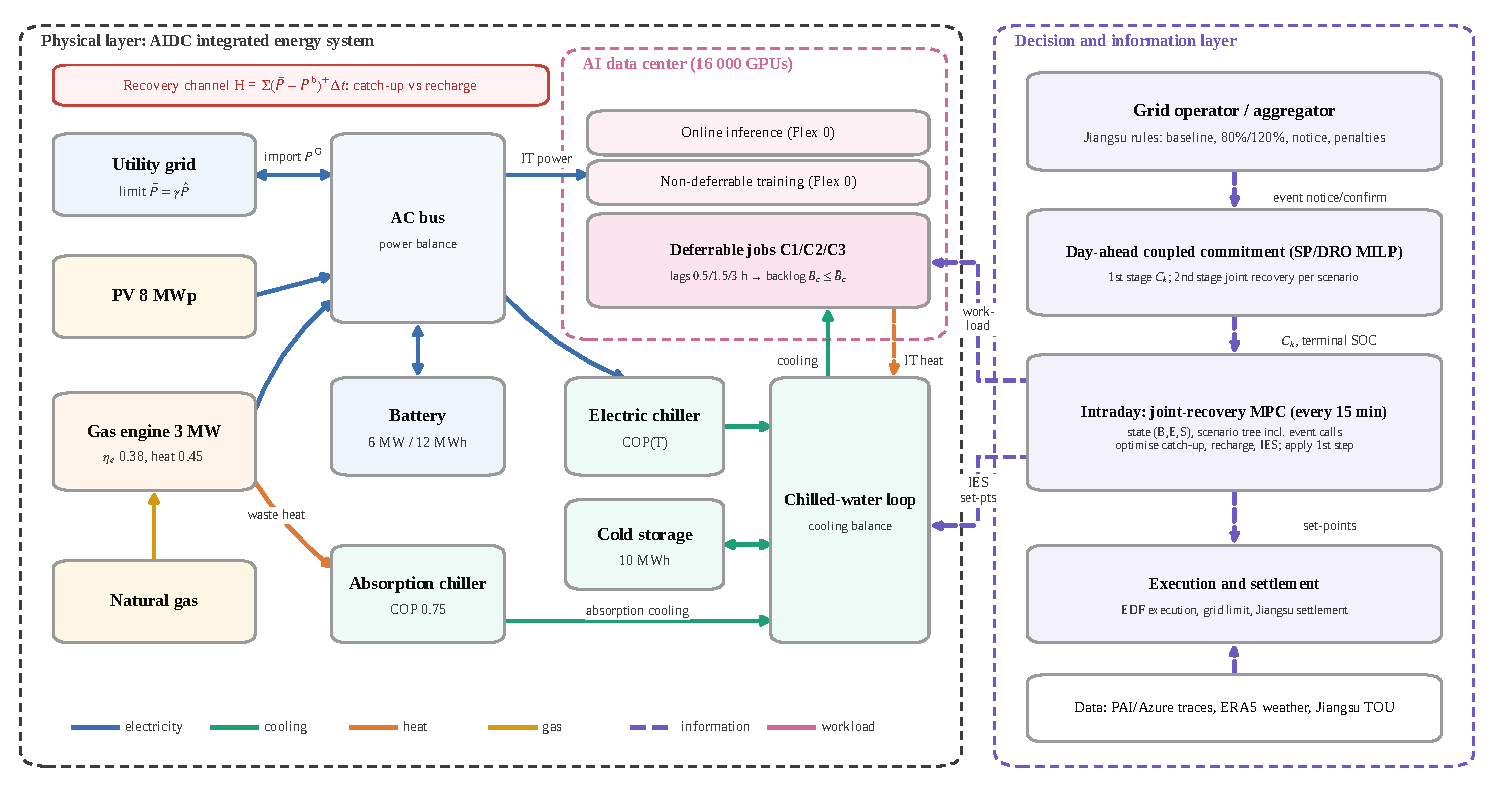
\includegraphics[width=0.98\textwidth]{fig00_architecture.pdf}
\caption{Physical and information architecture of the AI data center integrated energy system (AIDC-IES). The
recovery channel is the connection headroom above the DR baseline that is shared by catch-up computing and storage
recharging between events.}
\label{fig:arch}
\end{figure*}

The GPU workload is divided into tiers that follow the flexibility levels used in AI data center DR
programs~\cite{colangelo2025} (\tabref{tab:tiers}). Online inference, whose shape follows the Azure LLM inference
trace~\cite{stojkovic2025}, and the non-deferrable part of training are served immediately. Deferrable training and
batch jobs from the Alibaba PAI GPU trace~\cite{weng2022} are split by run time into short, medium and long classes
with lag bounds $L_c$ of 0.5, 1.5 and 3~h, \ie\ every unit of work must be completed within $L_c$ of its nominal
completion time.

\begin{table}[!t]
\caption{Workload tiers of the AI data center.}
\label{tab:tiers}
\centering\footnotesize
\begin{tabular}{@{}llll@{}}
\toprule
Tier & Source & Deferrable & Lag bound $L_c$\\
\midrule
Online inference & Azure LLM 2024~\cite{stojkovic2025} & No (Flex 0) & 0\\
Non-deferrable training & PAI $\times$ 25\%~\cite{weng2022} & No (Flex 0) & 0\\
C1 short jobs ($\le$1 h) & PAI $\times$ 75\% & Flex 1 & 0.5 h\\
C2 medium jobs (1--12 h) & PAI $\times$ 75\% & Flex 2 & 1.5 h\\
C3 long training ($>$12 h) & PAI $\times$ 75\% & Flex 3 & 3 h\\
\bottomrule
\end{tabular}
\end{table}

\subsection{Consecutive DR events and the recovery channel}
\label{sec:channel}

Three events are called on the case day. E1 (17:00--18:00) and E2 (19:00--20:00) are day-ahead agreed responses paid
3~CNY/kWh; E3 (21:00--22:00) is a fast peak-avoidance response that is pre-announced the day before and confirmed 3~h
ahead (speed coefficient 1.4, 4.2~CNY/kWh). In the uncertain variant, E3 is only announced as a possible event that is
called with probability 0.6 and confirmed or cancelled 1~h ahead (coefficient 1.6, 4.8~CNY/kWh).

Each event leaves a recovery state $\mathbf{x}_{e_k}=(B_1,B_2,B_3,E,S)$: the backlog of the three job classes and the
energy of the BESS and TES. The paper refers to the computing and storage sides as two kinds of recovery states; the
state vector has five dimensions, and one more each when data hall thermal inertia or a hot-water tank is modelled.
During the gap $\Iset_k$ between two events, catch-up computing and storage recharging draw on the same recovery
channel, whose energy is
\begin{equation}
H_k=\sum_{t\in\Iset_k}\big(\Pcap-\Pb_t\big)^+\dt ,
\label{eq:channel}
\end{equation}
minus the part that is charged as rebound in the post-event window. Catch-up computing and recharging compete for $H_k$
subject to the idle GPU capacity, the storage power limits and the job deadlines. Under independent recovery (IR) each
side recovers by its own rule or optimizer; under joint recovery (JR) the channel is allocated to the states that the
remaining events need most.

\subsection{Computing side: IT power and lag-bounded backlog}
\label{sec:computing}

With $\dt=0.25$~h and a window from 00:00 of day D to 06:00 of day D+1 (120 steps), the IT power follows the
idle-plus-dynamic model~\cite{fan2007}
\begin{equation}
\Pit_t=N\pidle+P^{\mathrm{oth}}+\pdyn\Big(\kappa^{\mathrm{inf}}G^{\mathrm{inf}}_t+G^{\mathrm{fix}}_t+\sum_{c}\big(y_{c,t}-\zeta_{c,t}\big)\Big),
\label{eq:pit}
\end{equation}
where $P^{\mathrm{oth}}=0.6$~MW is the storage and network IT power, $\kappa^{\mathrm{inf}}=0.65$ reflects that
inference GPUs seldom reach their thermal design power~\cite{patel2024}, and $\zeta_{c,t}$ is the dynamic power removed
by optional power capping (zero in the base case). The deferrable classes share the free GPU capacity,
\begin{equation}
\sum_c y_{c,t}\le u^{\max}N-G^{\mathrm{inf}}_t-G^{\mathrm{fix}}_t ,
\label{eq:gpucap}
\end{equation}
with $u^{\max}=0.95$, and their backlog evolves as
\begin{equation}
B_{c,t}=B_{c,t-1}+a_{c,t}-\big(y_{c,t}-w_{c,t}\big)\dt+o_c\,u_{c,t},
\label{eq:backlog}
\end{equation}
where $a_{c,t}$ is the nominal work arriving in step $t$, $w_{c,t}$ the throughput lost by capping and $o_c u_{c,t}$
the optional pause/resume overhead. The tiered SLA is imposed by the lag bound
\begin{equation}
B_{c,t}-v_{c,t}\le\Bbar_{c,t}:=\sum_{\tau=t-L_c/\dt+1}^{t}a_{c,\tau},\qquad v_{c,t}\ge0,
\label{eq:lag}
\end{equation}
where the overdue work $v_{c,t}$ is penalised at $\clate=1000$~CNY per GPU$\cdot$h and hour, which in effect makes
the deadlines hard constraints. The following lemma shows that \eqref{eq:lag} is exact.

\begin{lemma}[Exactness of the lag bound]\label{lem:edf}
For any execution sequence with $y_{c,t}\ge0$ and $B_{c,t}\ge0$ in the fluid model, the following statements are
equivalent: (i) the executed work can be assigned to arrival batches such that every unit of work meets its deadline;
(ii) under EDF execution every unit of work meets its deadline; (iii) $B_{c,t}\le\Bbar_{c,t}$ for all $t$.
\end{lemma}

The proof is given in \appref{app:proofs}. A constant queue limit $B_{c,t}\le\bar Q$, as used in virtual-queue
models~\cite{zhang2026bilevel}, allows overdue work in the backlog when $\bar Q>\Bbar_{c,t}$ (low arrivals) and forbids
feasible deferrals when $\bar Q<\Bbar_{c,t}$ (high arrivals). The bound $\Bbar_{c,t}$ is the time-varying capacity of a
virtual computing storage: the facility energy embodied in the backlog, $X_t=\varepsilon_t\sum_cB_{c,t}$ with
$\varepsilon_t=(1+a^{\mathrm{aux}}+\theta/\COP_t)\pdyn$, is ``discharged'' when work is deferred during an event and
``recharged'' by catch-up computing afterwards, with a round-trip efficiency close to one.

\paragraph{Optional computing-side features} Four extensions are used in the sensitivity and validation studies.
(i)~\emph{GPU power capping} during events: $\zeta_{c,t}\le r^{\max}y_{c,t}$ in event steps, and the throughput loss
is the perspective of a convex piecewise-linear power--throughput curve through the capping levels $(r_l,q_l)$,
\begin{equation}
w_{c,t}\ge s_l\,\zeta_{c,t}+i_l\,y_{c,t},\quad l=1,\dots,n,\qquad w_{c,t}\ge0,
\label{eq:capping}
\end{equation}
with slopes $s_l$ and intercepts $i_l$; one level $(0.30,0.12)$ gives $w=0.4\zeta$, \ie\ every unit of power reduction
leaves a recovery debt of 0.4 instead of 1 for pausing. (ii)~A \emph{rigid-job recovery bound} for gang-scheduled jobs,
which cannot run faster after a pause and only work off their delay after their nominal end,
\begin{equation}
y_{c,t}\le a_{c,t}/\dt+B_{c,t-1}/\tau_c ,
\label{eq:rigid}
\end{equation}
where $\tau_c$ is the gang-weighted mean run time of the class (0.26/3.6/26.3~h for PAI and 0.11/4.2/39.5~h for the
Acme LLM trace~\cite{hu2024acme}); without \eqref{eq:rigid} the model is the fluid model of the base case.
(iii)~\emph{Pause/resume overheads}: $u_{c,t}\ge(a_{c,t}/\dt-y_{c,t})-(a_{c,t-1}/\dt-y_{c,t-1})$, $u_{c,t}\ge0$, and
every newly paused GPU adds $o_c$ GPU$\cdot$h of checkpoint and restart work. (iv)~An \emph{IT ramp limit}
$|\sum_c(y_{c,t}-y_{c,t-1})|\pdyn\le R^{\mathrm{IT}}$, priced at $5\times10^4$~CNY/MW above the limit.

\subsection{Storage side and the integrated energy system}
\label{sec:ies}

The cooling and electricity balances couple the IT load with the energy system:
\begin{align}
&\Qec_t+\COP^{\mathrm{AC}}Q^{\mathrm{rec}}_t+\Qtd_t-\Qtc_t=\theta\,\Pit_t+Q_0,\label{eq:cool}\\
&\Pg_t+\Ppv_t+\Pgt_t+\Pdis_t-\Pch_t=(1+a^{\mathrm{aux}})\Pit_t+P^{\mathrm{aux}}_0+\Qec_t/\COP_t,\label{eq:elec}
\end{align}
where $\theta=1$, $Q_0=0.3$~MW$_{\mathrm{th}}$, $a^{\mathrm{aux}}=0.05$ and $P^{\mathrm{aux}}_0=0.3$~MW. The chiller
COP follows the outdoor temperature, $\COP_t=\min\{7,\max\{3,\,6-0.12(T_t-25)\}\}$. The gas engine and the absorption
chiller satisfy
\begin{equation}
\begin{gathered}
Q^{\mathrm{rec}}_t\le\frac{\eta_{\mathrm{h}}}{\eta_{\mathrm{e}}}\Pgt_t,\qquad
\COP^{\mathrm{AC}}Q^{\mathrm{rec}}_t\le\bar Q^{\mathrm{AC}},\\
0\le\Pgt_t\le\bar P^{\mathrm{GT}},\qquad |\Pgt_t-\Pgt_{t-1}|\le R^{\mathrm{GT}},
\end{gathered}
\label{eq:gas}
\end{equation}
and the BESS and TES (self-discharge $\ell^{\mathrm{S}}$) follow
\begin{align}
&E_t=E_{t-1}+\dt\big(\eta_{\mathrm{c}}\Pch_t-\Pdis_t/\eta_{\mathrm{d}}\big),\nonumber\\
&\qquad E^{\min}\le E_t\le E^{\max},\quad 0\le\Pch_t,\Pdis_t\le\bar P^{\mathrm{B}},\label{eq:bess}\\
&S_t=(1-\ell^{\mathrm{S}}\dt)S_{t-1}+\dt\big(\eta^{\mathrm{TC}}\Qtc_t-\Qtd_t/\eta^{\mathrm{TD}}\big),\nonumber\\
&\qquad S^{\min}\le S_t\le S^{\max},\quad 0\le\Qtc_t,\Qtd_t\le\bar Q^{\mathrm{S}},\label{eq:tes}
\end{align}
The grid import is limited by
\begin{equation}
P^{\min}\le\Pg_t\le\Pcap=\gamma\hat P ,
\label{eq:grid}
\end{equation}
with $P^{\min}=1.5$~MW kept for anti-reverse-power protection, and the PV output may be curtailed,
$0\le\Ppv_t\le\bar P^{\mathrm{PV}}_t$.

\paragraph{Optional energy-side features} (i)~\emph{Data hall thermal inertia} as a third recovery state: the stored
heat $\Theta_t=\Theta_{t-1}+\dt(Q^{\mathrm{load}}_t-Q^{\mathrm{sup}}_t)$ above the supply set-point is bounded by
$-C^{\mathrm{th}}\Delta T^{\mathrm{dn}}\le\Theta_t\le C^{\mathrm{th}}\Delta T^{\mathrm{up}}$ ($C^{\mathrm{th}}=2$~MWh$_{\mathrm{th}}$/K,
$\Delta T^{\mathrm{up}}=3$~K, $\Delta T^{\mathrm{dn}}=2$~K within the ASHRAE A1 envelope~\cite{ashrae2021}); cooling may
run below the load during an event and the stored heat must be removed afterwards. (ii)~\emph{Behind-the-meter offshore
wind} under the green-power direct-connection policy~\cite{ndrc2025green}, generated from ERA5 100-m wind
speeds~\cite{hersbach2020} and the IEA 15-MW reference turbine~\cite{gaertner2020}; it is added to the curtailable PV
in \eqref{eq:elec}. (iii)~\emph{Waste-heat recovery} for winter heating as a fourth recovery state: a water-source
heat pump lifts heat from the chilled-water return to a hot-water tank,
\begin{equation}
\begin{gathered}
E^{\mathrm{HW}}_t\le(1-\ell^{\mathrm{HW}}\dt)E^{\mathrm{HW}}_{t-1}+\dt\big(\COP^{\mathrm{HP}}P^{\mathrm{HP}}_t+Q^{\mathrm{B}}_t-q^{\mathrm{dh}}_t\big),\\
0\le E^{\mathrm{HW}}_t\le\bar E^{\mathrm{HW}},
\end{gathered}
\label{eq:heat}
\end{equation}
where the heat demand $q^{\mathrm{dh}}_t=0.3\max(18-T_t,0)$~MW$_{\mathrm{th}}$ follows the degree-hour method, the gas
boiler heat $Q^{\mathrm{B}}_t$ covers any deficit, $P^{\mathrm{HP}}_t$ enters \eqref{eq:elec} and
$(\COP^{\mathrm{HP}}-1)P^{\mathrm{HP}}_t$ relieves \eqref{eq:cool}~\cite{huang2020,meta2018odense}. (iv)~\emph{Policy
constraints} accumulated over the window and imposed softly: an electric PUE cap, a green-electricity share and a
tie-line ramp limit $|\Pg_t-\Pg_{t-1}|\le R^{\mathrm{G}}$~\cite{ndrc2024dc}.

\subsection{DR settlement and the rebound charge}
\label{sec:settlement}

For event $k$ with $n_k$ steps, the mean reduction is $\bar r_k=\frac1{n_k}\sum_{t\in\Tset_k}(\Pb_t-\Pg_t)$, where the
baseline $\Pb_t$ is the mean load of the five previous normal workdays~\cite{jiangsu2024dr}. The Jiangsu settlement is
modelled by
\begin{align}
&R_k\le\bar r_k,\quad R_k\le1.2\,C_kz_k,\nonumber\\
&\bar r_k\ge(0.8\,C_k+m^{\mathrm{v}})z_k,\quad z_k\in\{0,1\},\label{eq:valid}\\
&s_k\ge C_k-\bar r_k,\qquad s_k\ge0,\qquad \Pg_t\le\max_{t'\in\Tset_k}\Pb_{t'}\ \ (t\in\Tset_k),\label{eq:short}\\
&\Delta^{\mathrm{rb}}_k\ge\Pg_t-\Pb_t\ \ (t\in\Wset_k),\qquad \Delta^{\mathrm{rb}}_k\ge0,\label{eq:rebound}
\end{align}
where $z_k$ indicates a valid response (mean reduction of at least 80\% of the commitment), $R_k$ is the paid reduction
capped at 120\%, $s_k$ the shortfall, and $m^{\mathrm{v}}=0.1$~MW a planning margin above the 80\% threshold that
protects against metering and forecast errors. The settlement adds $-\pi_kD_kR_k+\kappa\pi_kD_ks_k+\crb\Delta^{\mathrm{rb}}_k$
to the cost, with $\kappa=1$ in the base case.

The Jiangsu rules contain no rebound charge, although load payback after events is a common problem in
practice~\cite{wrinch2012}. Since consecutive events indicate that the grid is stressed throughout the evening peak, a
rebound in the gaps offsets the reduction the grid needs. The rebound charge $\crb$ is therefore treated as a policy
parameter with two settings: the rule setting $\crb=0$ (Jiangsu settlement only) and the rebound-priced setting
$\crb=3$~CNY/kW per event, \ie\ the payment of a 1-h event, charged on the peak import above the baseline in the 2-h
window after each event; $\crb$ is swept from 0 to 6~CNY/kW in \secref{sec:sens-rebound}. A two-part tariff cannot
replace it: users billed by maximum demand pay double for demand above 105\% of the contracted value~\cite{ndrc2016demand},
but in the case month the maximum demand (15.29~MW) occurs during night-time storage charging, and the DR day already
peaks at 15.83~MW without response. Even a rebound up to the connection limit (16.03~MW) raises the monthly demand by at
most 0.2~MW, about $8\times10^3$~CNY per month at an assumed 40~CNY/kW-month, so demand charges barely constrain an
evening rebound. An optional pre-event load-up charge
$c^{\mathrm{pre}}\sum_{t\in[s_1-3\,\mathrm{h},\,s_1)}(\Pg_t-\Pb_t)^+\dt$ is also available (zero by default,
1000~CNY/MWh in \secref{sec:sens-real}).

\section{Joint recovery model and theoretical properties}
\label{sec:model}

\subsection{Objective function and evaluation indicators}
\label{sec:objective}

The joint recovery model minimises the expected operating cost over the scenarios $\omega\in\Omega$ of the planning
horizon (one scenario in the deterministic MPC):
\begin{multline}
\min\ \sum_{\omega\in\Omega}\hat p_\omega\Bigg\{\sum_{t}\dt\Big[\pi_t\Pg_{t,\omega}+\frac{c^{\mathrm{gas}}}{\eta_{\mathrm{e}}}\Pgt_{t,\omega}
+\cdeg\big(\Pch_{t,\omega}+\Pdis_{t,\omega}\big)\\
+\cjct\sum_cB_{c,t,\omega}+\clate\sum_cv_{c,t,\omega}\Big]
+\Phi^{\mathrm{term}}_{\omega}\\
+\sum_{k\in\Kset}\big(-\pi_kD_kR_{k,\omega}+\kappa\pi_kD_ks_{k,\omega}+\crb\Delta^{\mathrm{rb}}_{k,\omega}\big)\Bigg\}
\label{eq:obj}
\end{multline}
subject to \eqref{eq:pit}--\eqref{eq:rebound}. The bracket contains the energy purchase, the gas fuel
($c^{\mathrm{gas}}=364$~CNY/MWh of fuel), battery degradation ($\cdeg=60$~CNY/MWh), the job-delay cost
($\cjct=0.5$~CNY per GPU$\cdot$h of backlog and hour) and the overdue penalty, and the last sum is the DR settlement. The
terminal term
\begin{equation}
\Phi^{\mathrm{term}}=c^{\mathrm{E}}\big(E^{\mathrm{ref}}-E_T\big)^+\!+c^{\mathrm{S}}\big(S^{\mathrm{ref}}-S_T\big)^+\!+c^{\mathrm{B}}\sum_cB_{c,T}
\label{eq:term}
\end{equation}
values storage deficits relative to the reference trajectory slightly above their night-time refill cost
($c^{\mathrm{E}}=500$~CNY/MWh against $(\pi^{\mathrm{valley}}+\cdeg)/\eta_{\mathrm{c}}\approx482$;
$c^{\mathrm{S}}=100$~CNY/MWh$_{\mathrm{th}}$ against $\approx77$) and backlog left at 06:00 of day D+1 at its energy
cost at the flat price ($c^{\mathrm{B}}\approx0.67$~CNY per GPU$\cdot$h). The last term closes the loophole of pushing
catch-up computing beyond the evaluation window. All strategies are evaluated with the same indicators
(\tabref{tab:metrics}); the total cost is reported both in the rebound-priced setting and, excluding the rebound charge,
on the rule basis.

\begin{table}[!t]
\caption{Evaluation indicators (identical for all strategies).}
\label{tab:metrics}
\centering\footnotesize
\begin{tabularx}{\columnwidth}{@{}>{\raggedright\arraybackslash}p{0.27\columnwidth}X@{}}
\toprule
Indicator & Definition\\
\midrule
Fulfilment rate & $\sum_kD_k\min(\bar r_k,C_k)/\sum_kD_kC_k$ over the called events\\
Validity & Valid events; share of days with all three events valid\\
True reduction & Mean reduction relative to the same-day operation without DR (not the 5-day baseline)\\
Pre-event load-up & Mean import increase in the 3~h before the first event\\
Rebound & Peak above the baseline in the 2-h window; peak in the 6~h after the last event; payback energy in the gaps\\
Total cost & Grid, gas and degradation cost $+$ job-delay cost $-$ DR payment $+$ shortfall and rebound charges $+$ terminal adjustment (backlog at flat-price energy cost, storage deficits relative to operation without DR at refill cost)\\
Carbon emissions & Grid import $\times$ 0.5617~tCO$_2$/MWh~\cite{mee2024ef} $+$ gas $\times$ 0.202~tCO$_2$/MWh of fuel\\
\bottomrule
\end{tabularx}
\end{table}

\subsection{Recovery strategies compared}
\label{sec:strategies}

All strategies share the same commitment, SLA, physical model and settlement, and differ only in how the recovery
channel is allocated (\tabref{tab:strategies}). In the rule-based benchmark IR-R, the IT side reduces a share
$\alpha C_k$ of each commitment ($\alpha=0.41$, the ratio of the two sides' single-event capabilities) and the storage
covers the rest; after each event the IT side catches up immediately and takes the channel first, and the storage
recharges with what is left. IR-O replaces both rules by optimizers: the IT scheduler optimises its own schedule for
the share $\alpha C_k$, and the facility energy management system then optimises the storage and IES with the IT plan
fixed. IR-O* tunes $\alpha$ over 0.2--1.0 by back-testing on historical day-ahead scenarios, without using any
information of the DR day. IR-P removes the fixed share and lets the IT side pay the channel shadow price
$\lambda_t-\pi_t$ of the day-ahead joint plan on top of the TOU tariff (Proposition~\ref{prop:price}), sent once. JR-M
optimises jointly but sees only the current and the next event, which represents single-event DR scheduling and
isolates the value of cross-event foresight. JR-D and JR-S are the proposed joint recovery by deterministic and scenario
MPC, JR-A is its distributed implementation (\secref{sec:admm}), and JR-oracle is joint recovery with perfect
information. In the perfect-information sensitivity studies, IR-O* uses the hindsight-optimal split and IR-P the
perfect-information shadow price, so that the benchmarks are as strong as possible.

The IT power budget of the independent benchmarks is the connection limit plus the dispatchable gas-engine output
reachable within its ramp limit, minus the non-dispatchable load, with the storage idle; the IT side occupies this
headroom first. With this budget no strategy left work overdue in any experiment of the base model.

\begin{table*}[!t]
\caption{Recovery strategies compared (all with the same commitments, SLA, physical constraints and settlement).}
\label{tab:strategies}
\centering\footnotesize
\setlength{\tabcolsep}{5.2pt}
\begin{tabular}{@{}lccccccccc@{}}
\toprule
 & IR-R & IR-O & IR-O* & IR-P & JR-M & \textbf{JR-D} & \textbf{JR-S} & \textbf{JR-A} & JR-oracle\\
\midrule
IT schedule and IES dispatch optimized & $\times$ & $\checkmark$ & $\checkmark$ & $\checkmark$ & $\checkmark$ & $\checkmark$ & $\checkmark$ & $\checkmark$ & $\checkmark$\\
Split of the commitment tuned on history & $\times$ & $\times$ & $\checkmark$ & -- & -- & -- & -- & -- & --\\
Channel price sent to the IT side & $\times$ & $\times$ & $\times$ & $\checkmark$ (one-shot) & -- & -- & -- & $\checkmark$ (iterated) & --\\
Joint allocation of the recovery channel & $\times$ & $\times$ & $\times$ & $\times$ & $\checkmark$ & $\checkmark$ & $\checkmark$ & $\checkmark$ & $\checkmark$\\
Cross-event foresight & $\times$ & $\checkmark$ & $\checkmark$ & $\checkmark$ & $\times$ & $\checkmark$ & $\checkmark$ & $\checkmark$ & $\checkmark$\\
Scenario hedging of event calls & $\times$ & $\times$ & $\times$ & $\times$ & $\times$ & $\times$ & $\checkmark$ & $\times$ & --\\
IT and facility models kept separate & $\checkmark$ & $\checkmark$ & $\checkmark$ & $\checkmark$ & $\times$ & $\times$ & $\times$ & $\checkmark$ & $\times$\\
Information & none & forecast & forecast & forecast & forecast & forecast & scenarios & forecast & perfect\\
\bottomrule
\end{tabular}
\end{table*}

\subsection{Theoretical properties of cross-event recovery}
\label{sec:theory}

This subsection characterises what cross-event recovery can deliver; the proofs, two assumptions used in the proofs
(an unbiased baseline and a constant chiller COP within the gap) and the numerical checks are given in
\appref{app:proofs}. Consider a preceding event A that ends at $e_A$ and a subsequent event B of duration $D_B$ that
starts after a gap $\Iset$ of length $\tau$.

\begin{proposition}[Deliverable capability bound]\label{prop:bound}
Let $X_A=\varepsilon\sum_cB_c(e_A)$ be the backlog energy left by event A, of which $X_A^{\mathrm{due}}$ is due before
$e_B$; $E_s$ the storage energy that can be discharged; $H=\sum_{t\in\Iset}[(\Pcap-\Pb_t)^++g]\dt$ the channel energy
including the gas-engine headroom $g$; $\bar X_B=\varepsilon\sum_c\Bbar_c(e_B)$ the virtual-storage capacity at the end
of B; and $\Gamma_B^0$ the stand-alone capability of B. Every schedule that meets all deadlines and the connection
limit achieves a mean reduction $\Gamma_B\le\min\{\Gamma_B^0,\Gamma^{\mathrm{E}},\Gamma^{\mathrm{P}}\}$ in event B, where
\begin{equation}
\begin{gathered}
\Gamma^{\mathrm{E}}=\frac{\bar X_B-X_A+E_s+H_{\mathrm{eff}}}{D_B}+g,\\
H_{\mathrm{eff}}=\begin{cases}H, & H\le X_A,\\ X_A+\eta\,(H-X_A), & H>X_A,\end{cases}
\end{gathered}
\label{eq:bound}
\end{equation}
$\eta$ is the storage round-trip efficiency, and the power-type bound $\Gamma^{\mathrm{P}}$, which accounts for the
backlog that falls due within B and for EDF exchanges, is given in \eqref{eq:boundP}.
\end{proposition}

Proposition~\ref{prop:bound} shows that the channel is worth one unit of capability per unit of energy when it is used
for catch-up computing that the next event needs, but only $\eta$ when it recharges the storage, and nothing when it is
spent on backlog that could have been carried across the event. The following stylised model makes this trade-off
explicit.

\begin{theorem}[Closed-form value of joint recovery]\label{thm:closed}
Consider one deferrable class with constant nominal power $p_f$ and lag bound $L\ge D_B$, a backlog $X\le p_fL$ at the
start of the gap, a constant channel width $h$ (so $H=h\tau$), a storage discharge limit $P_s$ and an initial
dischargeable energy $\eta_{\mathrm{d}}E_A$. Define the necessary catch-up $c^*=[X-p_f(L-D_B)]^+$ and the necessary
recharge $s_{\mathrm{req}}=[P_sD_B-\eta_{\mathrm{d}}E_A]^+/\eta$. Then:
(i) JR catches up only $\min(H,c^*)$ and recharges with the rest, whereas IR catches up $\min(H,X)$ first;
(ii) the capability gain of JR is
\begin{equation}
\Delta G(H)=\eta\Big[\min\big(s_{\mathrm{req}},(H-c^*)^+\big)-\min\big(s_{\mathrm{req}},(H-X)^+\big)\Big]\ge0,
\label{eq:dG}
\end{equation}
with maximum $\eta\min\{X,p_f(L-D_B),s_{\mathrm{req}}\}$; and (iii) the minimum gaps for a full recovery of the
stand-alone capability differ by
\begin{equation}
\tau^*_{\mathrm{IR}}-\tau^*_{\mathrm{JR}}=\frac{\min\{X,\ p_f(L-D_B)\}}{h}.
\label{eq:tau}
\end{equation}
\end{theorem}

\begin{corollary}[When joint recovery has no value]\label{cor:novalue}
$\Delta G\equiv0$ if and only if (a) $L\le D_B$ or $X=0$, \ie\ no backlog can be carried across event B; (b)
$s_{\mathrm{req}}=0$, \ie\ event B needs no storage; or (c) $H\le c^*$ or $H\ge X+s_{\mathrm{req}}$, \ie\ the channel is
too narrow for either strategy or wide enough for both.
\end{corollary}

With several classes, JR only catches up the part $\sum_cc_c^*$ that falls due within the next event and carries the
long-lag backlog across it. The channel price that implements this allocation follows from the LP duality of the joint
model with fixed binaries.

\begin{proposition}[Single recovery-channel price]\label{prop:price}
Let $\lambda_t$, $\nu_t$ and $\mu_{c,t}$ be the duals of the electricity balance, the BESS energy equation and the
backlog equation of class $c$, and $\lambda^{\mathrm{cap}}_t,\lambda^{\mathrm{rb}}_t,\lambda^{\mathrm{ev}}_t\ge0$ those
of the connection limit, the rebound window and the event constraints. At an optimum with interior grid import,
$\lambda_t=\pi_t+\lambda^{\mathrm{cap}}_t+\lambda^{\mathrm{rb}}_t+\lambda^{\mathrm{ev}}_t$; interior charging gives
$\eta_{\mathrm{c}}\nu_t=\lambda_t+\cdeg$ and interior discharging $\nu_t/\eta_{\mathrm{d}}=\lambda_t-\cdeg$; interior
execution of class $c$ gives $\mu_{c,t}=\varepsilon_t\lambda_t$. Hence, when catch-up and recharging are both interior,
\begin{equation}
\frac{\mu_{c,t}}{\varepsilon_t}=\lambda_t=\eta_{\mathrm{c}}\nu_t-\cdeg ,
\label{eq:equalmarginal}
\end{equation}
\ie\ both recovery states are priced by one channel price.
\end{proposition}

Under independent recovery the IT side sees only $\pi_t$ (or its own share target) and not
$\lambda^{\mathrm{cap}}_t+\lambda^{\mathrm{rb}}_t$, so it catches up when the channel is most expensive and violates
\eqref{eq:equalmarginal}. The price-coordinated benchmark IR-P restores the price part of
\eqref{eq:equalmarginal}; its remaining gap stems from the price being fixed day-ahead and from the non-uniqueness of the
IT side's LP response to a given price, which \secref{sec:region} and \secref{sec:admm} analyse further.

\section{Day-ahead commitment and intraday joint-recovery method}
\label{sec:method}

The proposed method couples a day-ahead commitment stage with an intraday rolling stage (\figref{fig:framework}).
On day D$-$1, a two-stage model chooses the commitments $C_k$ of all announced events, anticipating the joint recovery
between them; the capability region of \secref{sec:region} describes which commitment vectors can be delivered. On
day D, a rolling MPC re-optimises catch-up computing, storage and IES dispatch every 15~min, either centrally or by a
distributed plan--price exchange between the IT scheduler and the facility controller.

\begin{figure*}[!t]
\centering
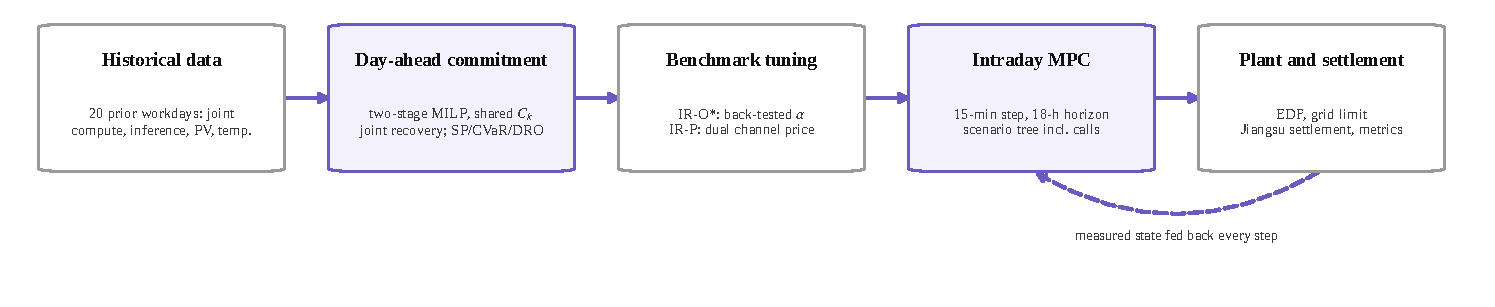
\includegraphics[width=0.98\textwidth]{fig00_framework.pdf}
\caption{Framework of the day-ahead coupled commitment and intraday joint-recovery method. The benchmarks are tuned on
the same historical data before the operating day; the measured state is fed back at every 15-min step.}
\label{fig:framework}
\end{figure*}

\subsection{Day-ahead coupled commitment and its distributionally robust reformulation}
\label{sec:dayahead}

The first-stage decision is the commitment vector $x=(C_k)_{k\in\Kset}$, shared by all scenarios; the second stage is
the joint recovery model of \secref{sec:system}--\ref{sec:model} with one set of operating variables per scenario. The
product $C_kz_{k,\omega}$ in \eqref{eq:valid} is linearised exactly by McCormick inequalities because $z_{k,\omega}$ is
binary. The base model uses five equally likely historical joint scenarios of computing load, inference, PV and
temperature, selected deterministically by load and irradiance quantiles; joint historical days preserve the
coincidence of these drivers. To hedge against an inaccurate empirical distribution, the expected cost is replaced by
its worst case over the $\ell_1$ ball (total-variation ball) around the empirical probabilities $\hat p$,
\begin{gather}
\mathcal P_\delta=\Big\{p\in\mathbb R^{|\Omega|}_{\ge0}:\ \sum_\omega p_\omega=1,\ \sum_\omega|p_\omega-\hat p_\omega|\le\delta\Big\},\nonumber\\
\min_x\ c_0(x)+\max_{p\in\mathcal P_\delta}\sum_\omega p_\omega f_\omega(x),
\label{eq:dro}
\end{gather}
where $f_\omega(x)=\min\{c_\omega^\top y_\omega:\ y_\omega\in\mathcal Y_\omega(x)\}$ is the second-stage cost of scenario
$\omega$, including the binary validity variables of the Jiangsu settlement, and $c_0(x)=-\epsilon\sum_kC_k$ is a tiny
tie-breaking value of committed capacity.

\begin{proposition}[Exact MILP reformulation of the distributionally robust commitment]\label{prop:dro}
For every $\delta\ge0$, problem \eqref{eq:dro} is equivalent to the single-level MILP
\begin{equation}
\begin{aligned}
\min_{x,\,y_\omega,\,\eta,\,\lambda,\,\nu}\ & c_0(x)+\eta+\sum_\omega\hat p_\omega\lambda_\omega+\delta\nu\\
\text{s.t.}\ & c_\omega^\top y_\omega\le\eta+\lambda_\omega,\quad -\nu\le\lambda_\omega\le\nu\qquad\forall\omega\in\Omega,\\
& y_\omega\in\mathcal Y_\omega(x)\quad\forall\omega\in\Omega,\qquad \nu\ge0.
\end{aligned}
\label{eq:droR}
\end{equation}
Moreover, $\delta=0$ yields the two-stage stochastic programme (SP) and $\delta\ge2(1-\min_\omega\hat p_\omega)$ the
scenario-robust problem (RO); for fixed $x$ the worst-case distribution moves the probability mass
$\min\{\delta/2,\,1-\hat p_{\bar\omega}\}$ from the cheapest scenarios to the most expensive scenario $\bar\omega$; and the
optimal value $V(\delta)$ is non-decreasing and concave in $\delta$, with $\nu^*$ a supergradient, \ie\ the marginal
price of robustness.
\end{proposition}

Problem \eqref{eq:droR} adds only $2|\Omega|+1$ continuous variables and $3|\Omega|$ constraints and keeps the binaries
of the second stage, so no semidefinite reformulation or column-and-constraint generation~\cite{zhang2026bilevel,zeng2013}
is needed, which would not be exact with binary recourse. In the same way, $\mathrm{CVaR}_\beta$ and mean--CVaR
objectives are linearised by the Rockafellar--Uryasev formula~\cite{rockafellar2000}. When an event is uncertain, it
appears only in $\mathrm{round}(p_kS)$ of the $S$ scenarios, spread evenly over the load quantiles. As an alternative
scenario generator, all $20\times14=280$ pairs of historical computing days and weather days are clustered by K-means (farthest-point
initialisation, Lloyd iterations) on standardised 12--24~h hourly profiles of deferrable GPUs, inference GPUs and
renewable output (plus the chiller COP in the seasonal-drift test); the medoid of each cluster becomes a scenario and
the cluster share its, generally non-uniform, probability, around which the $\ell_1$ ball is built.

\subsection{Deliverable capability region of commitment vectors}
\label{sec:region}

A single commitment value per event is the current bidding format, but what the data center can actually offer is a
set of commitment vectors. Let all $K$ events with fixed times be called. A vector $C=(C_1,\dots,C_K)\ge0$ is
deliverable if some operation that meets all deadlines and the connection limit achieves a mean reduction of at least
$C_k$ in every event, \ie\ full delivery without shortfall. Denote by $\Cset$ the set of deliverable vectors under
joint recovery (the capability region), by $\Cset_\Pi$ the set under a sequential strategy $\Pi$ (IR-O, IR-O*, IR-P),
and by $\Gamma^0_k$ the stand-alone capability of event $k$.

\begin{proposition}[Capability region and virtual-battery description]\label{prop:region}
(i) $\Cset$ is a bounded convex polytope that is downward closed and contained in the single-event box
$\mathcal B=\prod_k[0,\Gamma^0_k]$. (ii) $\Cset_\Pi\subseteq\Cset$ for every sequential strategy $\Pi$. (iii) For every
block $S=\{i,\dots,j\}$ of consecutive events,
\begin{equation}
\sum_{k\in S}D_kC_k\le\bar b_S:=\bar X(e_j)+E_s^{\max}+H_S+g\,D_S+\Delta_S ,
\label{eq:multibound}
\end{equation}
where $\bar X(e_j)$ is the virtual-storage capacity at the end of the block, $E_s^{\max}$ the dischargeable energy of
full storage, $H_S$ the channel energy of the gaps in the block, $gD_S$ the gas-engine headroom during the events, and
$\Delta_S=\sum_{t\in\Tset_S}(\Pb_t-P^{\mathrm{nom}}_t)\dt$ the difference between the baseline and the same-day import
without response; no unbiased-baseline assumption is needed. Hence $\Cset\subseteq\mathcal V:=\mathcal B\cap\{\sum_{k\in
S}D_kC_k\le\bar b_S\}$, a virtual battery with event power limits $\Gamma^0_k$ that is recharged in the gaps at the
channel width. (iv) Let $h_S=\max\{\sum_{k\in S}D_kC_k:C\in\Cset\}$ and $\mathcal T=\mathcal B\cap\{\sum_{k\in S}D_kC_k\le
h_S,\ |S|\ge2\}$. Then $\theta^*\mathcal T\subseteq\Cset\subseteq\mathcal T$ with $\theta^*=\min_v\min\{1,\theta_v\}$,
$\theta_v=\max\{\theta:\theta v\in\Cset\}$ over the vertices $v$ of $\mathcal T$; $\theta^*=1$ certifies
$\Cset=\mathcal T$. (v) For price coordination, $\Cset_{\mathrm{IR\text{-}P}}\subseteq\Cset_{\mathrm{IR\text{-}P+}}\subseteq\Cset$,
where IR-P+ denotes delivery with the most favourable optimal IT response to the channel price, which a single
combined LP decides.
\end{proposition}

Part (iv) gives a verifiable inner approximation with one LP per support value and per vertex. If $\mathcal V$ or
$\mathcal T$ describes $\Cset$, the data center can bid the event power limits $\Gamma^0_k$ and a few cross-event energy
budgets ($K+1$ numbers in the case study) and the grid operator may call any combination within them. Part (v) reveals
that the response of the IT side to a given channel price is not unique, so a price alone does not determine a
deliverable plan; this motivates the plan--price exchange of \secref{sec:admm}.

\subsection{Intraday rolling joint recovery}
\label{sec:mpc}

On day D, the MPC is re-solved every 15~min over an 18-h horizon (72 steps). The deterministic MPC (JR-D) uses the
historical mean forecast corrected by the error of the last hour; the scenario MPC (JR-S) uses five scenarios with a
non-anticipative first step~\cite{schildbach2014}. Before an uncertain event is confirmed, JR-S represents it by a
scenario tree (the event occurs in three of the five scenarios), whereas the deterministic strategies use the certainty
equivalent (an event with probability of at least 0.5 is treated as called); after confirmation all strategies use the
true state. The terminal storage references come from the day-ahead plan, the settlement of events that are under way
uses the reduction already accrued, and the planner falls back to the rule-based strategy if a solve fails. Within each class, the executed GPUs are assigned to jobs by EDF, which by Lemma~\ref{lem:edf} meets every
deadline.

\subsection{Distributed implementation by plan--price exchange}
\label{sec:admm}

Joint recovery does not require merging the IT scheduler and the facility controller. With the binaries fixed (every
called event valid), the joint model is an LP whose variables split into the IT side $x_{\mathrm{IT}}$ (job execution,
backlog, capping, overheads; cost $f_{\mathrm{IT}}$: delay, overdue and terminal backlog value) and the facility side
$x_{\mathrm F}$ (grid, PV, gas engine, chillers, BESS, TES, settlement; cost $f_{\mathrm F}$). They are coupled only by
the deferrable dynamic IT power $p_t=\pdyn\sum_c(y_{c,t}-\zeta_{c,t})$, one number per step, which appears in
\eqref{eq:cool} and \eqref{eq:elec}; let $q_t$ be the facility's copy. With a price vector $\lambda$ and a penalty
$\rho>0$, the two sides iterate (ADMM~\cite{boyd2011})
\begin{equation}
\begin{aligned}
x_{\mathrm{IT}}^{k+1}&=\arg\min\ f_{\mathrm{IT}}+\lambda^{k\top}p+\tfrac{\rho}{2}\|p-q^k\|^2,\\
x_{\mathrm F}^{k+1}&=\arg\min\ f_{\mathrm F}-\lambda^{k\top}q+\tfrac{\rho}{2}\|q-p^{k+1}\|^2,\\
\lambda^{k+1}&=\lambda^k+\rho\big(p^{k+1}-q^{k+1}\big),
\end{aligned}
\label{eq:admm}
\end{equation}
exchanging only the plans $p^{k+1}$, $q^{k+1}$; the price is updated by both sides with the same formula, and neither
side needs the other's model, state or forecast.

\begin{proposition}[Distributed joint recovery]\label{prop:admm}
(i) The joint model is equivalent to $\min_pF_{\mathrm{IT}}(p)+F_{\mathrm F}(p)$, where both value functions are convex
and piecewise linear. (ii) For every $\rho>0$, the residual $p^k-q^k\to0$, the total cost converges to the joint
optimum and $\lambda^k$ converges to an optimal dual $\lambda^*$ of the coupling. (iii) If the electric chiller is
interior at step $t$, $\lambda^*_t=\varphi_t\dt\,\lch_t$ with $\varphi_t=1+a^{\mathrm{aux}}+\theta/\COP_t$, where
$\lch_t$ is the channel price of Proposition~\ref{prop:price}: the iteration discovers the channel price. (iv) The
quadratic terms make each side's response unique and thereby select a mutually compatible pair among the many optimal
responses to a fixed price.
\end{proposition}

Because glpk cannot solve quadratic programmes, the price term is kept exact and only the proximal term is
approximated by tangent cuts centred at the other side's latest plan, with tangent points densest near zero deviation
($\pm$0.005 to $\pm$20~MW); the approximation error is at most $\rho\delta_p^2/8$ for a tangent spacing $\delta_p$,
and both subproblems remain LPs. In closed loop, JR-A performs $K$ iterations (1--10) per MPC step, warm-started from
the previous step's price and facility plan; any remaining mismatch is absorbed by the grid import.

\subsection{Algorithm flow and computational efficiency}
\label{sec:algorithm}

The complete procedure is summarised in \tabref{tab:algorithm}. Each MPC step solves one MILP whose number of binaries
is the number of remaining events times the number of scenarios (at most 3 for JR-D and 15 for JR-S).
\tabref{tab:timing} reports the model size and median solve time with single-threaded GNU Octave 8.4 and glpk on an
idle machine (experiment~14). Even the 10-scenario MPC solves in less than 2~s, far below the 15-min control interval,
and the deterministic MPC simulates a whole day (120 steps) in about 4~s. The size grows linearly with the number of
scenarios. The day-ahead SP solves in at most 4.3~s and the distributionally robust commitment with ten scenarios in
14--25~s, both as single MILPs, whereas the moment-based DRO planning model of~\cite{zhang2026bilevel} needs eight
column-and-constraint generation iterations and about 850~s.

\begin{table}[!t]
\caption{Algorithm 1: day-ahead coupled commitment and intraday joint-recovery MPC.}
\label{tab:algorithm}
\centering
\fontsize{7.1}{8.7}\selectfont
\begin{tabularx}{\columnwidth}{@{}X@{}}
\toprule
\textbf{Input:} historical day pool $\{\xi_\omega\}$; event notices $(s_k,e_k,\pi_k,p_k$, notice times$)$; baseline
$\Pb$; parameters; risk setting (SP, $\mathrm{CVaR}_\beta$ or DRO $\delta$).\\
\textbf{Output:} commitments $C_k$; 15-min set-points; Jiangsu settlement.\\
\midrule
\textit{Day-ahead (D$-$1)}
\algline{1}{Select $S$ joint scenarios by quantiles (or K-means medoids) with probabilities $\hat p_\omega$; an event with
call probability $p_k<1$ appears in $\mathrm{round}(p_kS)$ scenarios.}
\algline{2}{Solve the two-stage MILP: first stage $C_k$, second stage the joint recovery model per scenario,
$C_kz_{k,\omega}$ linearised by McCormick, risk measure by Proposition~\ref{prop:dro}.}
\algline{3}{Declare $C_k$; store the terminal references $E^{\mathrm{ref}}$, $S^{\mathrm{ref}}$; tune the
benchmarks ($\alpha^*$, IR-P price) on the same data.}
\textit{Intraday (day D, every step $t=1,\dots,T$)}
\algline{4}{Measure the state: backlog per class and deadline, $E_t$, $S_t$, reductions and rebound accrued.}
\algline{5}{Correct the forecasts by the last-hour error; update event calls at confirmation times.}
\algline{6}{Build the $\min(72,T-t+1)$-step joint model: JR-D with the certainty-equivalent events, JR-S with $S$
scenarios and a non-anticipative first step; embed the remaining settlement, rebound windows, lag bounds
\eqref{eq:lag} and terminal values \eqref{eq:term}.}
\algline{7}{Solve the MILP (JR-A: $K$ plan--price iterations \eqref{eq:admm}); on failure fall back to IR-R.}
\algline{8}{Apply the first step: GPUs per class (EDF within the class) and storage/IES set-points; the facility keeps
$\Pg_t\le\Pcap$ by storage first.}
\algline{9}{Record and move to $t+1$.}
\textit{Settlement (end of day D)}
\algline{10}{Settle every event by the Jiangsu rules and compute all indicators of \tabref{tab:metrics}.}\\
\bottomrule
\end{tabularx}
\end{table}

\begin{table}[!t]
\caption{Model size and solve time (median, single-threaded Octave 8.4 with glpk; $T$: horizon in 15-min steps,
$S$: scenarios, $K$: events).}
\label{tab:timing}
\centering\footnotesize
\setlength{\tabcolsep}{3.2pt}
\begin{tabular}{@{}lrrrrrrr@{}}
\toprule
Model & $T$ & $S$ & $K$ & Variables & Binaries & Constraints & Time (s)\\
\midrule
Intraday MPC & 24 & 1 & 3 & 520 & 3 & 392 & 0.007\\
Intraday MPC (JR-D) & 72 & 1 & 3 & 1,193 & 3 & 880 & 0.029\\
Intraday MPC & 72 & 5 & 3 & 5,965 & 15 & 4,444 & 0.48\\
Intraday MPC & 72 & 10 & 3 & 11,930 & 30 & 8,899 & 1.91\\
Intraday MPC & 72 & 5 & 2 & 5,940 & 10 & 4,384 & 0.46\\
Intraday MPC & 72 & 5 & 4 & 5,990 & 20 & 4,504 & 0.49\\
Day-ahead SP & 120 & 5 & 2 & -- & -- & -- & 2.25\\
Day-ahead SP & 120 & 5 & 3 & -- & -- & -- & 2.87\\
Day-ahead SP & 120 & 5 & 4 & -- & -- & -- & 4.32\\
Day-ahead DRO & 120 & 10 & 3 & -- & 30 & -- & 14--25\\
\bottomrule
\end{tabular}
\end{table}

\section{Case analysis}
\label{sec:case}

\subsection{Case settings}
\label{sec:settings}

To verify the effectiveness and applicability of the proposed method, a case study is built entirely from public data.
The deferrable training and batch workload follows the Alibaba PAI GPU cluster trace~\cite{weng2022}, online inference
the Azure LLM inference trace of 2024~\cite{stojkovic2025}, and the weather the ERA5 reanalysis~\cite{hersbach2020} for
Wujiang, Suzhou, retrieved from Open-Meteo; the tariff is the Jiangsu summer TOU tariff of 2025 and the DR rules are
those of Jiangsu~\cite{jiangsu2024dr}. The DR day combines PAI day 27, the weather of 5 August 2024 (maximum
38.3~$^\circ$C) and the Azure trace of 14 May 2024, and the baseline is the mean of the five previous workdays.
\figref{fig:case} shows the inputs: the evening events fall into the TOU peak period after PV output has vanished, and
the grid import without response lies above the baseline during the evening peak because, in normal operation, the
BESS discharges in the peak-price hours that form the baseline.

\begin{figure*}[!t]
\centering
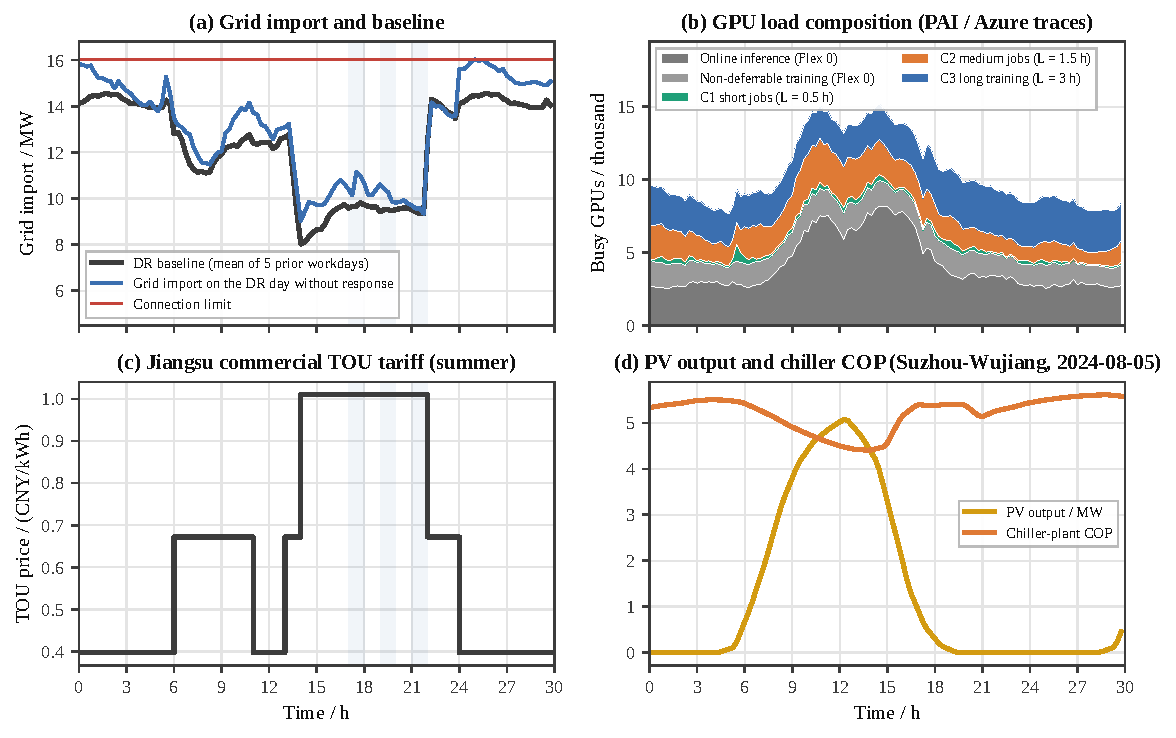
\includegraphics[width=0.86\textwidth]{fig01_case_profiles.pdf}
\caption{Inputs of the case day. (a) DR baseline (mean of the five previous workdays), grid import without response
and connection limit; (b) GPU load composition from the PAI and Azure traces; (c) Jiangsu commercial TOU tariff
(summer); (d) PV output and chiller-plant COP (Wujiang, Suzhou, 5 August 2024). Shaded: the three DR events.}
\label{fig:case}
\end{figure*}

To test the model on LLM-era workloads, the Acme trace of LLM development at the Shanghai AI Laboratory (Seren and
Kalos clusters, March--August 2023)~\cite{hu2024acme} is processed in the same way. It differs strongly from PAI: long
jobs account for 80.5\% of the deferrable GPU$\cdot$h instead of 49.5\%, the GPU$\cdot$h-weighted gang size of the long
class is 407 instead of 35 GPUs, and the load has almost no diurnal cycle (\tabref{tab:acme}). For
\secref{sec:ext-wind}, offshore wind is generated for the Rudong site from ERA5 100-m wind speeds of summer 2024, with a
summer capacity factor of 0.35 and 0.40--0.43 in 17:00--22:00.

Out-of-sample performance is evaluated on 52 operating days: each of the 26 PAI workdays after the DR day is paired with
two different combinations of hot-day weather of summer 2024 and an Azure workday inference trace (a crossed design that
uses no random numbers). The commitments, baseline, scenarios, tuned split $\alpha^*$ and IR-P price are fixed before
the operating day. Statistics are reported as means with 95\% $t$ confidence intervals, and strategies are compared by
paired daily differences with Wilcoxon signed-rank tests. The main parameters are listed in \tabref{tab:params}, with
sources and the parameters of the optional features in \appref{app:data}. Every parameter marked as an assumption is
varied in the sensitivity studies. \tabref{tab:experiments} maps all 26 experiments to the questions they answer.

\begin{table}[!t]
\caption{Main parameters of the case study (sources in \appref{app:data}).}
\label{tab:params}
\centering\footnotesize
\begin{tabularx}{\columnwidth}{@{}>{\raggedright\arraybackslash}p{0.38\columnwidth}X@{}}
\toprule
Parameter & Value\\
\midrule
\multicolumn{2}{@{}l}{\textit{Equipment}}\\
GPUs / node power / idle share & 16,000 / 8.4~kW per 8 GPUs~\cite{latif2024} / 25\%\\
Chiller COP & $6-0.12(T-25)$ in $[3,7]$; 4.41--5.61 on the DR day\\
BESS & 6~MW / 12~MWh, SOC 10--95\%, $\eta=0.95/0.95$, 60~CNY/MWh~\cite{xu2018}\\
TES & 10~MWh$_{\mathrm{th}}$, 4~MW$_{\mathrm{th}}$, $\eta=0.98$, 0.5\%/h\\
Gas engine + absorption & 3~MW, $\eta_{\mathrm e}=0.38$, $\eta_{\mathrm h}=0.45$, 1.5~MW/15~min; COP 0.75\\
PV & 8~MWp, PVWatts v5~\cite{dobos2014}\\
Connection limit $\Pcap=\gamma\hat P$ & $\gamma=1.10\Rightarrow16.03$~MW (1.0--1.3); $P^{\min}=1.5$~MW\\
\multicolumn{2}{@{}l}{\textit{Computing}}\\
Workload & Inference $\approx$25\%, training/batch $\approx$40\% of GPUs, 75\% of it deferrable\\
Lag bounds $L_{1,2,3}$ & 0.5 / 1.5 / 3~h\\
Delay cost / overdue penalty & 0.5 / 1000~CNY per GPU$\cdot$h and hour\\
\multicolumn{2}{@{}l}{\textit{Market and policy}}\\
TOU tariff & Peak 14--22~h ($\times$1.8), valley 0--6~h and 11--13~h ($\times$0.35)\\
DR payment & 3 (E1, E2), 4.2 (E3), 4.8~CNY/kWh (E3 uncertain)\\
Validity / payment cap & $\ge$80\% (+0.1~MW margin) / $\le$120\%\\
Shortfall coefficient $\kappa$ & 1.0 (0.5--2)\\
Rebound charge $\crb$ & 0 and 3~CNY/kW per event (0--6)\\
Gas price & 3.6~CNY/Nm$^3$ (9.89~kWh/Nm$^3$)\\
Emission factors & 0.5617~tCO$_2$/MWh grid~\cite{mee2024ef}; 56.1~t/TJ gas\\
\bottomrule
\end{tabularx}
\end{table}

\begin{table*}[!t]
\caption{Experiments of the case study and where they are reported.}
\label{tab:experiments}
\centering\footnotesize
\setlength{\tabcolsep}{4.5pt}
\begin{tabularx}{\textwidth}{@{}c>{\raggedright\arraybackslash}p{0.21\textwidth}X>{\raggedright\arraybackslash}p{0.14\textwidth}@{}}
\toprule
No. & Experiment & Setting & Reported in\\
\midrule
1 & Cross-event mechanism & Two events; gap $\tau$ 0.25--4~h $\times$ margin $\gamma$ 1.0--1.3; capability ratio & \S\ref{sec:res-mech}, \figref{fig:mech}\\
2 & Case-day closed loop & 8 strategies; coupled and uniform 6-MW commitments; both settlement bases & \S\ref{sec:res-caseday}, \figref{fig:typical}--\ref{fig:flows}\\
3 & Sensitivity (perfect information) & Duration, gap, $\gamma$, commitment; $\tau\times\gamma$ map; hindsight-tuned benchmarks & \S\ref{sec:sens-commit}, \figref{fig:sens}--\ref{fig:map}\\
4 & Out-of-sample evaluation & 52 days; events certain with $\crb=3$ and $\crb=0$; E3 uncertain & \S\ref{sec:res-mc}, \figref{fig:ridge}\\
5 & Channel shadow prices & Duals of the joint plan; KKT residuals & \S\ref{sec:res-price}, \figref{fig:shadow}\\
6 & Commitment--operation pairing & Single-event, scaled single-event and coupled commitments $\times$ IR-O*, JR-D & \S\ref{sec:res-pairing}, \figref{fig:pairing}\\
7 & Ablation and mechanism contribution & No computing flexibility / BESS / TES; waterfall of mechanisms & \S\ref{sec:res-sources}, \figref{fig:decomp}\\
8 & Rebound charge & $\crb$ = 0--6~CNY/kW & \S\ref{sec:sens-rebound}, \figref{fig:rebound}\\
9 & DR payment and shortfall & 1--3~CNY/kWh $\times$ $\kappa$ = 0.5--2 & \S\ref{sec:sens-rebound}, \figref{fig:robust}\\
10 & Realism & Liquid cooling, IT ramp limits, pre-event charge, GPU power capping & \S\ref{sec:sens-real}, \figref{fig:robust}\\
11 & Closed form of Theorem~\ref{thm:closed} & 68 stylised cases, closed form vs LP & \appref{app:proofs}, \figref{fig:theorem}\\
12 & Reliable capacity in closed loop & Uniform 4--9~MW, 20 days & \S\ref{sec:res-capacity}, \figref{fig:capacity}\\
13 & Virtual--physical substitution & BESS 3--24~MWh; $\gamma$ 1.0--1.3; uniform 5--9.5~MW & \S\ref{sec:res-capacity}, \figref{fig:subst}\\
14 & Computational efficiency & Horizon $\times$ scenarios $\times$ events & \S\ref{sec:algorithm}, \tabref{tab:timing}\\
15 & Risk-averse commitment & SP, DRO ($\delta$ = 0.1--1.2), RO, CVaR; 52 days & \S\ref{sec:res-risk}, \figref{fig:risk}\\
16 & Tariff shapes & Five TOU shapes with equal daily mean & \S\ref{sec:sens-gen}, \figref{fig:gen}\\
17 & Multi-energy coupling and policy & Thermal inertia, green share, PUE cap, tie-line ramp & \S\ref{sec:sens-real}, \figref{fig:policy}\\
18 & Season and climate & Suzhou winter, Gui'an summer & \S\ref{sec:sens-gen}, \figref{fig:gen}\\
19 & Job-level validation & PAI/Acme load $\times$ fluid/rigid recovery; 52 days & \S\ref{sec:res-job}, \figref{fig:jobsim}\\
20 & Job mix and overheads & Job sources, gang size $\times$2/$\times$4, checkpoint/restart overheads & \S\ref{sec:res-job}, \figref{fig:jobmix}\\
21 & Green-power direct supply & Offshore wind 0--40~MW behind the meter & \S\ref{sec:ext-wind}, \figref{fig:wind}\\
22 & Pause overhead and capping levels & 6/25-min overheads; one/three capping levels; 26 days & \S\ref{sec:ext-overhead}, \figref{fig:ext}\\
23 & Scenario generation and drift & Quantile vs K-means (+DRO) scenarios; winter day with summer scenarios & \S\ref{sec:res-scen}, \figref{fig:ext}\\
24 & Winter waste-heat recovery & Boiler; heat pump without/with 20 and 40~MWh tanks; 26 winter days & \S\ref{sec:ext-heat}, \figref{fig:heat}\\
25 & Capability region & 91 rays $\times$ 5 strategies; slices; gap $\times$ margin; 52 days & \S\ref{sec:res-region}, \figref{fig:region}\\
26 & Distributed coordination & Plan--price iteration in open loop; JR-A with 1/3/10 exchanges per step; 52 days & \S\ref{sec:res-admm}, \figref{fig:admm}\\
\bottomrule
\end{tabularx}
\end{table*}

\subsection{Cross-event mechanism and closed-loop performance}
\label{sec:res-performance}

\subsubsection{Cross-event recovery mechanism and theoretical checks}
\label{sec:res-mech}

Two events are considered first: a preceding event A from 17:00 and a subsequent event B that starts after a gap
$\tau$. \figref{fig:mech} compares the maximum sustainable reduction $\Gamma_B$ of event B with its stand-alone
capability $\Gamma_B^0$, and \tabref{tab:mech} lists the case with A = 6~MW $\times$ 2~h, B = 1~h and $\gamma=1.10$.
When event A ends, the backlog energy is 4.9~MWh, the storage deficit 12.3~MWh and $\Gamma_B^0\approx8.0$~MW.

\begin{figure*}[!t]
\centering
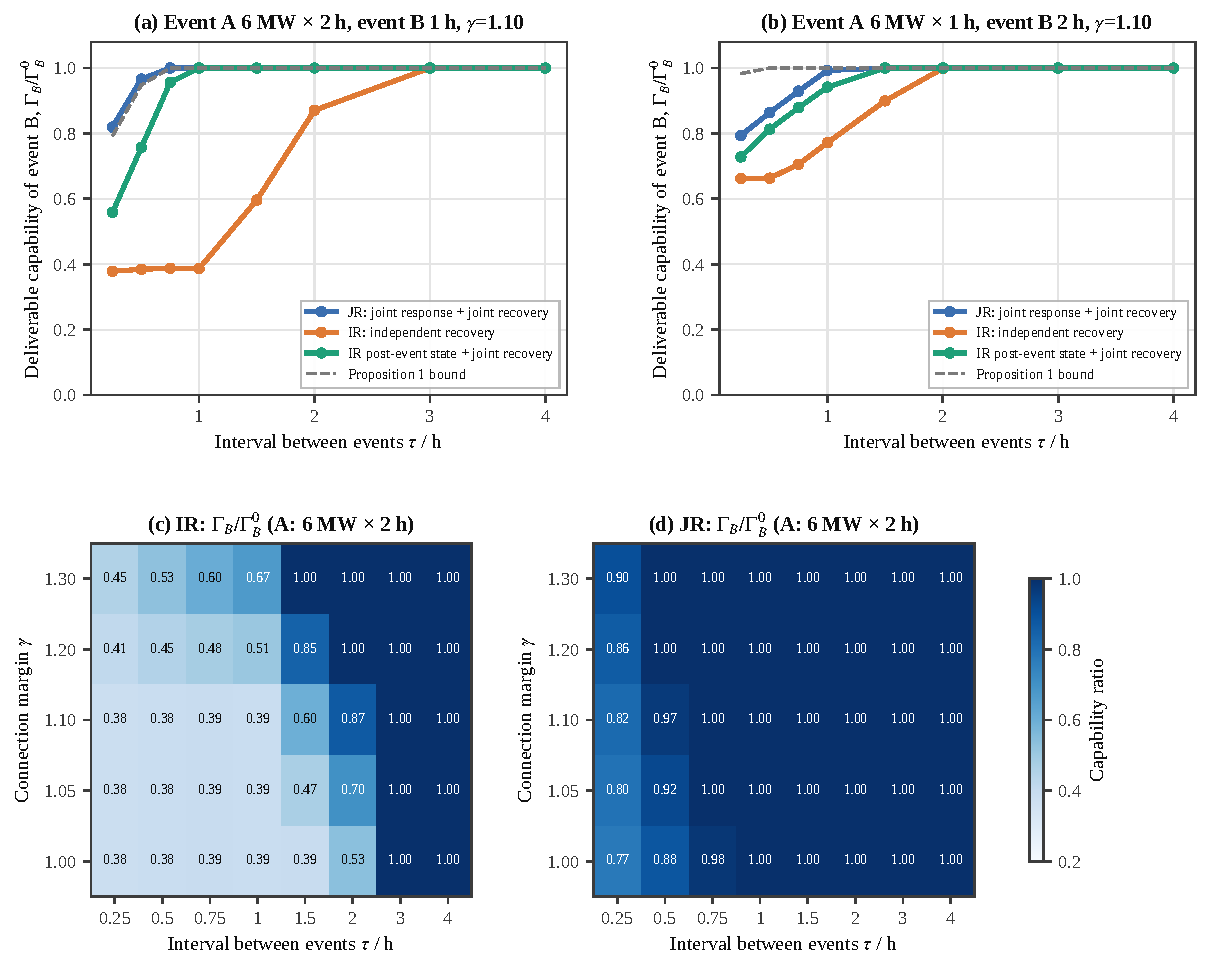
\includegraphics[width=0.84\textwidth]{fig02_mechanism.pdf}
\caption{Cross-event recovery mechanism. (a)(b) Deliverable capability of event B relative to its stand-alone capability
versus the gap ($\gamma=1.10$); (c)(d) capability ratio of independent and joint recovery on the gap--margin plane
(event A: 6~MW $\times$ 2~h).}
\label{fig:mech}
\end{figure*}

\begin{table}[!t]
\caption{Deliverable capability ratio $\Gamma_B/\Gamma_B^0$ (event A 6~MW $\times$ 2~h, event B 1~h, $\gamma=1.10$).}
\label{tab:mech}
\centering\footnotesize
\setlength{\tabcolsep}{3.3pt}
\begin{tabular}{@{}cccccc@{}}
\toprule
Gap $\tau$ (h) & $H$ (MWh) & IR & \makecell{IR state +\\joint recovery} & \makecell{JR (joint response\\and recovery)} & \makecell{Bound of\\Prop.~\ref{prop:bound}}\\
\midrule
0.25 & 1.65 & 0.38 & 0.56 & 0.82 & 0.79\\
0.50 & 3.28 & 0.38 & 0.76 & 0.97 & 0.95\\
0.75 & 4.91 & 0.39 & 0.96 & 1.00 & 1.00\\
1.00 & 6.55 & 0.39 & 1.00 & 1.00 & 1.00\\
1.50 & 9.80 & 0.60 & 1.00 & 1.00 & 1.00\\
2.00 & 13.02 & 0.87 & 1.00 & 1.00 & 1.00\\
\bottomrule
\multicolumn{6}{@{}p{0.97\columnwidth}@{}}{\scriptsize The bound is evaluated at the post-event state of IR, so JR, which also changes the response in event A, may exceed it.}
\end{tabular}
\end{table}

Independent recovery must repay the whole debt before it can respond again: for gaps of up to 1~h, event B retains
only 38--39\% of its stand-alone capability, and 87\% is reached only after 2~h. Joint recovery repays only what the
next event needs. From the same post-event state, a gap of 0.75~h, whose channel energy is only 29\% of the total debt,
already restores 96\%; if the preceding response is planned jointly as well, 0.5~h suffices for 97\%. When event B is
longer (A 1~h, B 2~h), the energy-type limit becomes more prominent: for $\tau\le1$~h, IR reaches 0.66--0.77, joint
recovery from the IR state 0.73--0.94 and JR 0.79--0.99.

The bound of Proposition~\ref{prop:bound} holds in all 80 cases, never exceeding the optimal value from the same
post-event state, and is within 0.05~MW of it in 47 cases; the looser cases occur for $\tau\le0.5$~h, where the
channel width, charging power and EDF order cannot be shifted freely in time while $H$ counts only the total. The
closed form of Theorem~\ref{thm:closed} agrees with the discrete-time LP in all 68 stylised cases to within
$1\times10^{-5}$~MW (\figref{fig:theorem}). With $p_f=5$~MW, $X=5$~MWh and $h=3$~MW, the minimum full-recovery gaps of
IR and JR differ by 0, 0.83, 1.67 and 1.67~h for $L$ = 1, 1.5, 2 and 3~h, exactly $\min(X,p_f(L-D_B))/h$, and joint
recovery has no value when $L=1$~h equals the duration of event B, as predicted by Corollary~\ref{cor:novalue}(a).

\subsubsection{Case-day comparison under identical commitments}
\label{sec:res-caseday}

All strategies are run in closed loop with 15-min steps, the same commitments, SLA and physical constraints, and are
settled by the Jiangsu rules (\tabref{tab:caseday}). Two commitments are used. The coupled day-ahead commitment is
3.27/6.65/7.90~MW for $\crb=3$: because E3 is paid best, the day-ahead model deliberately commits less in E1 and keeps
the channel for E3. For $\crb=0$ it is 8.18/7.98/7.90~MW, equal to the single-event capability assessment. The second
commitment is a uniform 6~MW per event.

\begin{table*}[!t]
\caption{Case-day results: fulfilment / valid events / maximum rebound (MW) / total cost ($10^4$~CNY).}
\label{tab:caseday}
\centering\footnotesize
\setlength{\tabcolsep}{4.2pt}
\begin{tabular}{@{}llllllc@{}}
\toprule
Commitment and settlement & IR-O* & IR-P & JR-M & \textbf{JR-D} & JR-S & JR-oracle\\
\midrule
Coupled, $\crb=3$ & 100\% / 3 / 6.39 / 24.35 & 100\% / 3 / 4.16 / 23.31 & 86.0\% / 2 / 6.44 / 28.01 & \textbf{99.9\% / 3 / 5.02 / 22.71} & 100\% / 3 / 3.48 / 22.76 & 22.66\\
Uniform 6~MW, $\crb=3$ & 100\% / 3 / 6.45 / 24.57 & 96.6\% / 3 / 4.37 / 23.61 & 92.4\% / 2 / 6.44 / 26.42 & \textbf{100\% / 3 / 5.77 / 22.84} & 100\% / 3 / 4.77 / 22.85 & 22.80\\
Coupled, $\crb=0$ & 80.3\% / 2 / -- / 22.70 & 73.7\% / 1 / -- / 24.70 & 84.4\% / 2 / -- / 24.60 & \textbf{99.3\% / 3 / -- / 19.13} & 99.6\% / 3 / -- / 19.12 & 19.04\\
Uniform 6~MW, $\crb=0$ & 100\% / 3 / -- / 19.97 & 92.6\% / 3 / -- / 20.42 & 99.8\% / 3 / -- / 20.81 & \textbf{100\% / 3 / -- / 19.34} & 100\% / 3 / -- / 19.36 & --\\
\bottomrule
\multicolumn{7}{@{}l@{}}{\scriptsize With $\crb=0$ all strategies raise the import to near the connection limit after the events (maximum rebound 6.52~MW), so the rebound is not listed.}
\end{tabular}
\end{table*}

\begin{figure*}[!t]
\centering
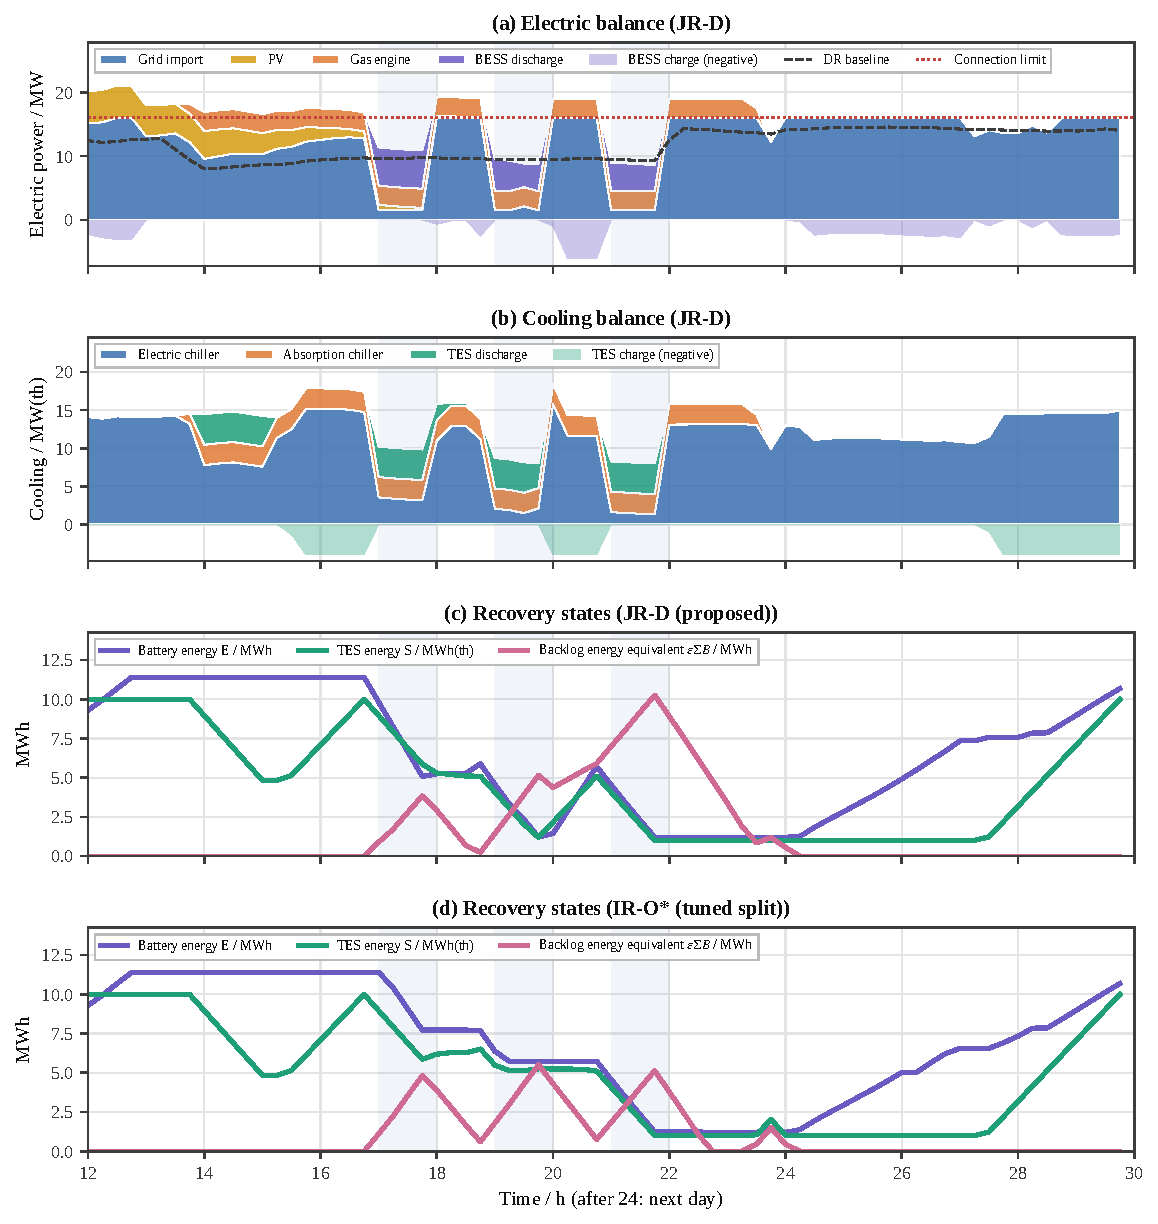
\includegraphics[width=0.80\textwidth]{fig18_typical_day.pdf}
\caption{Operation on the case day (rule setting, coupled commitment 8.18/7.98/7.90~MW). (a) Electricity balance and
(b) cooling balance of JR-D; (c)(d) recovery states of JR-D and IR-O*: BESS energy, TES energy and the electricity
equivalent of the backlog $\varepsilon\sum_cB_c$.}
\label{fig:typical}
\end{figure*}

\begin{figure*}[!t]
\centering
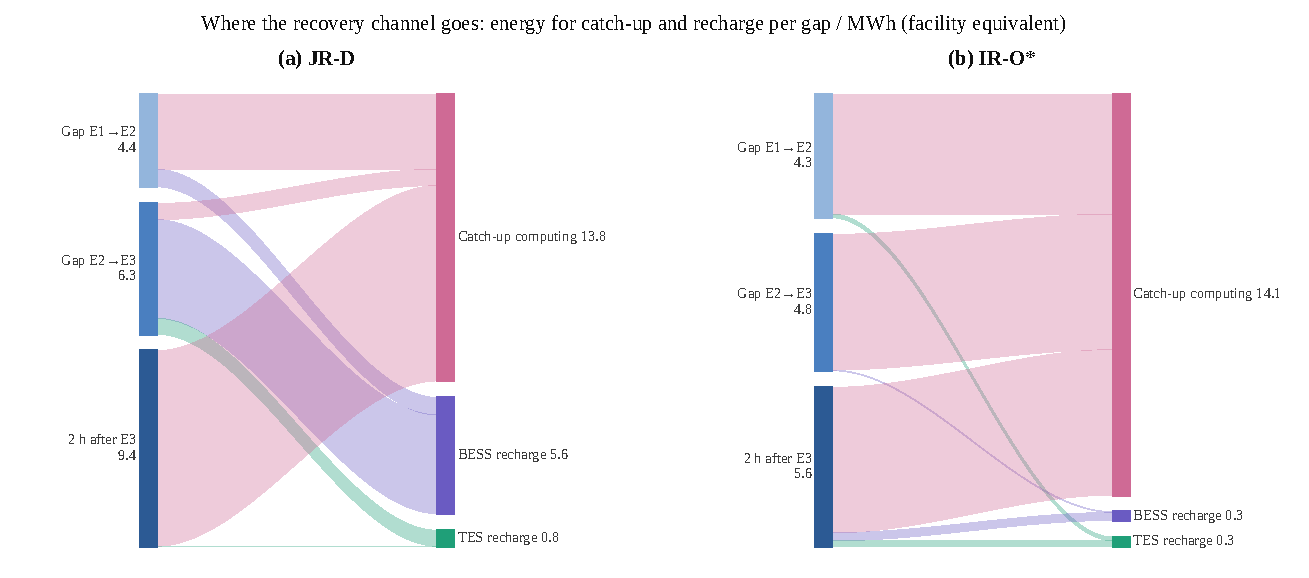
\includegraphics[width=0.78\textwidth]{fig19_channel_flows.pdf}
\caption{Use of the recovery channel in each gap and in the 2~h after E3 (same setting as \figref{fig:typical}):
energy for catch-up computing, BESS recharging and TES recharging.}
\label{fig:flows}
\end{figure*}

Joint recovery is most valuable when the commitments approach the single-event capabilities. In the rule setting with
the coupled commitment, JR-D keeps all three events valid (fulfilment 99.3\%), whereas the strongest independent
benchmark IR-O* fulfils 80.3\% and loses E2; the total cost of JR-D is 15.7\% lower than that of IR-O* and 22.5\% lower
than that of IR-P. \figref{fig:typical} and \figref{fig:flows} show why. JR-D defers more long-lag work during E2, so
that a backlog of 6,027~GPU$\cdot$h, about 10~MWh of facility electricity, is carried into E3; the channel between E2
and E3 is used mainly to recharge the BESS and TES (5.6 and 0.8~MWh), and the backlog is worked off after E3. IR-O*
spends almost the whole channel of the three gaps on catch-up computing (14.1~MWh) and recharges only 0.3~MWh of
storage; in E2 its energy management gives up validity (delivering 4.76~MW) to save the BESS for the better-paid E3,
and IR-P delivers only 3.40~MW in E2.

With moderate commitments (uniform 6~MW), IR-O* and IR-P keep all three events valid as well, and the advantage of JR-D
shrinks to 3.2\% against IR-O* in the rule setting and 3.3\% against IR-P in the rebound-priced setting. In the rebound-priced setting the
advantage comes mainly from the rebound charge: of the $-2.6\%$ and $-3.3\%$ against IR-P, only $+1.1\%$ and $-0.6\%$
remain when the rebound charge is excluded, because the charge makes the channel expensive after each event and joint
recovery moves catch-up to cheaper hours. Price coordination does not replace joint recovery: IR-P is the strongest
benchmark in the rebound-priced setting but the weakest with high commitments in the rule setting (73.7\%), because a
one-shot day-ahead price is no longer correct once the state deviates from the plan and because the non-unique LP
response lets the IT side crowd the channel again (Proposition~\ref{prop:price}). Cross-event foresight is essential:
the event-by-event JR-M fulfils 84--92\% and costs 8--19\% more than JR-D. The scenario MPC and the perfect-information
reference differ from JR-D by less than 0.5\%.

\subsubsection{Out-of-sample performance on 52 operating days}
\label{sec:res-mc}

\tabref{tab:mc} reports the 52 operating days with a uniform commitment of 6~MW for three settings, and
\figref{fig:ridge} shows the full cost distributions (the box plots are given in \figref{fig:mcbox}). The distribution
of JR-D is shifted to the left as a whole and has the shortest right tail.

\begin{table}[!t]
\caption{Out-of-sample results on 52 operating days (uniform 6~MW; means, 95\% CI in brackets).}
\label{tab:mc}
\centering\footnotesize
\setlength{\tabcolsep}{2.6pt}
\begin{tabular}{@{}lcccc@{}}
\toprule
Strategy & \makecell{Fulfilment\\(\%)} & \makecell{All\\valid} & \makecell{Max rebound\\(MW)} & \makecell{Total cost\\($10^4$~CNY)}\\
\midrule
\multicolumn{5}{@{}l}{\textit{Events certain, $\crb=3$~CNY/kW}}\\
IR-R & 71.1 [66.4, 75.7] & 11.5\% & 6.52 & 30.25 [29.18, 31.33]\\
IR-O & 81.6 [76.9, 86.2] & 48.1\% & 6.28 & 26.00 [24.91, 27.09]\\
IR-O* & 97.8 [96.5, 99.1] & 90.4\% & 6.22 & 24.30 [23.45, 25.15]\\
IR-P & 98.3 [96.7, 99.9] & 94.2\% & 5.30 & 23.20 [22.46, 23.94]\\
JR-M & 91.7 [89.6, 93.8] & 48.1\% & 6.35 & 24.81 [23.78, 25.84]\\
\textbf{JR-D} & \textbf{99.9 [99.7, 100]} & \textbf{100\%} & \textbf{4.85} & \textbf{22.53 [21.79, 23.27]}\\
\multicolumn{5}{@{}l}{\textit{Events certain, $\crb=0$ (Jiangsu settlement only)}}\\
IR-O* & 99.2 [98.5, 99.9] & 98.1\% & 6.5 & 19.71 [19.07, 20.35]\\
IR-P & 93.3 [90.7, 96.0] & 86.5\% & 6.5 & 20.21 [19.42, 20.99]\\
JR-M & 94.6 [92.5, 96.6] & 67.3\% & 6.5 & 21.38 [20.39, 22.36]\\
\textbf{JR-D} & \textbf{99.9 [99.7, 100]} & \textbf{100\%} & 6.5 & \textbf{19.10 [18.54, 19.67]}\\
\multicolumn{5}{@{}l}{\textit{E3 called with probability 0.6, confirmed 1~h ahead, $\crb=3$}}\\
IR-O* & 98.2 & 94.2\% & -- & 24.26\\
IR-P & 97.6 & 94.2\% & -- & 23.67\\
JR-M & 94.9 & 67.3\% & -- & 24.10\\
JR-D & 99.98 & 100\% & -- & 22.74\\
JR-S (scenario tree) & 99.7 & 100\% & -- & 22.65\\
JR-oracle & 100.0 & 100\% & -- & 22.27\\
\bottomrule
\end{tabular}
\end{table}

\begin{figure*}[!t]
\centering
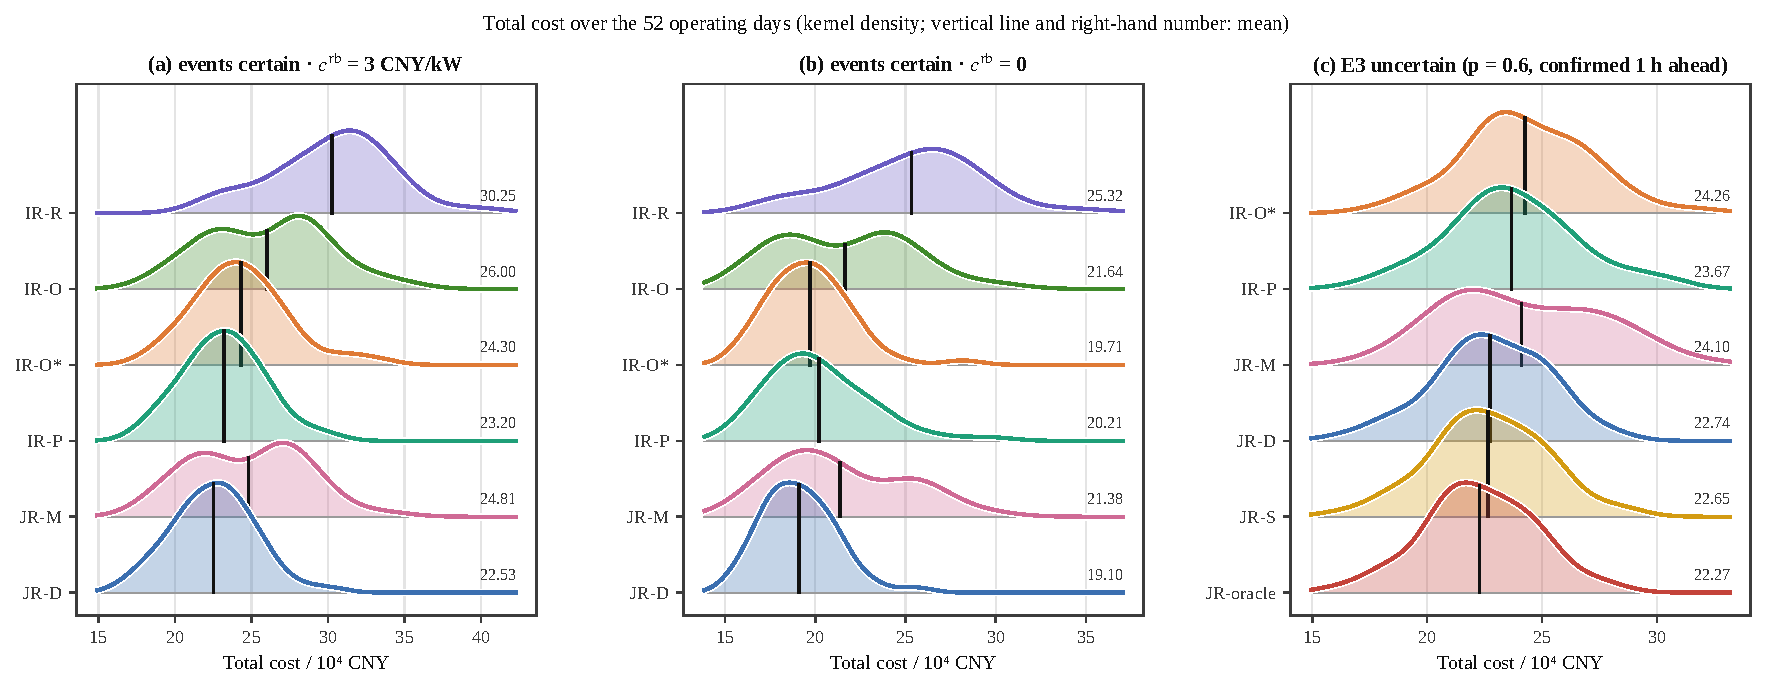
\includegraphics[width=0.94\textwidth]{fig24_ridge_montecarlo.pdf}
\caption{Kernel densities of the daily total cost on the 52 operating days for the three settings (vertical lines and
right-hand numbers: means, $10^4$~CNY).}
\label{fig:ridge}
\end{figure*}

With events certain and the rebound priced, the paired daily difference of JR-D against IR-P is $-6{,}692$~CNY per day
(95\% CI $[-7{,}891,-5{,}492]$, $-2.9\%$, $p=4\times10^{-10}$, cheaper on 50 of the 52 days), with a 8.4\% lower maximum
rebound and 1.6 percentage points higher fulfilment; against IR-O* the cost is 7.3\% lower on all 52 days and the
maximum rebound 22.0\% lower; against JR-M the cost is 9.2\% lower (52/52 days) and the fulfilment 8.2 points higher.
Excluding the rebound charge, the difference to IR-P ($-0.7\%$) is not significant ($p=0.64$), and that to IR-O* is
$+0.9\%$. In the rule setting, JR-D costs 3.1\% less than IR-O* ($-6{,}062$~CNY per day $[-7{,}053,-5{,}072]$, 52/52 days,
$p=4\times10^{-10}$) and 5.5\% less than IR-P; all strategies then raise the import to about 6.5~MW above the baseline
after the events. When E3 is uncertain, JR-D costs 4.0\% less than IR-P (51/52 days) and 6.3\% less than IR-O*. The
scenario MPC gains little: JR-S is 0.4\% cheaper than JR-D ($-821$~CNY per day $[-2{,}064,+421]$, $p=0.46$), saving
5,400~CNY on days when E3 is not called and losing 2,300~CNY on days when it is, so the scenario tree trades part of
the value of called days for a hedge against cancellation. JR-D is 2.1\% above perfect information, mostly because of
the rebound charge (0.2\% without it, $p=0.43$). In summary, against the strongest benchmark of each setting, joint
recovery is 2.9--4.0\% cheaper and keeps all events valid on every day, whereas the benchmarks achieve this on 86--98\%
of the days.

\subsubsection{Sources of benefit and contribution of the mechanisms}
\label{sec:res-sources}

\tabref{tab:ablation} isolates the resources (uniform 6~MW, $\crb=3$, perfect information). Without computing
flexibility ($L=0$) the two strategies are identical: with a single recovery state there is nothing to coordinate. Even
with the hindsight-optimal static split ($\alpha^*=0.9$, fulfilment 100\%), joint recovery is still 6.9\% cheaper.

\begin{table}[!t]
\caption{Ablation (uniform 6~MW, $\crb=3$, perfect information; fulfilment / total cost in $10^4$~CNY).}
\label{tab:ablation}
\centering\footnotesize
\begin{tabular}{@{}lccc@{}}
\toprule
Configuration & IR-O & JR & JR vs IR-O\\
\midrule
Full system & 89.2\% / 25.58 & 100\% / 22.80 & $-10.9\%$\\
No computing flexibility ($L=0$) & 29.0\% / 28.72 & 29.0\% / 28.72 & 0\\
No BESS & 16.4\% / 35.54 & 36.1\% / 32.38 & $-8.9\%$\\
No TES & 68.1\% / 27.03 & 100\% / 23.49 & $-13.1\%$\\
IR-O with hindsight split $\alpha^*=0.9$ & 100\% / 24.49 & -- & $-6.9\%$\\
\bottomrule
\end{tabular}
\end{table}

\begin{figure*}[!t]
\centering
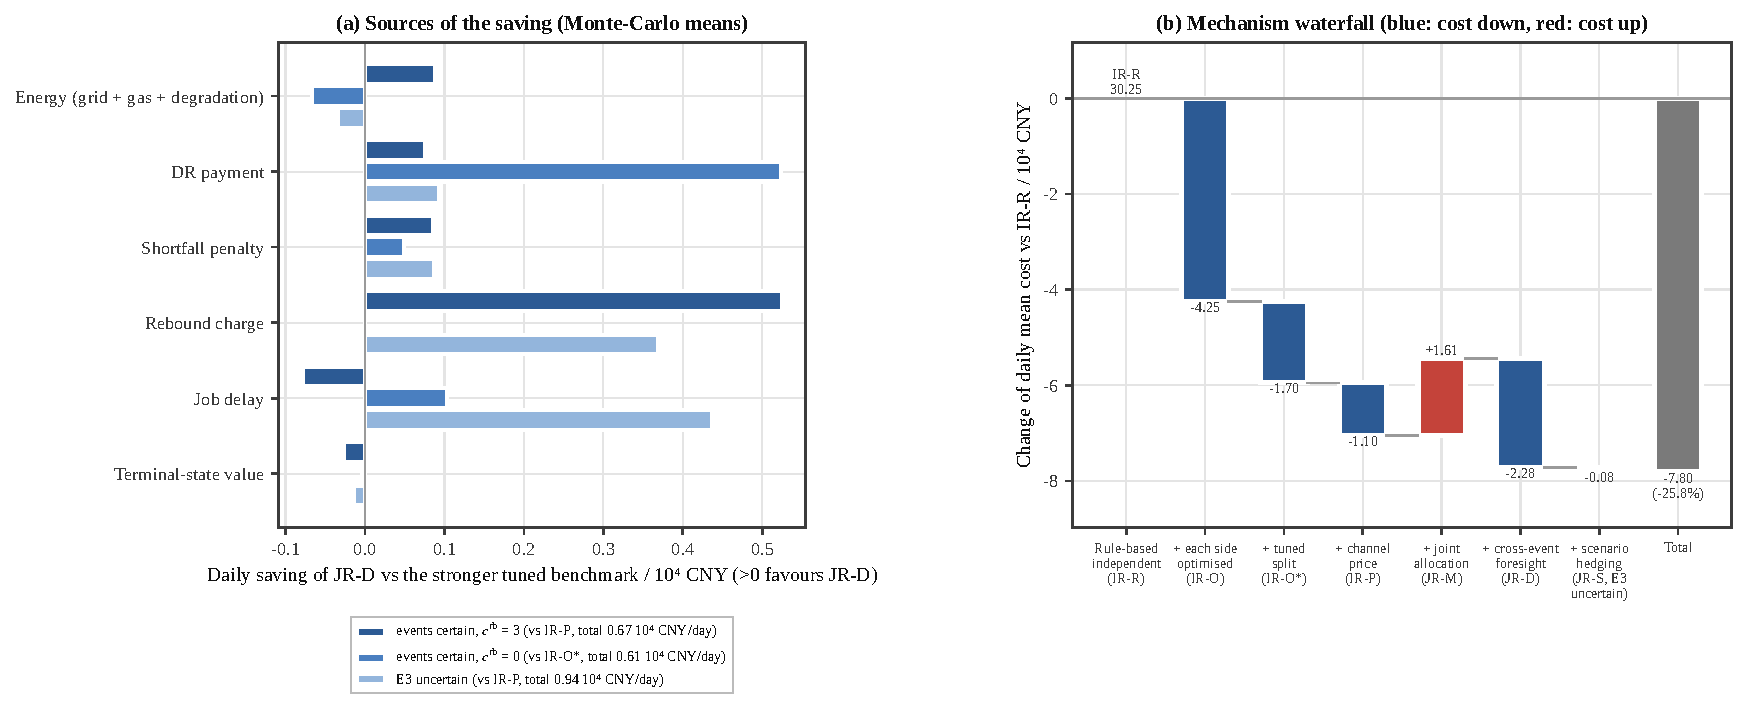
\includegraphics[width=0.94\textwidth]{fig16_decomposition.pdf}
\caption{(a) Daily saving of JR-D against the stronger tuned benchmark, decomposed by source (means over the 52 days);
(b) contribution of each coordination mechanism, starting from rule-based independent recovery (events certain,
$\crb=3$; the last step uses the uncertain-E3 setting).}
\label{fig:decomp}
\end{figure*}

\figref{fig:decomp}(b) adds one coordination mechanism at a time to the rule-based IR-R (30.25$\times10^4$~CNY per day):
optimising each side ($-4.25$), tuning the split on history ($-1.70$), sending the channel price ($-1.10$), allocating
the channel jointly but event by event ($+1.61$), adding cross-event foresight ($-2.28$) and hedging the uncertain event
by scenarios ($-0.08$), a total of $-7.80\times10^4$~CNY ($-25.8\%$). Optimising each side and cross-event foresight
contribute most. Joint allocation without foresight (JR-M) is worse than price coordination, because after each event it
catches up or recharges as if only one more event followed and often spends the channel on the wrong state; joint
allocation and cross-event foresight are both needed.

\figref{fig:decomp}(a) decomposes the daily saving of JR-D against the stronger benchmark. With the rebound priced, 78\%
of the saving of $0.67\times10^4$~CNY against IR-P comes from the rebound charge. In the rule setting, 86\% of the
saving of $0.61\times10^4$~CNY against IR-O* comes from the additional DR payment of keeping all three events valid.
When E3 is uncertain, the largest item is the job-delay cost ($0.44$ of $0.94\times10^4$~CNY), because the IT side of
IR-P follows the day-ahead price and defers too much while the call of E3 is unknown. The energy cost hardly changes in
any setting: joint recovery does not save money by more arbitrage.

\subsection{Deliverable capacity, channel price and coordination}
\label{sec:res-capacity-all}

\subsubsection{Reliably deliverable capacity and virtual--physical substitution}
\label{sec:res-capacity}

In the rule setting, each uniform commitment from 4 to 9~MW was run on 20 operating days in closed loop
(\tabref{tab:capacity}, \figref{fig:capacity}). Requiring all three events to be valid on at least 95\% of the days,
IR-O* can commit 6~MW, IR-P reaches this reliability at no commitment level, and JR-D can commit 8~MW, which is 33\%
more. At the respective best commitments, JR-D (7~MW, $18.89\times10^4$~CNY per day) is 4.1\% cheaper than IR-O* (6~MW,
$19.70\times10^4$~CNY per day).

\begin{table}[!t]
\caption{Closed-loop reliability by uniform commitment (rule setting, 20 days): share of days with all events valid /
mean total cost ($10^4$~CNY).}
\label{tab:capacity}
\centering\footnotesize
\begin{tabular}{@{}cccc@{}}
\toprule
Commitment (MW) & IR-O* & IR-P & \textbf{JR-D}\\
\midrule
4 & 75\% / 21.63 & 85\% / 21.42 & \textbf{100\% / 20.69}\\
5 & 80\% / 20.83 & 75\% / 21.05 & \textbf{100\% / 19.75}\\
6 & 95\% / 19.70 & 80\% / 20.27 & \textbf{100\% / 19.05}\\
7 & 80\% / 20.32 & 70\% / 20.34 & \textbf{95\% / 18.89}\\
8 & 50\% / 21.38 & 40\% / 21.65 & \textbf{95\% / 19.20}\\
9 & 25\% / 22.97 & 25\% / 23.42 & 65\% / 21.01\\
\bottomrule
\end{tabular}
\end{table}

\begin{figure*}[!t]
\centering
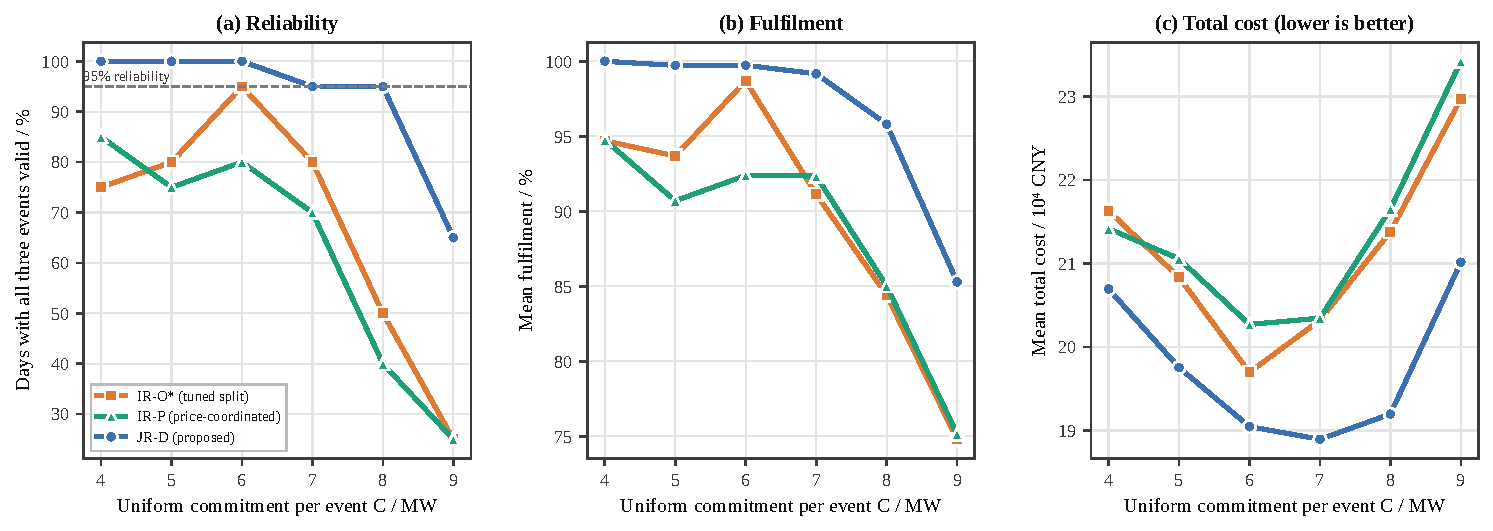
\includegraphics[width=0.94\textwidth]{fig11_capacity.pdf}
\caption{Closed-loop reliability, fulfilment and total cost versus the uniform commitment (rule setting, 20 operating
days).}
\label{fig:capacity}
\end{figure*}

The virtual--physical substitution experiment sweeps the BESS energy (at 6~MW power and a fixed absolute connection
limit) and the connection margin $\gamma$ under perfect information and finds the largest uniform commitment that is
fulfilled at $\ge$99\% with all events valid (\tabref{tab:subst}, \figref{fig:subst}). Joint recovery is worth about
9--12~MWh of battery: JR reaches 6.5~MW with a 3-MWh battery, which IR-O* needs 12~MWh for; JR reaches 7.0~MW with
6~MWh, which IR-O* needs 15--18~MWh for; and JR reaches 8.0~MW with 12~MWh, which independent recovery does not reach
with any battery size. Joint recovery is also worth about 2.9~MW of connection capacity: JR reaches 8.0~MW at
$\gamma=1.10$, whereas IR-O* needs $\gamma=1.30$, \ie\ $0.2\times14.57\approx2.9$~MW more; the 7.0~MW of JR at
$\gamma=1.00$ likewise requires $\gamma=1.20$ for IR-O*. At its reliable capacity, JR carries a long-lag backlog worth
6.0--7.0~MWh into E3, about half of the 12-MWh battery (\figref{fig:subst}(c)); the smaller the battery, the more this
virtual computing storage is used, and with 18~MWh or more the physical storage suffices and joint recovery no longer
needs it.

\begin{table}[!t]
\caption{Reliable uniform commitment (MW, $\ge$99\% fulfilment with all events valid, perfect information).}
\label{tab:subst}
\centering\footnotesize
\setlength{\tabcolsep}{3.6pt}
\begin{tabular}{@{}lccccccc@{}}
\toprule
BESS energy (MWh) & 3 & 6 & 9 & 12 & 15 & 18 & 24\\
\midrule
JR & 6.5 & 7.0 & 7.5 & \textbf{8.0} & 7.5 & 7.0 & 6.5\\
IR-O* (hindsight) & -- & 5.0 & 6.0 & 6.5 & 7.0 & 7.0 & 6.5\\
IR-P & -- & 5.0 & 5.5 & 6.0 & 5.0 & -- & --\\
Backlog carried into E3 by JR (MWh) & 6.8 & 7.0 & 7.0 & 6.0 & 3.5 & 0.8 & 0\\
\midrule
Connection margin $\gamma$ & 1.00 & 1.05 & 1.10 & 1.15 & 1.20 & 1.30 & \\
\midrule
JR & 7.0 & 7.5 & \textbf{8.0} & 8.0 & 8.0 & 8.0 & \\
IR-O* (hindsight) & 6.0 & 6.0 & 6.5 & 6.5 & 7.0 & 8.0 & \\
IR-P & 5.0 & 5.5 & 6.0 & 7.0 & 6.0 & 6.0 & \\
\bottomrule
\multicolumn{8}{@{}l@{}}{\scriptsize --: not reached within the sweep (5--9.5~MW).}
\end{tabular}
\end{table}

\begin{figure*}[!t]
\centering
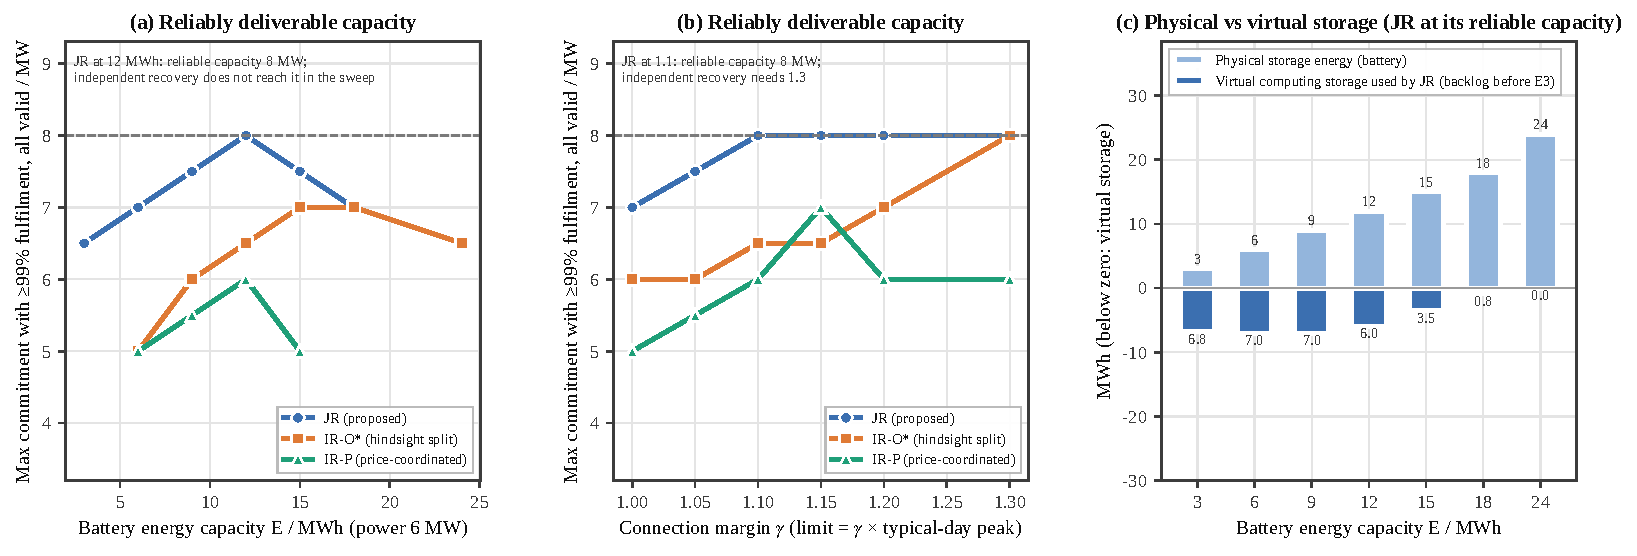
\includegraphics[width=0.96\textwidth]{fig14_substitution.pdf}
\caption{Virtual--physical substitution. (a)(b) Reliably deliverable capacity versus BESS energy and connection margin
(dashed: JR in the base configuration); (c) physical battery energy and the virtual computing storage used by JR
(backlog energy carried into E3) at its reliable capacity.}
\label{fig:subst}
\end{figure*}

Larger batteries are not always better. Beyond 12--15~MWh the reliable capacity of all strategies falls, because in
normal operation a larger battery discharges in the peak-price hours for arbitrage and thereby lowers the
five-day-average baseline: every additional 6~MWh lowers the baseline in the event hours by about 0.6~MW (E1:
10.28~MW with 6~MWh, 8.47~MW with 24~MWh), shrinking the room for reductions measured against it. DR contracts should
therefore consider battery sizing and baseline rules together.

\subsubsection{Shadow prices: scarcity of the recovery channel}
\label{sec:res-price}

With perfect information and a uniform 6~MW, the duals of the joint plan (binaries fixed) reveal the scarcity of the
channel (\tabref{tab:shadow}, \figref{fig:shadow}). Without a rebound charge, the physical connection limit itself
creates competition in the gaps: at $\gamma=1.10$ its shadow price is 1,260--1,455~CNY/MWh (1,771--2,242 at
$\gamma=1.00$), so the channel price is 2.2--3.2 times the peak tariff. With the rebound charge, the binding constraint
becomes the rebound window (3,000~CNY/MWh) and the connection limit is slack. Proposition~\ref{prop:price} is confirmed
numerically: at all interior charging, discharging and catch-up steps of the four settings, the residuals of
$\eta_{\mathrm{c}}\nu_t=\lambda_t+\cdeg$, $\nu_t/\eta_{\mathrm{d}}=\lambda_t-\cdeg$ and $\mu_{c,t}=\varepsilon_t\lambda_t$
are at most $2\times10^{-12}$; for example, $\mu=3.94$~CNY per GPU$\cdot$h in the first gap divided by
$\varepsilon\approx0.99$~kWh per GPU$\cdot$h equals the channel price of about $4.0\times10^3$~CNY/MWh. Long-lag backlog
is the cheapest state: in E3 the marginal cost of C3 backlog (3.19) is well below that of C1 (4.38) because its
deadline lies after E3, so the channel goes first to storage recharging and short-lag catch-up and the long-lag work is
carried across the event, as Theorem~\ref{thm:closed} predicts for several classes.

\begin{table}[!t]
\caption{Shadow prices of the joint plan (CNY/MWh; marginal backlog cost $\mu$ in CNY per GPU$\cdot$h).}
\label{tab:shadow}
\centering\footnotesize
\setlength{\tabcolsep}{3.2pt}
\begin{tabular}{@{}lccccc@{}}
\toprule
Period & $\lambda_t$ & $\lambda^{\mathrm{cap}}_t$ & $\lambda^{\mathrm{rb}}_t$ & $\nu_t$ & $\mu_{1}$ / $\mu_{2}$ / $\mu_{3}$\\
\midrule
\multicolumn{6}{@{}l}{\textit{$\gamma=1.10$, $\crb=3$~CNY/kW}}\\
Gap E1--E2 & 4010 & 0 & 3000 & 4223 & 3.94 / 3.94 / 3.94\\
Gap E2--E3 & 4010 & 0 & 3000 & 4223 & 3.92 / 3.88 / 3.69\\
Event E3 & 4505 & 0 & 0 & 4223 & 4.38 / 3.43 / \textbf{3.19}\\
\multicolumn{6}{@{}l}{\textit{$\gamma=1.10$, $\crb=0$}}\\
Gap E1--E2 & 2464 & \textbf{1455} & 0 & 2657 & 2.49 (all classes)\\
Gap E2--E3 & 2270 & \textbf{1260} & 0 & 2522 & 2.22 (all classes)\\
\multicolumn{6}{@{}l}{\textit{$\gamma=1.00$, $\crb=0$}}\\
Gap E1--E2 & 3252 & \textbf{2242} & 0 & 3285 & 3.16 (all classes)\\
Gap E2--E3 & 2781 & \textbf{1771} & 0 & 3060 & 2.72 (all classes)\\
\bottomrule
\end{tabular}
\end{table}

\begin{figure*}[!t]
\centering
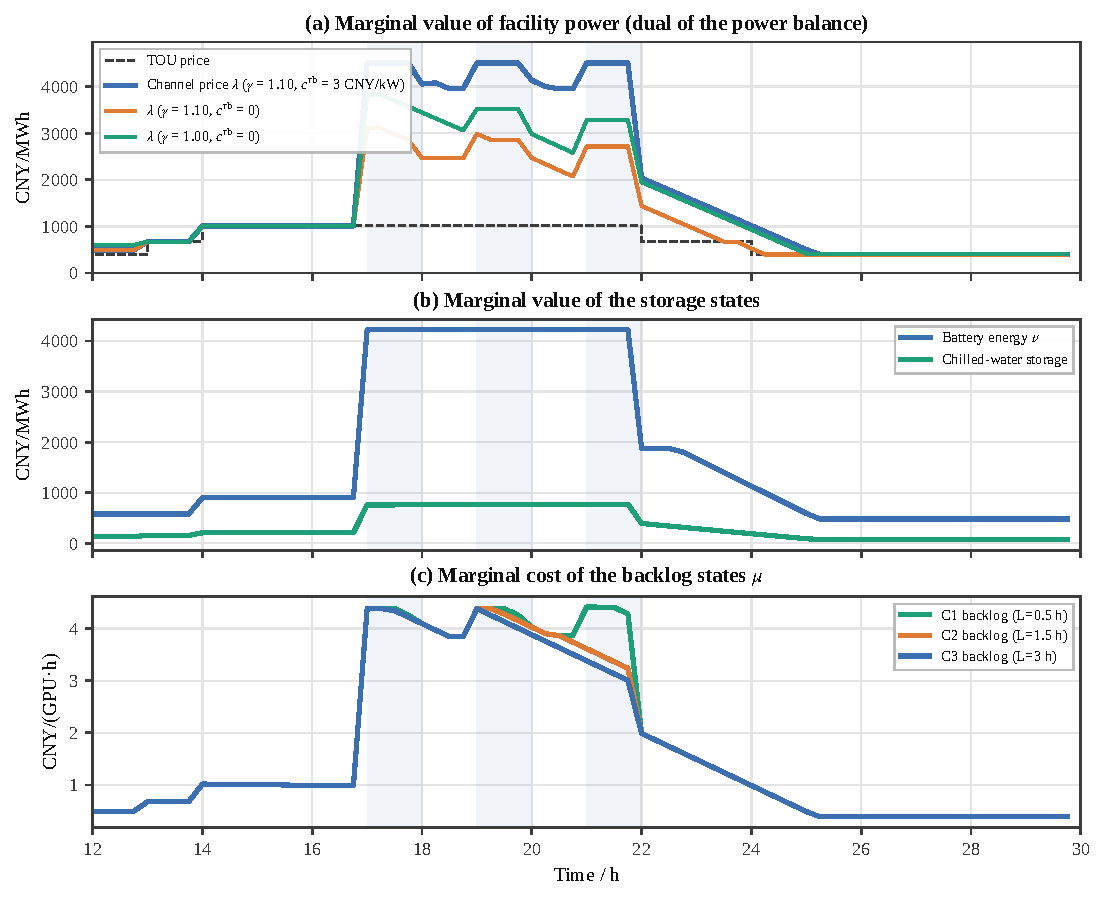
\includegraphics[width=0.80\textwidth]{fig08_shadow_prices.pdf}
\caption{Shadow prices of the joint plan (uniform 6~MW, perfect information). (a) Marginal value of facility electricity
(channel price); (b) marginal value of the storage states; (c) marginal cost of the backlog of each class.}
\label{fig:shadow}
\end{figure*}

\subsubsection{Cross-event capability region}
\label{sec:res-region}

The previous subsections compared strategies for given commitments. When bidding day-ahead, the data center needs to
know which commitment vectors $(C_1,C_2,C_3)$ it can deliver in full. Experiment~25 computes the capability region of
Proposition~\ref{prop:region} under perfect information along 91 rays $C=t\,d$ ($d$ on a simplex grid), together with the
deliverable sets of the benchmarks, the multi-event energy bound and the vertex certificate, for the base case (gap
1~h, $\gamma=1.10$) and a tight case (gap 0.5~h, $\gamma=1.00$). IR-O* uses the hindsight-optimal split for every ray,
the upper limit of any static split (\tabref{tab:region}, \figref{fig:region}).

\begin{table}[!t]
\caption{Capability region of the three events (perfect information).}
\label{tab:region}
\centering\footnotesize
\setlength{\tabcolsep}{1.5pt}
\begin{tabular}{@{}lcc@{}}
\toprule
 & \makecell{Base\\($\tau=1$~h, $\gamma=1.10$)} & \makecell{Tight\\($\tau=0.5$~h, $\gamma=1.00$)}\\
\midrule
Stand-alone capability $\Gamma^0_{1,2,3}$ (MW) & 8.18 / 7.98 / 7.90 & 8.18 / 8.05 / 8.06\\
Support $h_{123}$ of JR (sum of $\Gamma^0_k$) & 24.06 (24.06) & 19.43 (24.29)\\
Energy bound $\bar b$ (MWh) & \makecell{25.66 = 11.36 + 11.41\\ + 9.07 $-$ 6.17} & \makecell{19.57 = 11.58 + 11.40\\ + 2.93 $-$ 6.34}\\
Template $\mathcal T$ & exact (8 vertices) & $\theta^*=0.9997$ (10 vertices)\\
\makecell[l]{Uniform capability (MW):\\JR / IR-P+ / IR-O* / IR-O / IR-P} & \makecell{7.90 / 7.90 / 6.44 /\\ 5.50 / 4.52} & \makecell{6.48 / 6.47 / 6.44 /\\ 3.05 / 2.55}\\
\makecell[l]{Region volume relative to JR:\\IR-P+ / IR-O* / IR-O / IR-P} & \makecell{1.000 / 0.966 /\\ 0.770 / 0.279} & \makecell{0.850 / 0.962 /\\ 0.278 / 0.119}\\
\bottomrule
\multicolumn{3}{@{}p{0.97\columnwidth}@{}}{\scriptsize Energy bound = virtual storage + storage + channel + baseline difference.}
\end{tabular}
\end{table}

\begin{figure*}[!t]
\centering
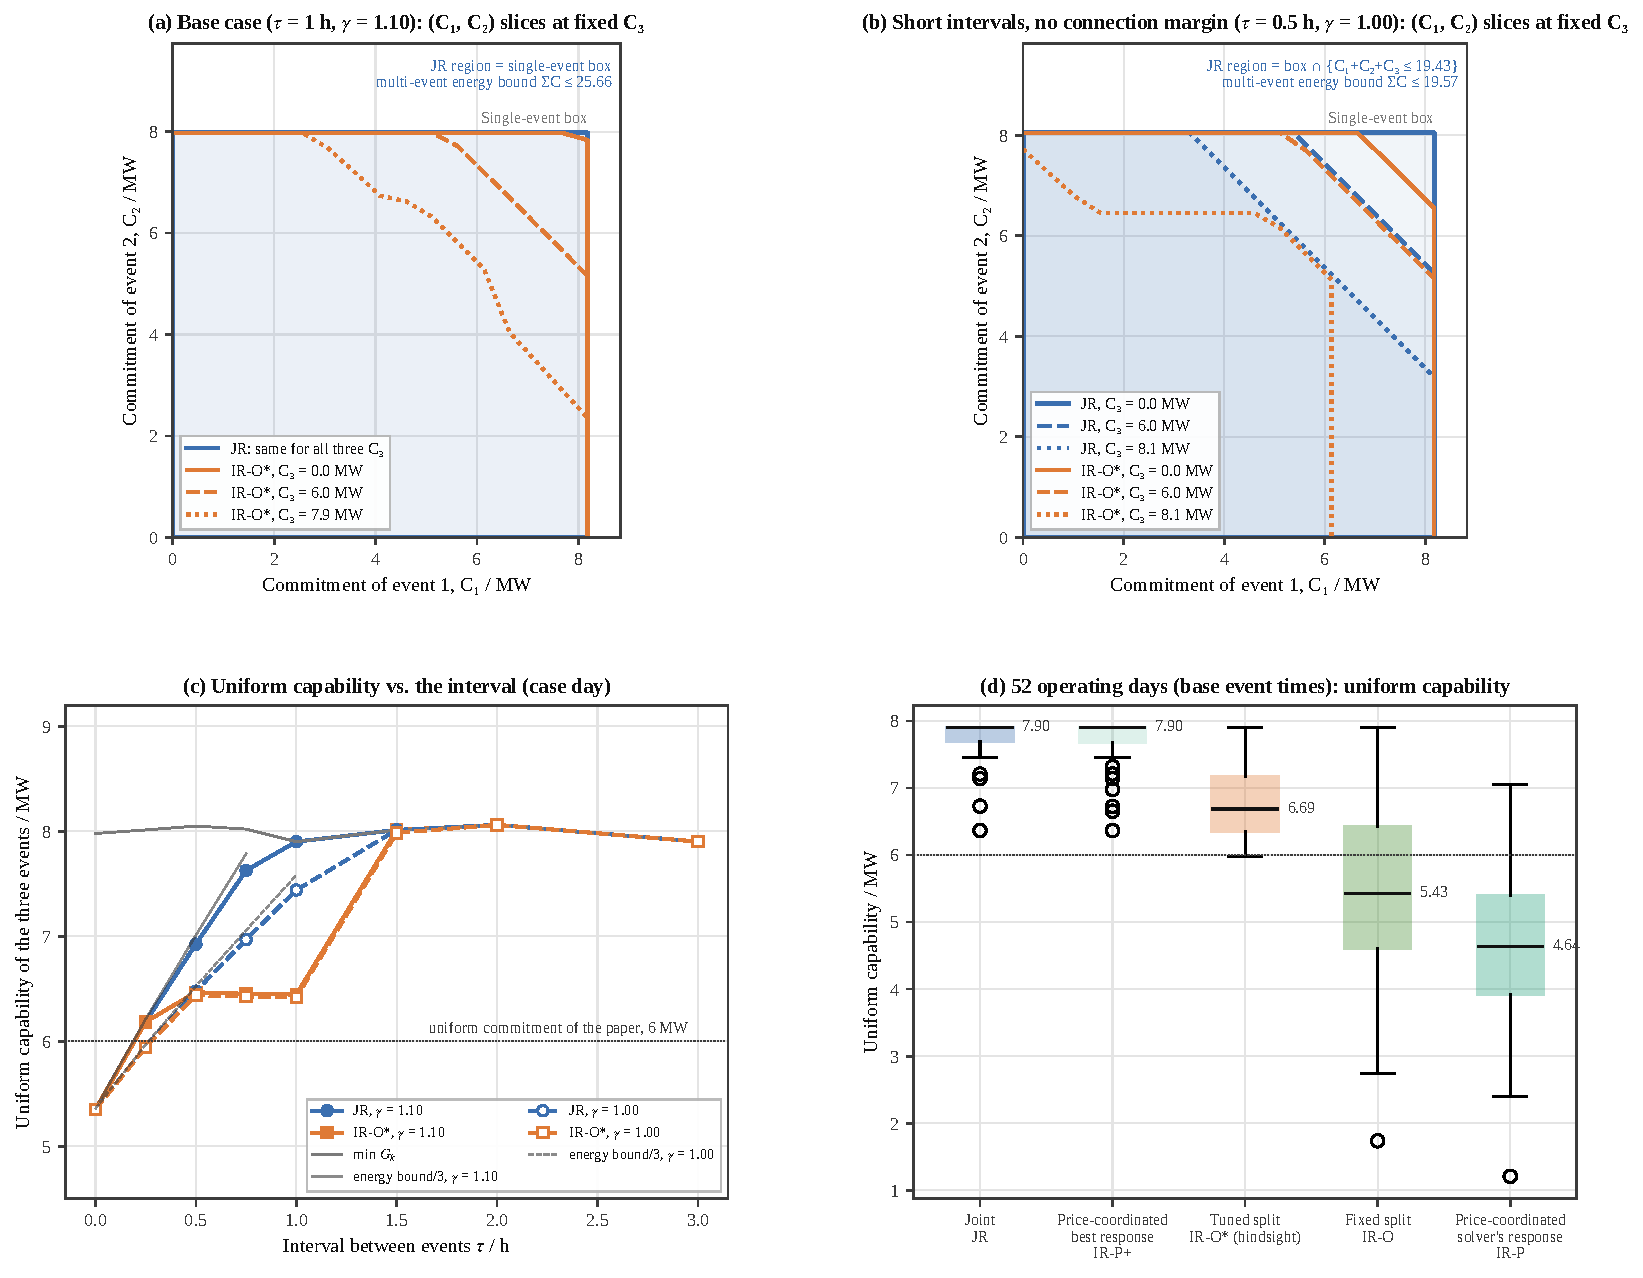
\includegraphics[width=0.86\textwidth]{fig28_region.pdf}
\caption{Cross-event capability region (perfect information). (a)(b) Slices $(C_1,C_2)$ at fixed $C_3$: joint recovery
(shaded, exact by the vertex certificate), IR-O* with the hindsight-optimal split for every commitment vector (lines),
and the single-event box (grey); (c) uniform capability of the three events versus the gap ($\gamma=1.10$ solid, $1.00$
dashed) with the minimum stand-alone capability and one third of the energy bound; (d) uniform capability on the 52
operating days, where IR-P+ is the most favourable and IR-P the solver's response to the price.}
\label{fig:region}
\end{figure*}

The capability region of joint recovery is the single-event box intersected with one total-energy cut. In both cases,
the support of every pair of events equals the sum of their stand-alone capabilities, so two events never conflict;
only the total of the three events can fall below the sum, which gives the single coupling cut $C_1+C_2+C_3\le h_{123}$
(each event lasts 1~h). In the base case, $h_{123}$ equals the sum of the stand-alone capabilities and the region is the
box itself, so the three events are independent; in the tight case the cut removes a corner of the box. This is the
virtual battery of Proposition~\ref{prop:region}: event power limits $\Gamma^0_k$ and one cross-event energy budget
$h_{123}$. All eight vertices of the template are deliverable in the base case, so the description is exact; in the
tight case one vertex falls marginally short ($\theta^*=0.9997$), \ie\ the template differs from the true region by
less than 0.03\%.

The multi-event energy bound is tight: it holds in all 24 gap--margin cases and on all 52 days, and where the cut is
active (14 cases and 18 days) it exceeds the exact LP value by 0.02--0.71~MWh ($\le$3.0\%). On the case day the evening load
without response and storage actions exceeds the baseline by about 2.2~MW, so the baseline difference $\Delta$ of the three events
is $-6.2$ to $-6.7$~MWh for gaps up to 1~h, a non-negligible part of the budget that the unbiased-baseline assumption
of Proposition~\ref{prop:bound} would ignore (the bound would overestimate by 42\% at a zero gap).

Independent recovery shrinks the cross-event energy budget rather than the stand-alone capabilities. In the base case
IR-O* reaches the JR boundary in every single-event and two-event direction, and the loss concentrates in the corner
where all three commitments are high: the maximum total commitment along the same rays is 19.33 against 23.70~MW
($-18.4\%$) and the uniform capability 6.44 against 7.90~MW ($-18.4\%$), although the volume is only 3.4\% smaller. The
fixed split IR-O loses more (volume $-23\%$, uniform capability 5.50~MW). In the tight case the channel is narrow
anyway and IR-O* nearly coincides with JR (Corollary~\ref{cor:novalue}(c)), but in directions with only two committed
events it still loses up to 11\%.

A price signal alone is not enough. The optimal IT response to the channel price is not unique, and the response
picked by the solver (IR-P) delivers only 53--82\% of JR along the rays of the base case (28\% of the volume) and 60\%
of the uniform capability of JR on average over the 52 days. Selecting the most favourable exactly optimal response
(IR-P+) reaches the JR boundary on all rays of the base case but only on 59\% of the rays of the tight case; with
$\gamma=1.00$ and gaps of 1.5--3~h no exactly optimal response is deliverable (uniform capability 4.97--5.72~MW against
7.90--8.06~MW for JR). Allowing the IT side to be 0.1\% suboptimal recovers the JR capability in all 24 cases and on all
52 days, except for up to 5\% in some directions of the tight case; the residual gap arises because the IT model
estimates its power budget with idle storage and converts cooling with the electric-chiller COP, so the joint price is
only an approximate supporting price for it. The channel price thus contains almost all the information needed but
does not select a deliverable plan: the IT side must also know which of its many near-optimal plans to choose.

The uniform capability of JR increases almost linearly with the gap and follows the energy bound
(\figref{fig:region}(c)). At a zero gap, JR, IR-O* and IR-P+ coincide (5.35~MW), since nothing can be recovered between
the events. JR reaches the stand-alone capability at a gap of 1~h with $\gamma=1.10$ and 1.5~h with $\gamma=1.00$; at a
gap of 1~h its uniform capability is 7.44/7.88/7.90~MW for $\gamma$ = 1.00/1.05/1.10. IR-O* stays at about 6.4~MW for gaps
of 0.5--1~h, because it spends the channel on unnecessary catch-up, and catches up with JR only from 1.5~h, which is the
difference of the minimum recovery gaps of Theorem~\ref{thm:closed} on the capability region. Over the 52 days the
uniform capability of JR averages 7.75~MW (6.37--7.90); relative to JR, IR-P+ achieves 99.4\%, IR-O* 88.6\% (80--100\%),
IR-O 71\% and IR-P 60\%, and the energy cut is active on 18 days.

For bidding, the current practice of one value per event requires the uniform capability to guarantee delivery under
any call pattern: 7.90~MW per event in the base case and 6.48~MW in the tight case. If the data center instead declares
the virtual-battery parameters (three $\Gamma^0_k$ and the budget $h_{123}$, four numbers), the grid operator may call
any combination within them; in the tight case, two calls of up to 8.0~MW each become possible, 24\% more than the
uniform declaration, while three calls may total at most 19.43~MW. Under independent recovery the same declaration
needs a further discount: the energy budget of IR-O* is 18\% lower than that of JR in the base case.

\subsubsection{Distributed coordination by plan--price exchange}
\label{sec:res-admm}

The previous subsection showed that a one-shot channel price does not determine a deliverable plan. Experiment~26 lets
the IT scheduler and the facility controller keep their own models, states and forecasts and exchange only the
deferrable power plan (one number per step) and the price, iterating \eqref{eq:admm} on the same joint model
(Proposition~\ref{prop:admm}); the facility side requires every called event to be valid and $\rho=200$~CNY per
MW$^2$ and step unless stated otherwise (\figref{fig:admm}).

\begin{figure*}[!t]
\centering
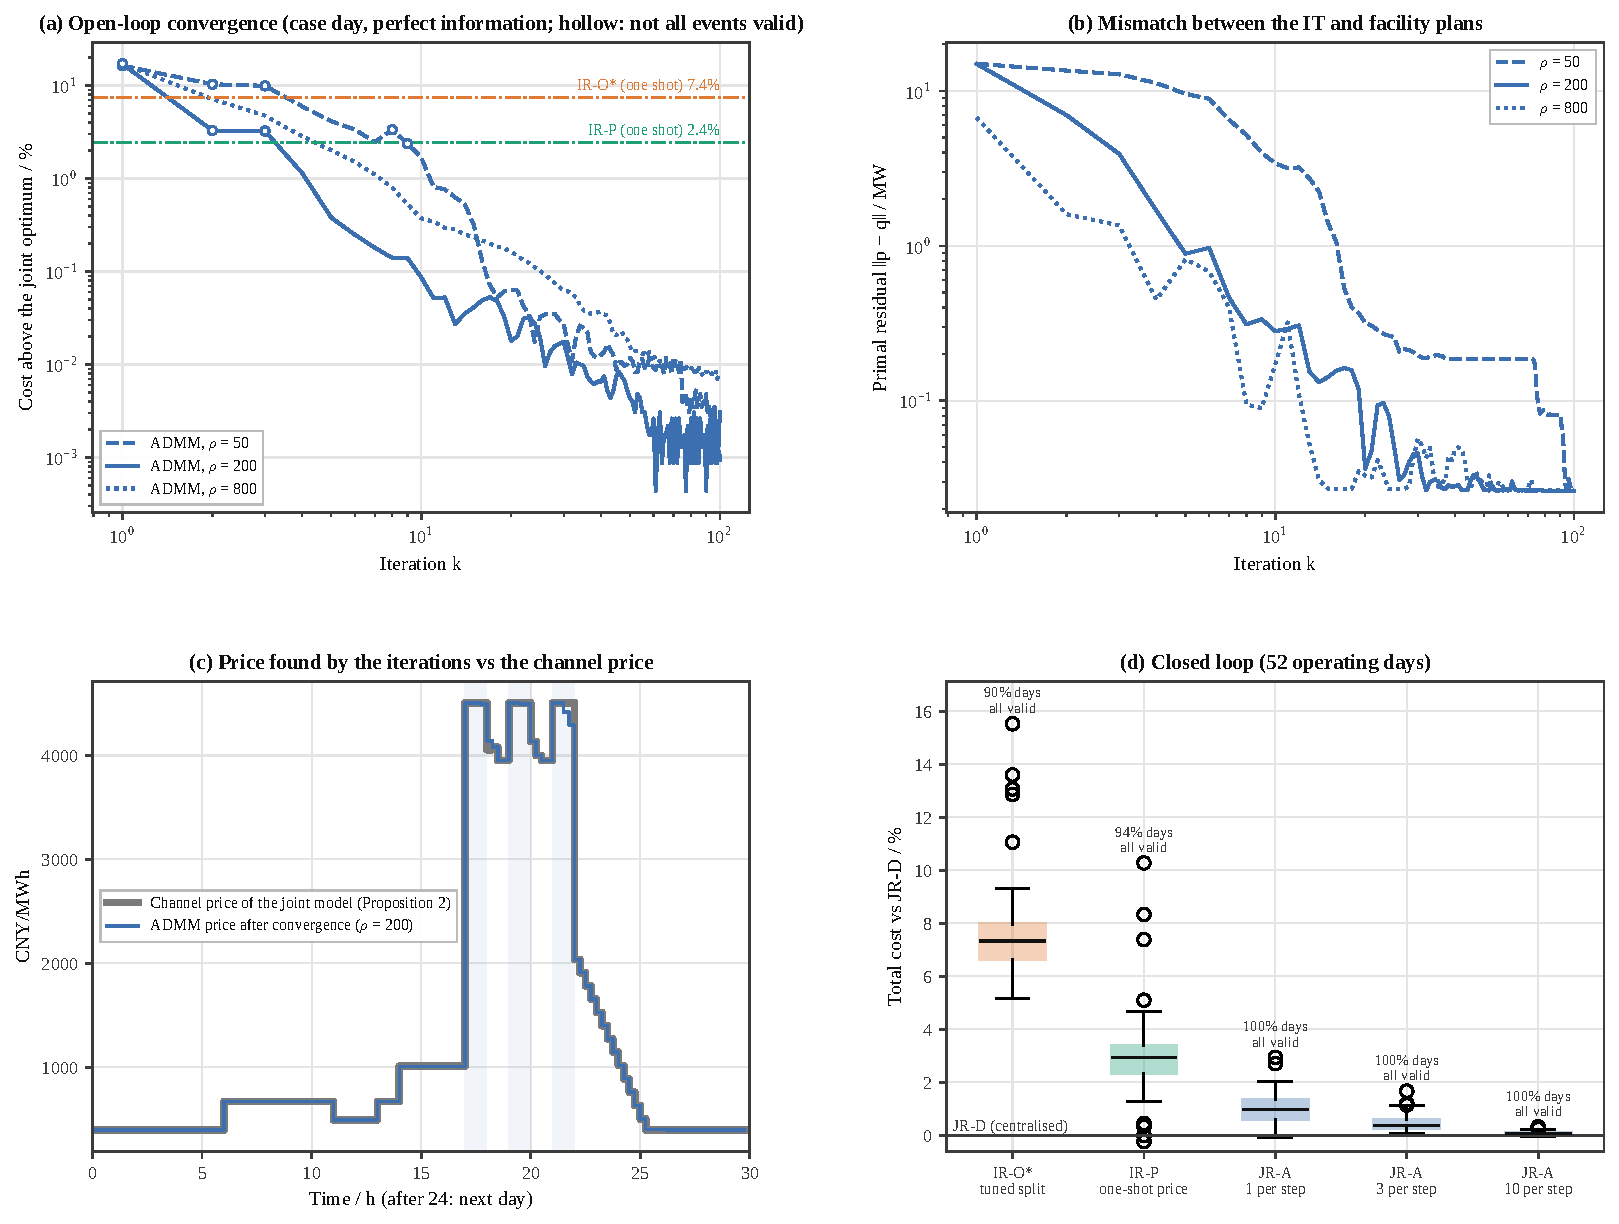
\includegraphics[width=0.86\textwidth]{fig29_admm.pdf}
\caption{Distributed joint recovery by plan--price exchange. (a) Open-loop cost of implementing the IT side's plan
relative to the joint optimum (log--log; hollow: not all events valid), with the one-shot benchmarks IR-P and IR-O*;
(b) mismatch between the two plans; (c) price after convergence ($\rho=200$) and channel price of the joint model
(shaded: events); (d) closed-loop cost relative to the centralised JR-D on 52 operating days and share of days with all
events valid.}
\label{fig:admm}
\end{figure*}

In open loop (case day, perfect information, uniform 6~MW), the relevant measure is the cost of implementing the IT
side's current plan, \ie\ the total cost when the facility responds optimally to it. With $\rho=200$ this cost falls
below that of the one-shot price coordination IR-P (2.44\% above the joint optimum) from the fourth iteration on, and
lies 0.38\%, 0.09\% and 0.02\% above the optimum after 5, 10 and 20 iterations; IR-O* with the hindsight-optimal split
is 7.38\% above. The iteration starts from the nominal IT load, and the IT plans of the first three iterations do not yet
keep all events valid: a few exchanges are needed to move catch-up out of the scarce hours. A small $\rho$ updates the
price slowly ($\rho=50$: better than IR-P from iteration 10, within 0.1\% from iteration 17), and a large one locks
the plans early ($\rho=800$: iterations 5 and 26). After 100 iterations the residual stays at about 0.03~MW, the
resolution of the tangent cuts, and the implemented cost is within 0.001--0.008\% of the optimum.

The price found by the iteration is the channel price (\figref{fig:admm}(c)). After convergence it differs from the
channel price of the joint model (Proposition~\ref{prop:price}) by less than 1~CNY/MWh in 79\% of the steps, and it
reproduces the price of about 4,500~CNY/MWh during the events and its gradual decline afterwards; only three steps at
the beginning and end of the events differ more (up to 214~CNY/MWh). The iteration discovers the channel price without
any party solving the joint model and broadcasting it.

In closed loop, the centralised JR-D costs $22.84\times10^4$~CNY on the case day, and JR-A with 1, 3 and 10 iterations
per MPC step costs $+0.67\%$, $+0.22\%$ and $+0.03\%$ more; with three iterations, $\rho$ = 50, 200 and 800 differ by
less than 0.1\%. Over the 52 days, JR-A costs $+0.99\%$, $+0.45\%$ and $+0.09\%$ more than JR-D with 1, 3 and 10
iterations and keeps all events valid on every day, whereas IR-P costs $+2.97\%$ more (all events valid on 94\% of the
days). One exchange per step thus recovers 67\% of the advantage of joint recovery over the strongest independent
benchmark, three exchanges 85\% and ten 97\%. A full day takes about 6~s for JR-D and 12/29/88~s for JR-A with
1/3/10 iterations, less than 1~s per step. Joint recovery therefore does not require merging the IT scheduler and the
facility energy management system: both keep their own models and data, provided that plans and prices are exchanged in
both directions a few times per 15~min.

\subsection{Day-ahead commitment under uncertainty}
\label{sec:res-dayahead}

\subsubsection{Commitment--operation pairing}
\label{sec:res-pairing}

Three commitments are compared on the case day and 20 operating days, each operated by IR-O* (with $\alpha$ re-tuned
for that commitment) and by JR-D: the single-event capability assessment (SE), the SE commitment scaled by the
back-tested factor $\theta^*=0.8$ (SE-$\theta$, a cautious conventional practice), and the coupled day-ahead commitment
(DA) (\tabref{tab:pairing}, \figref{fig:pairing}).

\begin{table}[!t]
\caption{Commitment--operation pairing (20 operating days): fulfilment / days with all events valid / mean cost
($10^4$~CNY).}
\label{tab:pairing}
\centering\footnotesize
\setlength{\tabcolsep}{2.8pt}
\begin{tabular}{@{}llcc@{}}
\toprule
Commitment (sum, MW) & Setting & IR-O* & \textbf{JR-D}\\
\midrule
SE 8.18/7.98/7.90 (24.1) & $\crb=3$ & 81.8\% / 45\% / 25.63 & 96.0\% / 95\% / 23.06\\
SE-$\theta$ 6.54/6.38/6.32 (19.2) & $\crb=3$ & 97.5\% / 95\% / 24.08 & 99.9\% / 100\% / 22.44\\
DA 3.27/6.65/7.90 (17.8) & $\crb=3$ & 97.0\% / 100\% / 23.79 & \textbf{98.8\% / 100\% / 22.39}\\
SE = DA 8.18/7.98/7.90 & $\crb=0$ & 84.3\% / 45\% / 21.43 & 96.0\% / 95\% / 19.18\\
SE-$\theta$ 6.54/6.38/6.32 & $\crb=0$ & 98.2\% / 95\% / 19.60 & \textbf{99.7\% / 100\% / 18.85}\\
\bottomrule
\end{tabular}
\end{table}

\begin{figure*}[!t]
\centering
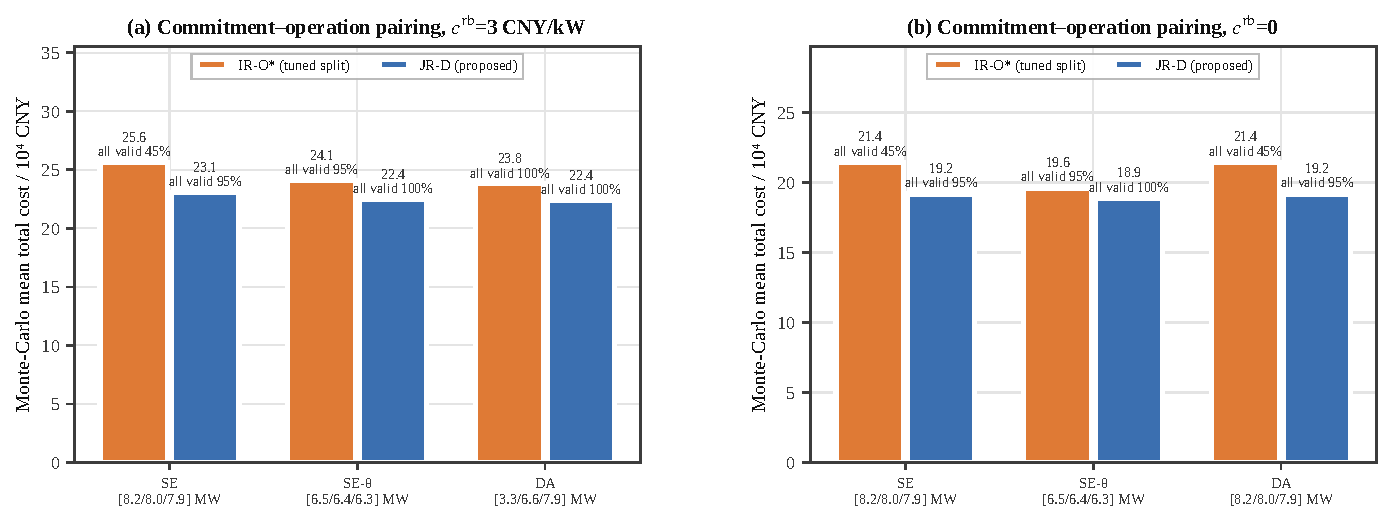
\includegraphics[width=0.86\textwidth]{fig09_commitment.pdf}
\caption{Commitment--operation pairing: mean total cost over 20 operating days with the share of days on which all
three events are valid.}
\label{fig:pairing}
\end{figure*}

The current practice, a single-event assessment operated by independent recovery (SE with IR-O*), keeps all three events
valid on only 45\% of the days. The coupled commitment operated by joint recovery (DA with JR-D) keeps them valid on
every day at a 12.6\% lower cost. Changing only the commitment to DA reduces the cost by 7.2\% (DA with IR-O*), and
operating the DA commitment by JR-D reduces it by a further 5.9\%. In the rebound-priced setting the coupled model
commits less in E1 and keeps the channel for the better-paid E3. In the rule setting the coupled commitment coincides
with the single-event capabilities, and the scaled SE-$\theta$ commitment is better for both operating strategies
because the five day-ahead scenarios cover the high-load tail of the operating days poorly; the risk-averse commitment
below addresses this.

\subsubsection{Risk-averse commitments}
\label{sec:res-risk}

Using ten historical joint scenarios and $\crb=3$, each risk setting of Proposition~\ref{prop:dro} yields a set of
commitments, which JR-D then operates out of sample on the same 52 days (\tabref{tab:risk}, \figref{fig:risk}).

\begin{table}[!t]
\caption{Risk-averse day-ahead commitments evaluated out of sample by JR-D on 52 days.}
\label{tab:risk}
\centering\footnotesize
\setlength{\tabcolsep}{2.8pt}
\begin{tabular}{@{}lcccc@{}}
\toprule
Setting & \makecell{E1/E2/E3 (sum)\\(MW)} & \makecell{Mean\\($10^4$~CNY)} & \makecell{Worst 10\%\\($10^4$~CNY)} & All valid\\
\midrule
SP ($\delta=0$) & 3.66/6.34/7.90 (17.9) & 22.50 & 27.33 & 100\%\\
DRO $\delta=0.2$ & 2.66/6.01/7.90 (16.6) & 22.47 & 27.27 & 100\%\\
DRO $\delta=0.4$ & 2.80/5.06/7.90 (15.8) & 22.45 & 27.24 & 100\%\\
\textbf{DRO $\delta=1.2$} & 0.96/5.77/7.90 (14.6) & \textbf{22.44} & \textbf{27.22} & 100\%\\
RO ($\delta=2$) & 4.54/2.17/7.90 (14.6) & 22.45 & 27.22 & 100\%\\
CVaR$_{0.8}$ & 4.22/2.50/7.90 (14.6) & 22.45 & 27.22 & 100\%\\
Mean--CVaR$_{0.9}$ ($w=0.5$) & 2.74/5.50/7.90 (16.1) & 22.46 & 27.26 & 100\%\\
Single-event assessment & 8.18/7.98/7.90 (24.1) & 23.11 & 29.12 & 96.2\%\\
\bottomrule
\end{tabular}
\end{table}

\begin{figure*}[!t]
\centering
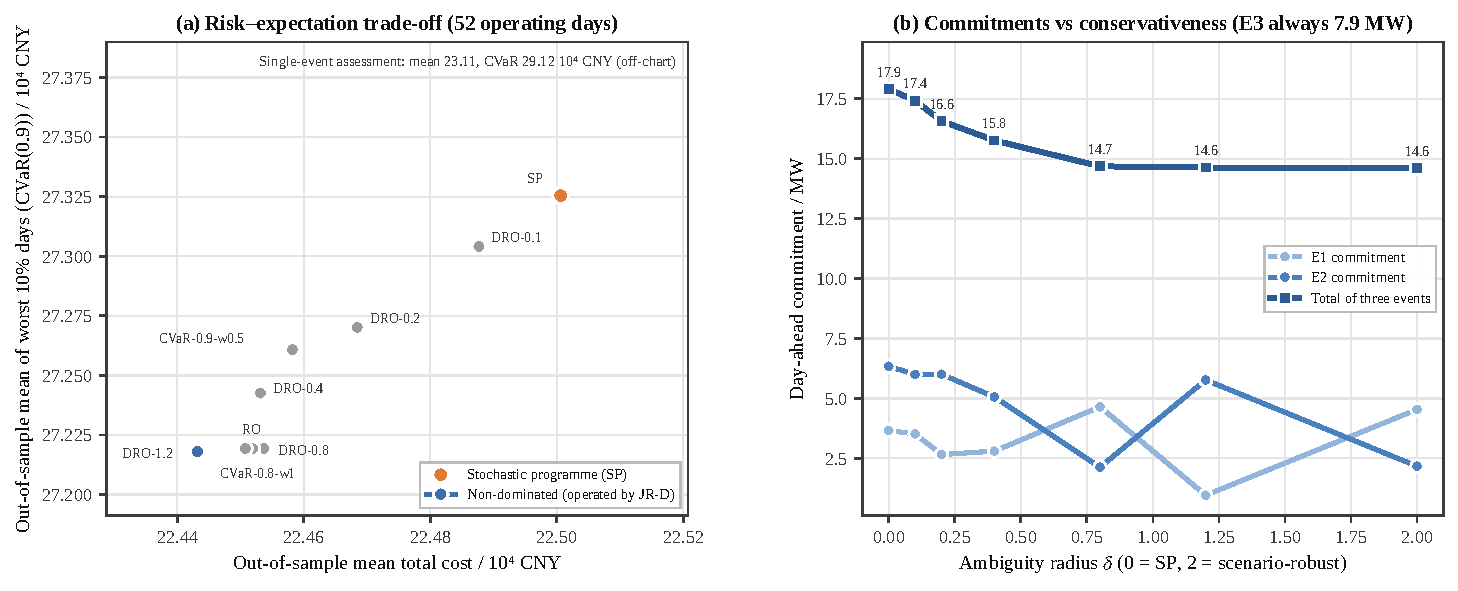
\includegraphics[width=0.86\textwidth]{fig15_risk_pareto.pdf}
\caption{Risk-averse commitments. (a) Out-of-sample mean and mean of the worst 10\% of days for each risk setting on the
52 days (the single-event assessment lies outside the chart); (b) commitments versus the ambiguity radius $\delta$.}
\label{fig:risk}
\end{figure*}

A higher conservativeness lowers the total commitment: as $\delta$ increases from 0 to 0.8, the sum falls monotonically
from 17.9 to 14.7~MW and then stays constant. The best-paid E3 is always committed at its capability of 7.9~MW and the
reduction falls on E1 and E2, between which the model is nearly indifferent, so their split is not unique
(\figref{fig:risk}(b)). The distributionally robust commitments lower both the mean and the tail out of sample: compared
with SP, $\delta$ = 0.4--1.2 reduces the mean by 0.21--0.26\% and the mean of the worst 10\% of days by 0.3--0.4\%, all
paired differences being significant (Wilcoxon $p\le2\times10^{-4}$). $\delta=1.2$ is best in both measures and is the
non-dominated knee point of \figref{fig:risk}(a). The reason is that the ten historical scenarios cover the high-load tail
of the operating days poorly, so SP commits too much and earns less and pays more on adverse days, which the robust
commitments avoid by committing less in E1 and E2. The improvement is small, which shows that coupled commitment with
joint recovery is already robust. Coupled commitments are far better than the single-event assessment, which costs 2.7\%
more on average and 6.6\% more on the worst 10\% of days, with all events valid on only 96.2\% of the days. The DRO
model adds only 21 continuous variables and 30 constraints and solves in 14--25~s with ten scenarios, against 10~s for SP.

\subsubsection{Scenario generation and seasonal drift}
\label{sec:res-scen}

The base commitment uses five equally likely quantile scenarios. Experiment~23 replaces them by K-means scenarios with
non-uniform probabilities ($K$ = 5, 10, 20) and builds a DRO ball with $\delta=0.4$ around them; JR-D then operates each
commitment on the 52 out-of-sample days (\tabref{tab:scen}, \figref{fig:ext}(b)--(d)).

\begin{table}[!t]
\caption{Scenario generation: commitments and costs (52 days, operated by JR-D; costs in $10^4$~CNY).}
\label{tab:scen}
\centering\footnotesize
\setlength{\tabcolsep}{2.4pt}
\begin{tabular}{@{}lccccc@{}}
\toprule
Scenarios & \makecell{E1/E2/E3\\(MW)} & \makecell{In-\\sample} & \makecell{Out-of-\\sample} & \makecell{vs\\quantile-5} & \makecell{In-sample\\underestimate}\\
\midrule
Quantile-5 & 3.27/6.65/7.90 & 19.92 & 22.50 & -- & 13.0\%\\
K-means-5 & 2.42/5.63/7.90 & 20.96 & 22.45 & $-0.19\%$ & 7.1\%\\
K-means-10 & 3.69/4.72/7.90 & 20.68 & 22.46 & $-0.15\%$ & 8.6\%\\
K-means-20 & 3.73/5.51/7.90 & 20.22 & 22.48 & $-0.07\%$ & 11.2\%\\
K-means-5 + DRO & 0.92/6.32/7.90 & 21.10 & 22.45 & $-0.23\%$ & 6.4\%\\
K-means-10 + DRO & 4.71/2.99/7.90 & 20.86 & 22.46 & $-0.19\%$ & 7.6\%\\
\bottomrule
\end{tabular}
\end{table}

\begin{figure*}[!t]
\centering
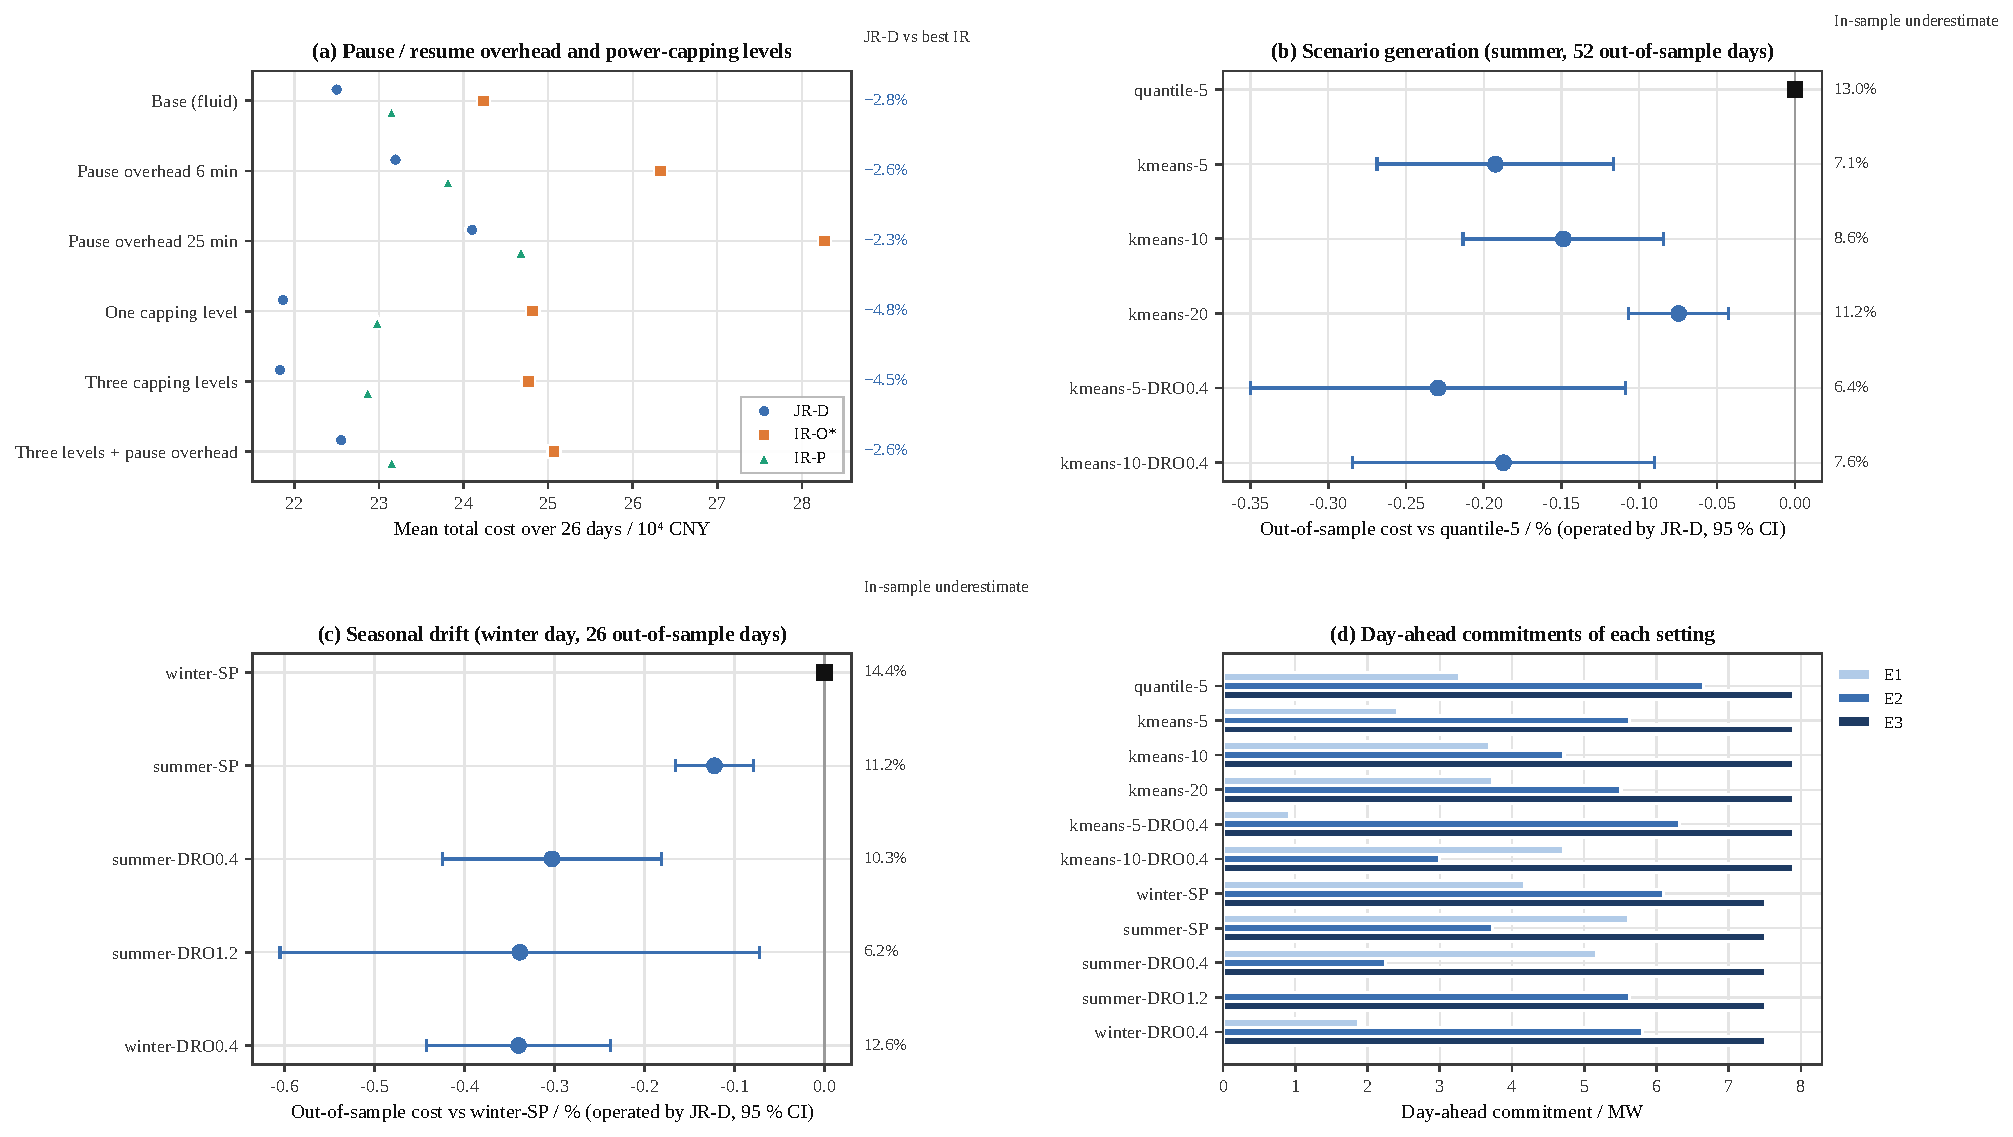
\includegraphics[width=0.96\textwidth]{fig25_extensions.pdf}
\caption{(a) Pause/resume overheads and power-capping levels: mean total cost on 26 operating days (right: JR-D relative
to the strongest independent benchmark); (b)(c) scenario generation and seasonal drift: paired out-of-sample cost
difference to the reference setting (95\% CI; right: underestimate of the in-sample estimate); (d) day-ahead
commitments of each setting.}
\label{fig:ext}
\end{figure*}

The out-of-sample cost is nearly insensitive to scenario generation: the six settings differ by less than 0.23\% and
keep all events valid on every day, although the commitments differ widely (E1 from 0.9 to 4.7~MW, E2 from 3.0 to
6.7~MW). The cost is therefore flat around the optimal commitment, consistent with \secref{sec:res-risk}; the K-means
improvements are statistically significant (Wilcoxon $p\le3\times10^{-5}$) but negligible in size. In-sample estimates
are optimistic by 6--13\%, mainly because the day-ahead model optimises each scenario with perfect information whereas the
operation has only forecasts; K-means-5/10 and DRO reduce the bias to 6--9\%, but 20 scenarios raise it again to 11\%.
Revenue estimates for bidding and investment appraisals should therefore rely on the out-of-sample cost of rolling
operation. A seasonal drift matters little: when the winter case day (10 January 2025) builds its scenarios from the
summer weather pool instead of the winter pool, the commitments change markedly (\figref{fig:ext}(d)) but the cost on 26
out-of-sample winter days is 0.12\% lower rather than higher, with all events valid every day, and DRO with
$\delta$ = 0.4/1.2 lowers it consistently by about 0.3\%.

\subsection{Sensitivity analysis}
\label{sec:res-sens}

To evaluate the robustness of the conclusions under different operating conditions and policy settings, this subsection
varies the commitment and system margins, the settlement and policy parameters, the realism of the model and the
external conditions.

\subsubsection{Commitment level, event gap and connection margin}
\label{sec:sens-commit}

Under perfect information, with IR-O* using the hindsight-optimal split and IR-P the perfect-information shadow price,
\figref{fig:sens} varies the event duration, gap, connection margin and commitment, and \figref{fig:map} maps the cost
reduction on the gap--margin plane; \tabref{tab:sens} lists the commitment sweep.

\begin{table}[!t]
\caption{Commitment sweep under perfect information: fulfilment / total cost ($10^4$~CNY).}
\label{tab:sens}
\centering\footnotesize
\setlength{\tabcolsep}{3pt}
\begin{tabular}{@{}llcccc@{}}
\toprule
Commitment & Setting & IR-O* (hindsight) & IR-P & \textbf{JR} & JR vs best\\
\midrule
6~MW & $\crb=0$ & 100\% / 19.91 & 100\% / 19.92 & 100\% / 19.31 & $-3.0\%$\\
7~MW & $\crb=0$ & 92.1\% / 20.43 & 88.8\% / 20.60 & \textbf{100\% / 19.04} & $-6.8\%$\\
8~MW & $\crb=0$ & 79.8\% / 22.27 & 77.7\% / 22.23 & \textbf{99.5\% / 19.09} & $-14.1\%$\\
9~MW & $\crb=0$ & 71.6\% / 23.23 & 69.0\% / 23.25 & 89.1\% / 20.06 & $-13.7\%$\\
8~MW & $\crb=3$ & 74.5\% / 26.76 & 92.9\% / 24.07 & \textbf{99.5\% / 23.09} & $-4.1\%$\\
\bottomrule
\end{tabular}
\end{table}

\begin{figure*}[!t]
\centering
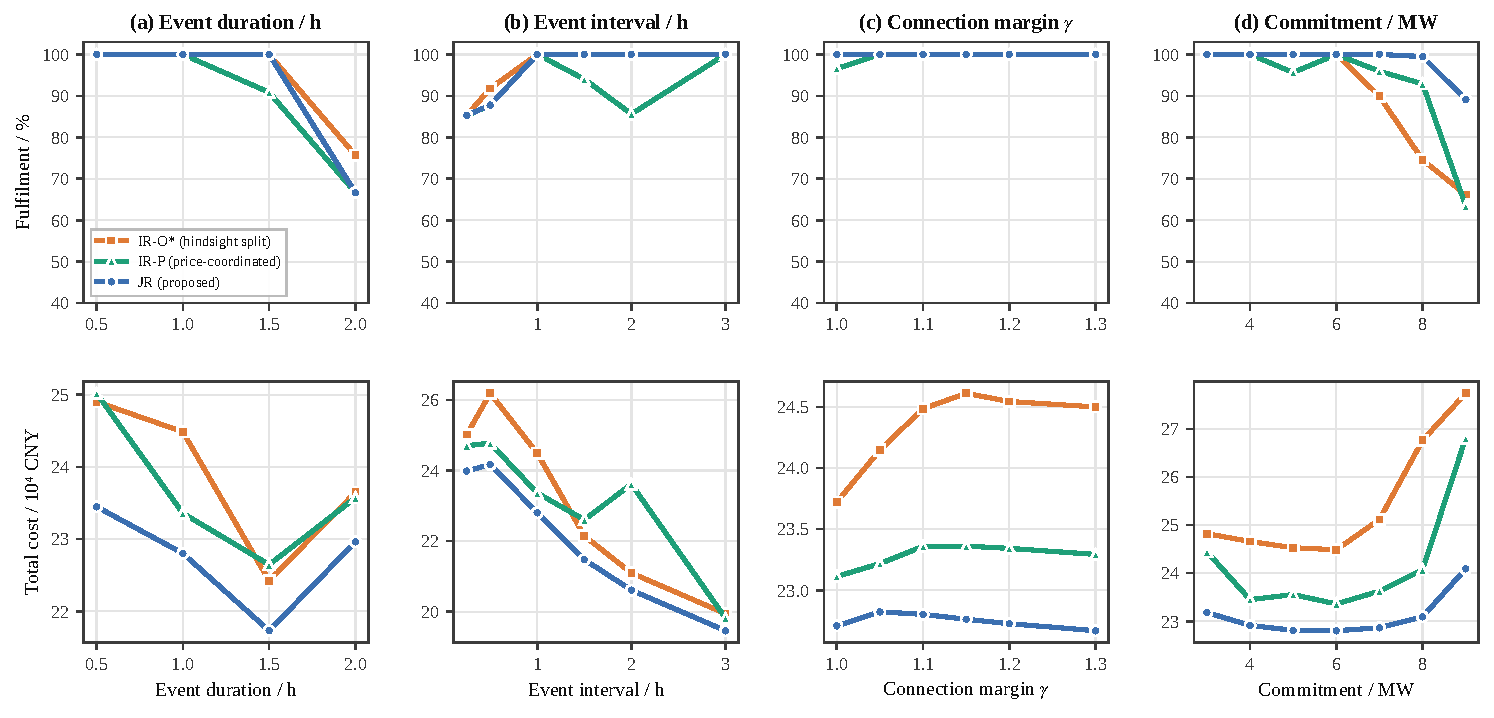
\includegraphics[width=0.96\textwidth]{fig05_sensitivity.pdf}
\caption{Sensitivity under perfect information ($\crb=3$~CNY/kW): fulfilment (top) and total cost (bottom) versus (a)
event duration, (b) event gap, (c) connection margin and (d) uniform commitment. The rule setting is shown in
\figref{fig:sens0}.}
\label{fig:sens}
\end{figure*}

\begin{figure*}[!t]
\centering
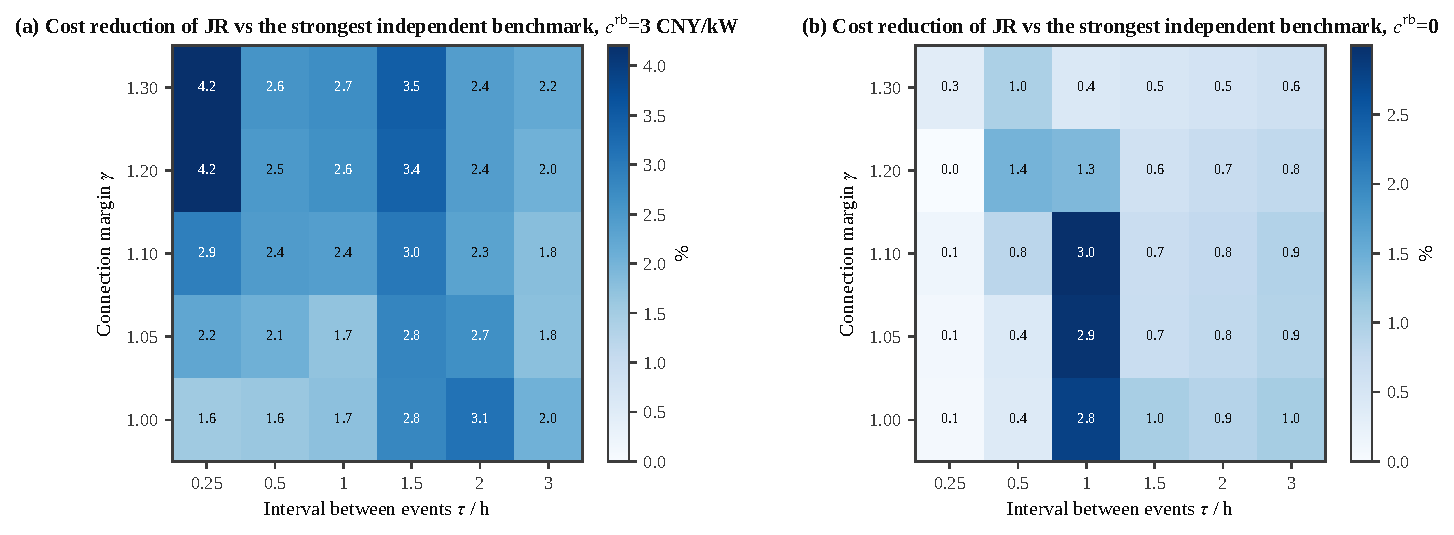
\includegraphics[width=0.94\textwidth]{fig06_interval_capacity_map.pdf}
\caption{Cost reduction of JR relative to the stronger of IR-O* and IR-P on the gap--margin plane: (a) rebound-priced
setting, (b) rule setting.}
\label{fig:map}
\end{figure*}

Deliverable capacity is the main value of joint recovery. With the requirement of $\ge$99\% fulfilment, even
hindsight-tuned independent recovery can commit only about 6~MW per event, whereas JR can commit about 8~MW (+33\%); at
8~MW, JR fulfils 99.5\% against less than 80\% for the best benchmark in the rule setting, at a 14.1\% lower cost. With
moderate commitments (6~MW) the advantage is only 2--3\%. On the gap--margin plane the reduction in the rule setting is
0--3.0\%, with the peak at a gap of 1~h and $\gamma\le1.10$ (2.8--3.0\%) and generally at most 1.4\% for gaps of 0.5~h
or less or 1.5~h or more; in the rebound-priced setting it is 1.6--4.2\% and never negative. Corollary~\ref{cor:novalue}
explains why the advantage first rises and then falls with the channel width: with a too narrow channel neither strategy
recovers, with a wide one both do.

Fulfilment is not what joint recovery maximises. With a gap of 0.5~h and $\crb=3$, JR fulfils 4--6 points less than
IR-O* but at a lower cost: the optimum delivers slightly above the 80\% validity threshold in some events to reduce the
rebound charge. With 2-h events, all three methods keep only two events valid. Both effects are cross-event trade-offs
induced by the Jiangsu settlement (80\% threshold, 120\% cap). Correcting the IT budget of the benchmarks
(\secref{sec:strategies}) has little effect under perfect information: at 6~MW the costs of IR-O* and IR-P drop by only
$0.06$--$0.07\times10^4$~CNY and the capacity conclusions are unchanged; the correction matters mainly for closed-loop
operation on heavy-load days.

\subsubsection{Rebound charge and DR payment}
\label{sec:sens-rebound}

\tabref{tab:rebound} and \figref{fig:rebound} treat the rebound charge as a policy parameter (case day, uniform 6~MW,
deterministic rolling operation). As the charge rises, the maximum rebound of JR-D after the events falls smoothly from
6.52 to 2.98~MW, its fulfilment stays at 100\% up to 4~CNY/kW, and JR-D is the cheapest strategy at every charge. IR-P
cuts the rebound to 2.04~MW at 6~CNY/kW, but its fulfilment drops to 65.9\%. On the plane of cost (excluding the rebound
charge) against maximum rebound, the trade-off curve of JR-D lies to the lower left of the benchmarks
(\figref{fig:rebound}(a)): controlling the rebound while keeping the events valid requires a joint allocation of the
channel. Without a rebound charge, however, joint recovery does not suppress the rebound by itself, since all strategies
raise the import to near the connection limit; whether and at which price to charge rebound is a policy choice of the
grid operator or aggregator, and joint recovery minimises its cost.

\begin{table}[!t]
\caption{Rebound charge as a policy parameter (case day, uniform 6~MW).}
\label{tab:rebound}
\centering\footnotesize
\setlength{\tabcolsep}{3pt}
\begin{tabular}{@{}lccccccc@{}}
\toprule
$\crb$ (CNY/kW) & 0 & 0.5 & 1 & 2 & 3 & 4 & 6\\
\midrule
JR-D max rebound (MW) & 6.52 & 6.47 & 6.45 & 6.31 & 5.77 & 5.27 & 2.98\\
JR-D cost ($10^4$~CNY) & 19.34 & 20.12 & 20.83 & 22.02 & 22.84 & 23.47 & 24.47\\
Best benchmark ($10^4$~CNY) & 19.97 & 20.79 & 21.57 & 22.60 & 23.61 & 24.48 & 25.88\\
& \scriptsize IR-O* & \scriptsize IR-O* & \scriptsize IR-O* & \scriptsize IR-P & \scriptsize IR-P & \scriptsize IR-P & \scriptsize IR-P\\
JR-D vs best & $-3.2\%$ & $-3.3\%$ & $-3.4\%$ & $-2.6\%$ & $-3.3\%$ & $-4.1\%$ & $-5.5\%$\\
\bottomrule
\end{tabular}
\end{table}

\begin{figure*}[!t]
\centering
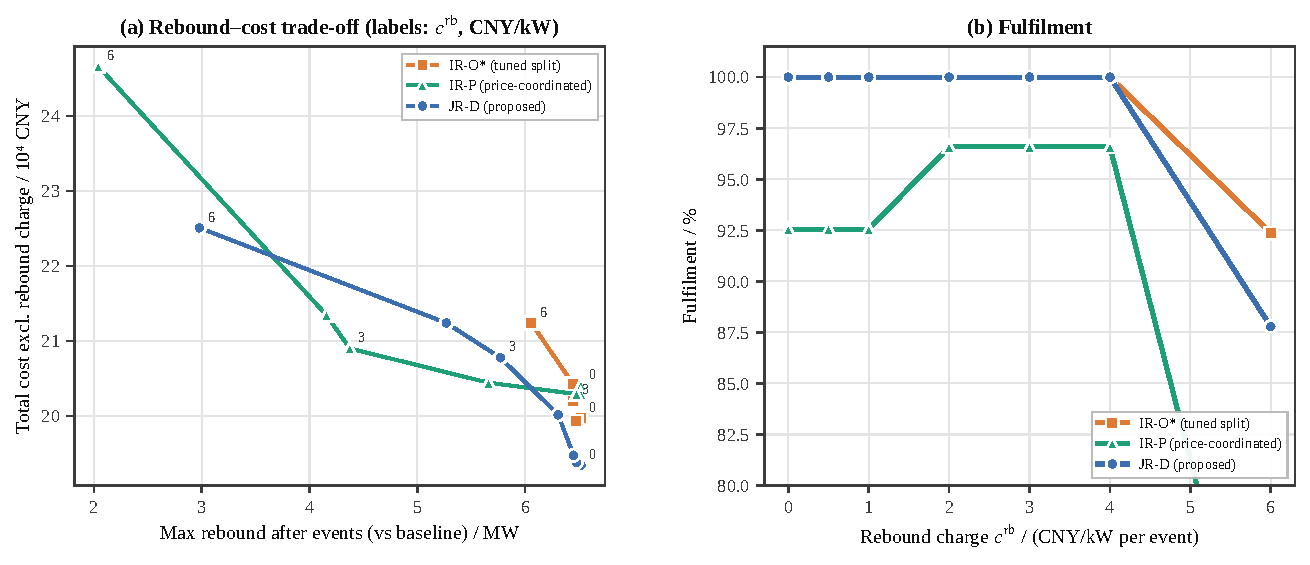
\includegraphics[width=0.84\textwidth]{fig10_rebound_pareto.pdf}
\caption{Rebound charge as a policy parameter. (a) Trade-off between the cost excluding the rebound charge and the
maximum rebound (labels: $\crb$ in CNY/kW); (b) fulfilment versus the rebound charge.}
\label{fig:rebound}
\end{figure*}

Across the nine combinations of DR payment (1--3~CNY/kWh) and shortfall coefficient ($\kappa$ = 0.5--2), JR-D is
always the cheapest, by 1.5\% (1~CNY/kWh, $\kappa=0.5$) to 4.0\% (3~CNY/kWh, $\kappa=2$) against the strongest benchmark
(\figref{fig:robust}(a)): the higher the payment and the stricter the shortfall assessment, the more valuable joint
recovery. At 1~CNY/kWh all three optimised strategies respond only partially (JR-D fulfils 33--88\%), since keeping
most events valid is no longer worthwhile.

\begin{figure*}[!t]
\centering
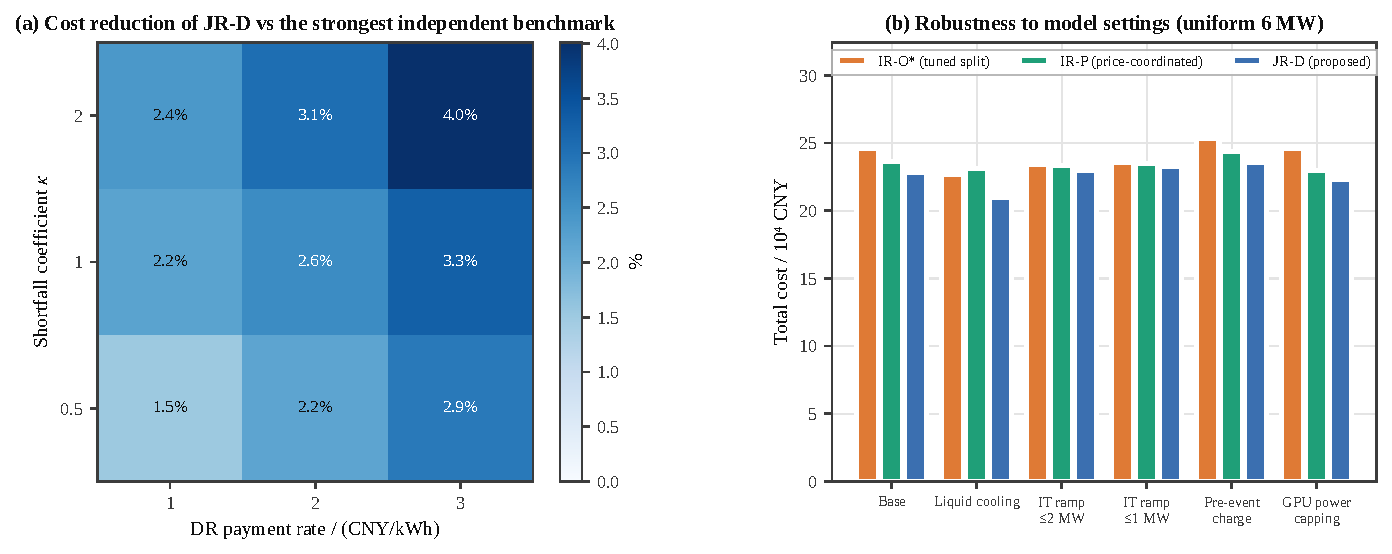
\includegraphics[width=0.90\textwidth]{fig13_robustness.pdf}
\caption{(a) Cost reduction of JR-D relative to the strongest independent benchmark for different DR payments and
shortfall coefficients; (b) total cost under different model settings (uniform 6~MW).}
\label{fig:robust}
\end{figure*}

\subsubsection{Realism, multi-energy coupling and policy constraints}
\label{sec:sens-real}

\tabref{tab:realism} and \figref{fig:robust}(b) add realistic features one at a time (uniform 6~MW, $\crb=3$,
deterministic rolling operation). Liquid cooling makes joint recovery more important: it lowers the cooling power, so the
connection limit, which follows the typical-day peak, falls to 14.59~MW and the channel narrows; IR-P then fulfils only
80.8\%, while JR-D still fulfils every event at a 7.4\% lower cost. IT ramp limits compress the room for joint recovery:
at 1~MW per 15~min the advantage shrinks to 0.8\%, because the ramp limit flattens the catch-up profile. A pre-event
load-up charge of 1,000~CNY/MWh adds the same amount to all strategies and does not change the schedule, since the
load-up stems from reserving storage for the events rather than from inflating the baseline. GPU power capping is an
effective additional lever: each unit of power reduction leaves only 0.4 units of debt, which lowers the cost of JR-D by
a further 2.4\% and its maximum rebound from 5.77 to 4.02~MW.

\begin{table}[!t]
\caption{Realism (uniform 6~MW, $\crb=3$): fulfilment / total cost ($10^4$~CNY).}
\label{tab:realism}
\centering\footnotesize
\setlength{\tabcolsep}{2.6pt}
\begin{tabular}{@{}lcccc@{}}
\toprule
Setting & IR-O* & IR-P & \textbf{JR-D} & JR-D vs best\\
\midrule
Base & 100\% / 24.57 & 96.6\% / 23.61 & \textbf{100\% / 22.84} & $-3.3\%$\\
Liquid cooling & 94.3\% / 22.66 & 80.8\% / 23.10 & \textbf{100\% / 20.98} & $-7.4\%$\\
IT ramp $\le$2~MW/15~min & 100\% / 23.45 & 98.1\% / 23.37 & \textbf{100\% / 22.98} & $-1.6\%$\\
IT ramp $\le$1~MW/15~min & 100\% / 23.56 & 95.5\% / 23.47 & \textbf{100\% / 23.29} & $-0.8\%$\\
Pre-event charge & 100\% / 25.31 & 96.6\% / 24.36 & \textbf{100\% / 23.59} & $-3.2\%$\\
GPU power capping & 92.0\% / 24.63 & 96.4\% / 22.94 & \textbf{100\% / 22.28} & $-2.9\%$\\
\bottomrule
\end{tabular}
\end{table}

\begin{figure*}[!t]
\centering
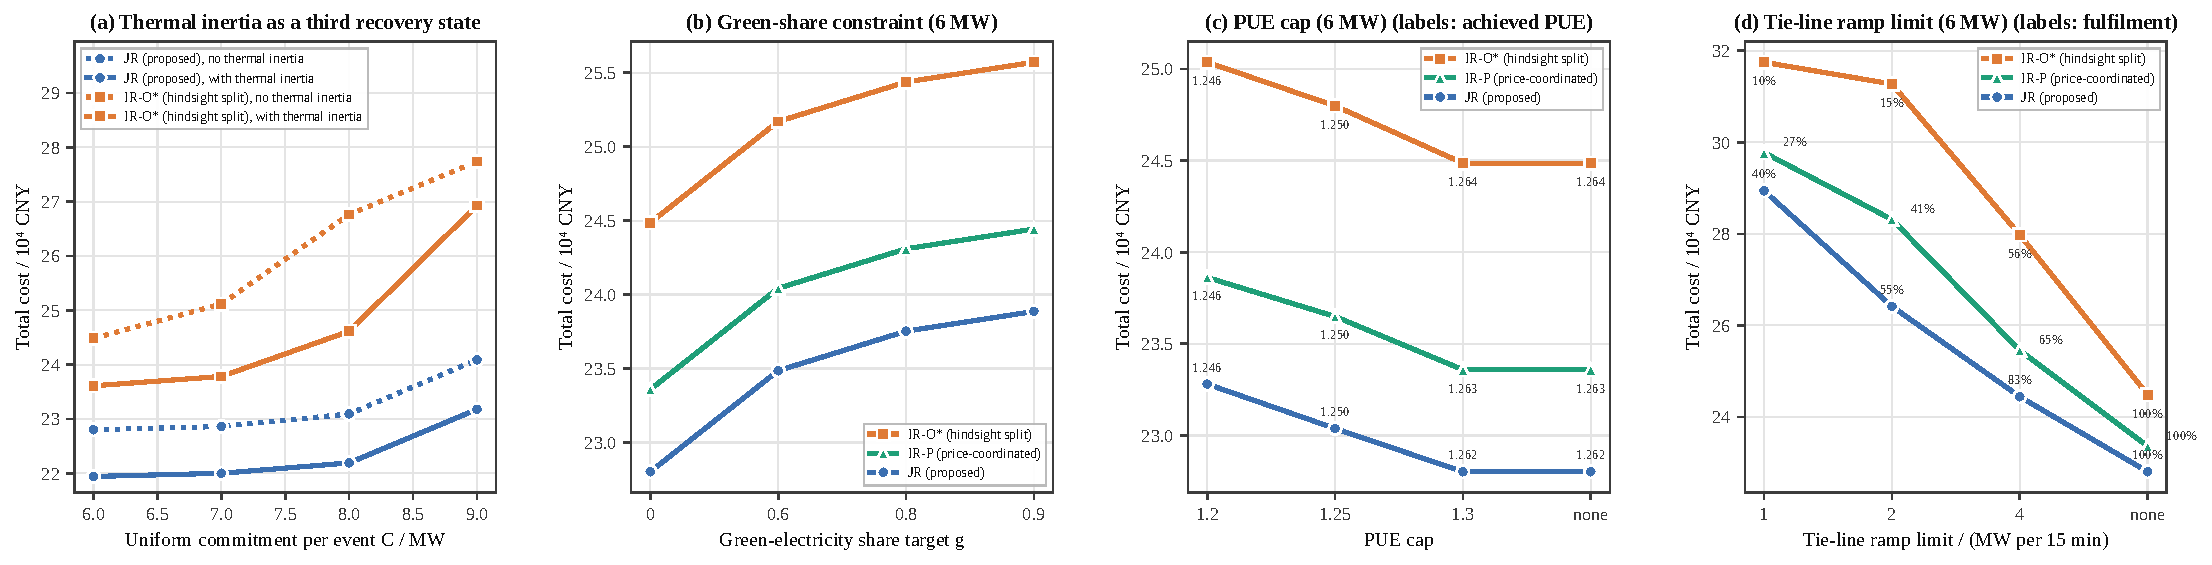
\includegraphics[width=\textwidth]{fig21_policy.pdf}
\caption{Multi-energy coupling and policy constraints ($\crb=3$, perfect information). (a) Data hall thermal inertia on
and off versus the commitment; (b) green-electricity share target; (c) PUE cap (labels: achieved PUE); (d) tie-line
ramp limit (labels: fulfilment).}
\label{fig:policy}
\end{figure*}

\figref{fig:policy} adds multi-energy coupling and policy constraints. Data hall thermal inertia acts as a third
recovery state: allowing the hall to float between $-2$ and $+3$~K around the set-point, all strategies use the full
3.0~K and save 0.86--0.88$\times10^4$~CNY per day (JR: 22.80 to 21.94), and in closed loop on 26 days JR-D saves 3.8\%
and IR-P 4.3\%. Thermal inertia is another free and fast storage that the facility side can use under independent
recovery too: at 8~MW the fulfilment of IR-P rises from 92.9\% to 99.4\%, level with JR (99.5\%). The advantage of joint
recovery remains but shrinks ($-2.6\%$ under perfect information at 8~MW, $-2.2\%$ in closed loop with
$p=1.5\times10^{-7}$), because more storage-side flexibility partly substitutes for joint recovery, as with large
batteries in \secref{sec:res-capacity}. Green-electricity targets of 60/80/90\% raise the daily cost of all strategies
by 0.68/0.95/1.08$\times10^4$~CNY with differences below 10~CNY between them, \ie\ in this accounting a green share acts
like a uniform surcharge on grid and gas electricity and does not change the ranking. Without a PUE cap, the PUE on the
DR day is 1.262--1.264; a cap of 1.25 is met by all strategies at an extra cost of 0.24 (JR) to 0.31 (IR-O*)
$\times10^4$~CNY by more absorption cooling, night-time TES charging and catch-up in cooler hours, whereas a cap of
1.20 is infeasible on this hot day (the minimum is 1.246, at 0.48--0.55$\times10^4$~CNY). Tie-line ramp limits of 4/2/1~MW
per 15~min directly restrict a fast load drop at the start of an event: the fulfilment of JR falls to
82.9/54.6/40.2\%, that of the benchmarks more (IR-P 64.9/41.2/27.2\%), and JR is 4.0/6.7/2.8\% cheaper than IR-P.
Without the limit, the largest step change of JR is a drop of 8.8~MW and a rise of 12.4~MW; since the Jiangsu rules judge
validity by the hourly mean, such ramp requirements would have to be designed together with the validity rule.

\subsubsection{Tariff shapes, seasons and climates}
\label{sec:sens-gen}

Five TOU shapes with the same daily mean are compared on 20 operating days (\figref{fig:gen}(a), \tabref{tab:tariff}).
The advantage of joint recovery is almost independent of the tariff shape: the cost reduction against IR-P is
2.1--2.9\% ($p\le4\times10^{-6}$), and the fulfilment of JR at 8~MW under perfect information is 99.5\% for every shape.
It is smallest under a flat tariff, where it matters less to which hours catch-up and recharging are moved.

\begin{table}[!t]
\caption{Tariff shapes (same daily mean): mean cost on 20 days ($10^4$~CNY) and fulfilment at 8~MW.}
\label{tab:tariff}
\centering\footnotesize
\setlength{\tabcolsep}{2.6pt}
\begin{tabular}{@{}lccc@{}}
\toprule
Tariff shape & \makecell{IR-O* / IR-P / JR-D} & \makecell{JR-D vs IR-P\\(paired)} & \makecell{8-MW fulfilment\\IR-O* / IR-P / JR}\\
\midrule
Jiangsu TOU (base) & 24.21 / 23.09 / 22.43 & $-2.86\%$ & 74.5 / 92.9 / 99.5\%\\
Flat & 27.94 / 27.08 / 26.51 & $-2.11\%$ & 74.5 / 93.0 / 99.5\%\\
Two-tier (peak 8--22~h) & 24.94 / 24.03 / 23.40 & $-2.61\%$ & 75.5 / 93.0 / 99.5\%\\
Critical peak (19--21~h) & 24.13 / 22.96 / 22.30 & $-2.85\%$ & 76.4 / 92.9 / 99.5\%\\
Duck curve & 25.20 / 24.22 / 23.53 & $-2.84\%$ & 69.3 / 92.9 / 99.5\%\\
\bottomrule
\end{tabular}
\end{table}

\begin{figure*}[!t]
\centering
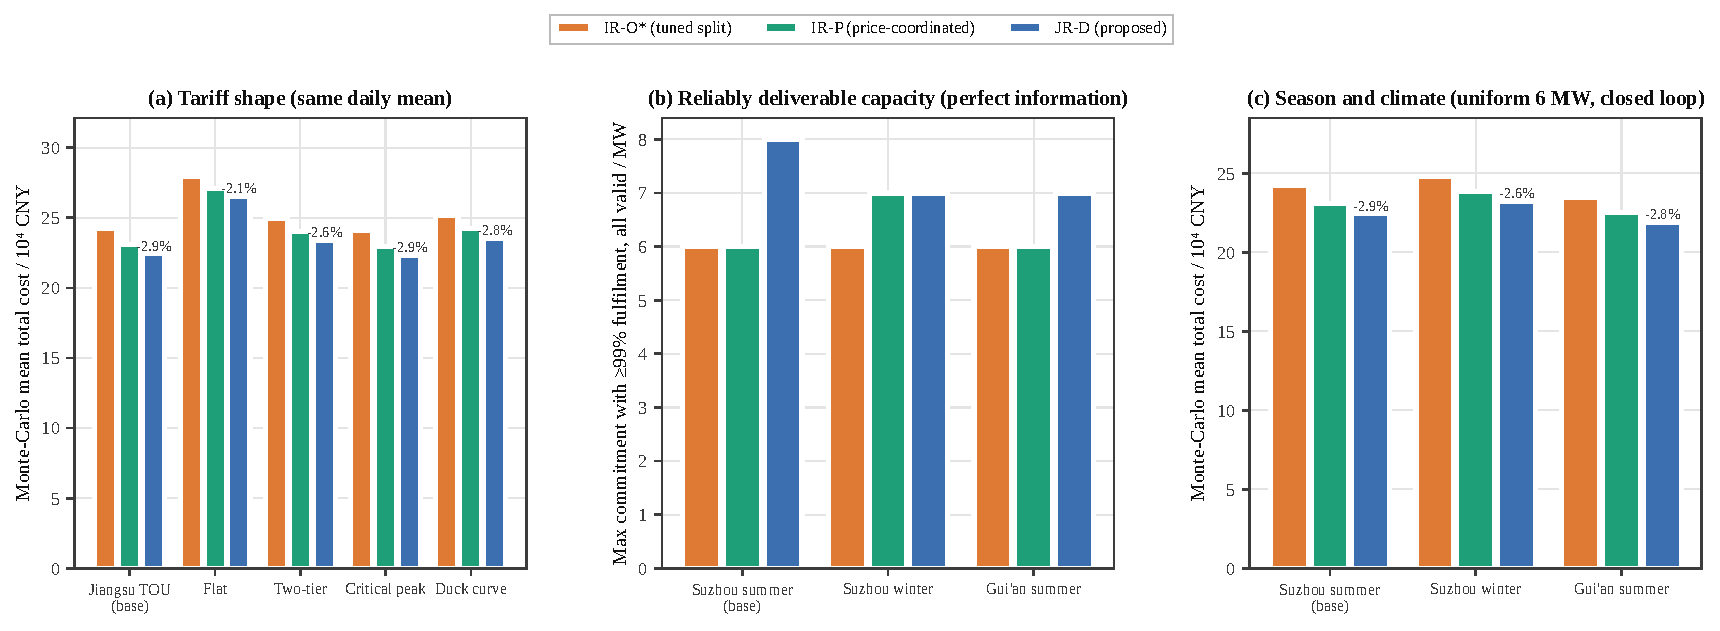
\includegraphics[width=0.98\textwidth]{fig20_generalization.pdf}
\caption{Generalisation. (a) TOU tariff shapes with the same daily mean (labels: JR-D relative to the stronger
benchmark); (b) reliably deliverable capacity under perfect information and (c) closed-loop mean cost for three climates.}
\label{fig:gen}
\end{figure*}

\begin{table}[!t]
\caption{Seasons and climates (same computing traces, Jiangsu rules and tariff).}
\label{tab:climate}
\centering\footnotesize
\setlength{\tabcolsep}{2.4pt}
\begin{tabular}{@{}lcccccc@{}}
\toprule
Case & \makecell{$\Pcap$\\(MW)} & \makecell{Mean\\COP} & \makecell{PV\\(MWh/d)} & \makecell{Reliable cap.\\IR-O*/IR-P/JR\\(MW)} & \makecell{All valid\\IR-O*/IR-P/\\JR-D} & \makecell{JR-D\\vs IR-P}\\
\midrule
\makecell[l]{Suzhou\\summer} & 16.03 & 5.13 & 38.9 & 6 / 6 / \textbf{8} & 90 / 95 / \textbf{100\%} & $-2.86\%$\\
\makecell[l]{Suzhou\\winter} & 15.51 & 7.00 & 26.0 & 6 / 7 / \textbf{7} & 95 / 95 / \textbf{100\%} & $-2.61\%$\\
\makecell[l]{Gui'an\\summer} & 15.67 & 5.77 & 44.9 & 6 / 6 / \textbf{7} & 95 / 95 / \textbf{100\%} & $-2.80\%$\\
\bottomrule
\multicolumn{7}{@{}p{0.97\columnwidth}@{}}{\scriptsize Reliable capacity under perfect information ($\ge$99\% fulfilment, all events valid); closed loop on 20 days at 6~MW, paired $p=4\times10^{-6}$ in all cases.}
\end{tabular}
\end{table}

Three climates use the same computing traces, Jiangsu rules and tariff: summer in Suzhou (base, maximum 38.3~$^\circ$C),
winter in Suzhou (10 January 2025, minimum $-3.0~^\circ$C) and summer in Gui'an (26 July 2024, maximum 31.7~$^\circ$C), a
national computing hub (\tabref{tab:climate}). In all three, JR-D keeps every event valid on every day and costs about
2.6--2.9\% less than IR-P. In winter and in the cooler climate the cooling load is lower and the COP higher, so less
cooling-related electricity can be shifted and the reliable capacity of JR drops to 7~MW; in winter IR-P also reaches
7~MW. The value of joint recovery thus follows the scarcity of the recovery channel, as Theorem~\ref{thm:closed}
predicts, and is largest in the evening peak of hot summer days. The coincidence of the drivers explains why that peak is
tight (\figref{fig:drivers}): in normal operation the storage discharges in the peak-price hours, which lowers the
17:00--22:00 baseline to about 9.6~MW, and PV has vanished while the price is still high, so reductions must rely more
on deferring computing and extra storage discharge, and the subsequent recovery need is larger.

\subsection{Job-level validation and extensions}
\label{sec:res-ext}

\subsubsection{Job-level validation of the fluid workload model}
\label{sec:res-job}

All results so far rely on the fluid model, in which backlog can be worked off on any idle GPU with any parallelism. To
test this assumption, every closed-loop run is replayed by a job-level executor and settled again. Jobs are sampled from
the joint gang-size--run-time distribution of the traces; every 15~min the deviation of each class from its nominal load
in the fluid plan becomes a target number of busy GPUs, and jobs are scheduled by slack (jobs whose slack is shorter than
one step must run) and back-filled towards the class and total targets. Jobs are rigid: they run as whole gangs at
nominal speed and cannot be accelerated. A pause costs a checkpoint before it (base: 1~min, during which the GPUs still
draw power) and a restart after it (base: 5~min of powered, unproductive time), with a minimum pause of 15~min; these
values follow asynchronous and in-memory checkpointing~\cite{wan2025,wang2023gemini,hu2024acme}. Deviations of the busy
GPUs from the fluid plan are converted into IT power, the cooling deviation is taken up by the electric chillers, and the
storage and gas engine follow the fluid plan.

On the PAI case day (\figref{fig:jobsim}(a)), the fluid plan of JR-D schedules large catch-up after each event (about
$+3$~MW of IT power after E1 and $+3$ to $+5$~MW after E3), mainly of long jobs. Rigid jobs cannot do this: 11,543
GPU$\cdot$h of the planned catch-up cannot be executed, the slack of the jobs is exhausted before E3, and E3 achieves
only 3.7~MW (below the validity threshold of 4.8~MW), so that E3 becomes invalid and the cost rises from 22.84 to
$30.98\times10^4$~CNY (+36\%). The other five strategies also lose at least one event at job level. With the rigid-job
bound \eqref{eq:rigid}, the plan of JR-D changes: E1 mainly pauses medium jobs, E2 medium and long jobs, and E3 all long
jobs, whose backlog (about 3,900~GPU$\cdot$h) is carried into the next day and worked off after their nominal ends
(\figref{fig:jobsim}(b)). The planned cost rises to $25.15\times10^4$~CNY (+10\%), because catch-up in the gaps is no
longer available, and the job-level cost is $26.52\times10^4$~CNY (+5.4\%, mostly pause and restart overheads) with all
three events valid, a tracking error of the grid import of 0.22~MW and only 397~GPU$\cdot$h of planned catch-up left
unexecuted.

\begin{table}[!t]
\caption{Job-level execution on 52 operating days.}
\label{tab:jobsim}
\centering\footnotesize
\setlength{\tabcolsep}{2.5pt}
\begin{tabular}{@{}lccc@{}}
\toprule
\makecell[l]{Load $\cdot$ recovery\\model of the plan} & \makecell{All events valid:\\JR-D / best IR} & \makecell{Job-level cost of JR-D\\vs best IR} & \makecell{JR-D job-level\\vs fluid cost}\\
\midrule
PAI $\cdot$ fluid & 5.8\% / 0\% & $-4.7\%$ (IR-P, 52/52) & +34.9\%\\
PAI $\cdot$ rigid & 86.5\% / 46--60\% & $-3.0\%$ (IR-P, 50/52) & +6.9\%\\
Acme $\cdot$ fluid & 65\% / 33--35\% & $-7.8\%$ (IR-P, 50/52) & +30.7\%\\
Acme $\cdot$ rigid & 98\% / 75--87\% & $-5.0\%$ (IR-O*, 51/52) & --\\
\bottomrule
\multicolumn{4}{@{}p{0.97\columnwidth}@{}}{\scriptsize Best IR: IR-O* and IR-P; numbers of days on which JR-D is cheaper in brackets; paired $p\le10^{-9}$.}
\end{tabular}
\end{table}

\begin{figure*}[!t]
\centering
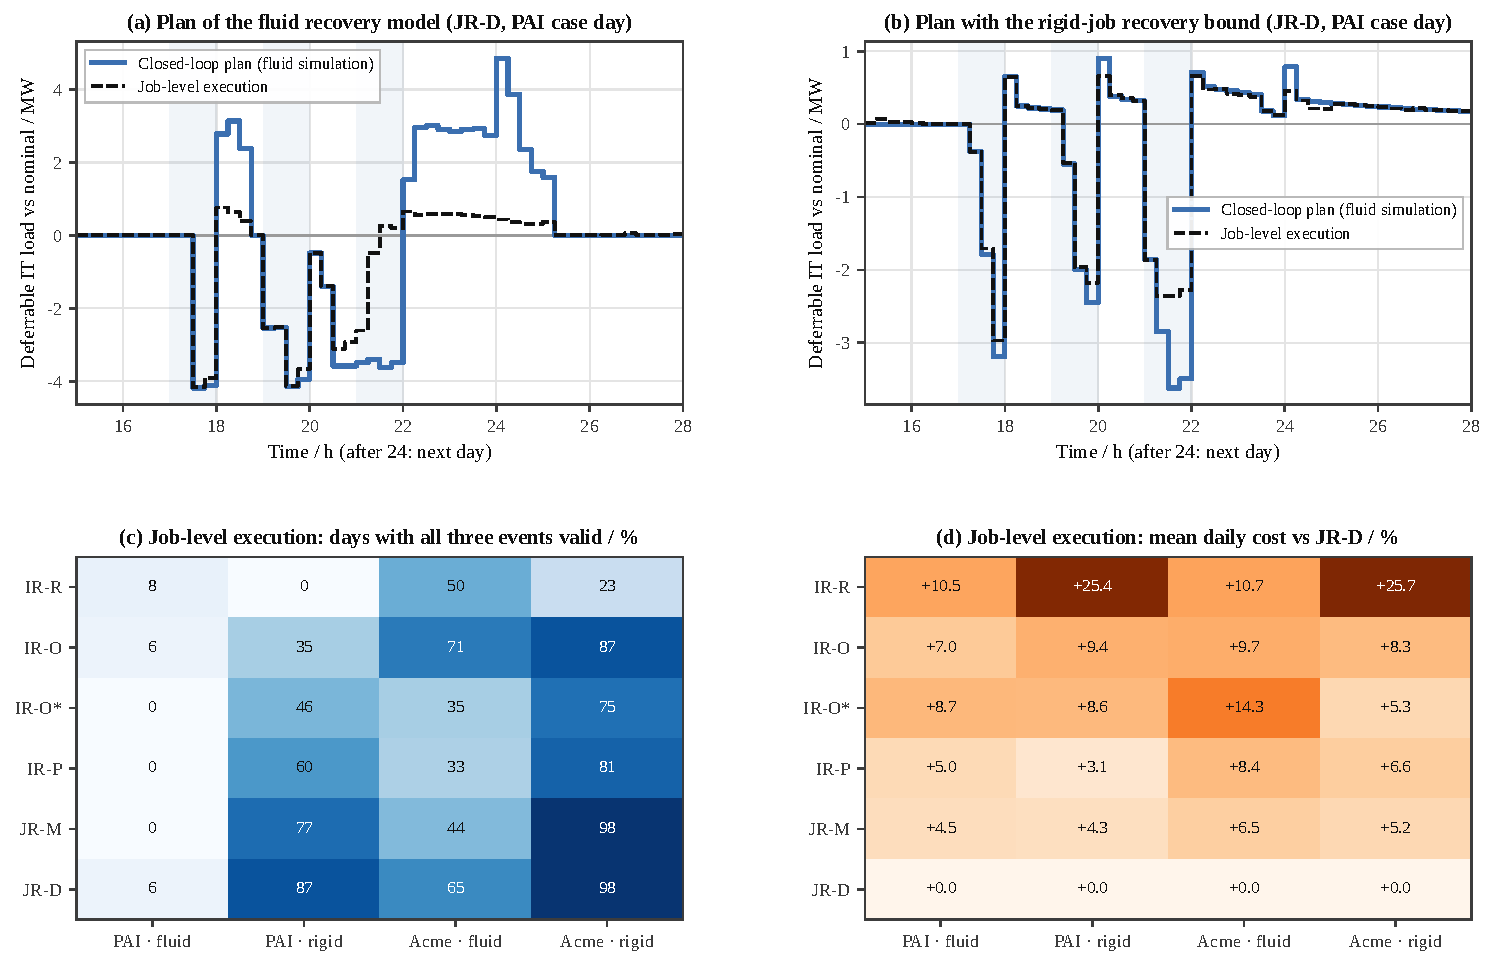
\includegraphics[width=0.90\textwidth]{fig22_jobsim.pdf}
\caption{Job-level validation. (a)(b) Closed-loop plan and job-level execution of JR-D on the PAI case day (deferrable
IT load relative to nominal) with (a) the fluid recovery model and (b) the rigid-job recovery bound; (c)(d) share of the
52 days with all events valid and mean daily cost relative to JR-D at job level.}
\label{fig:jobsim}
\end{figure*}

On the 52 days (\tabref{tab:jobsim}, \figref{fig:jobsim}(c)(d)), the fluid model proves too optimistic for rigid long
jobs: plans made with it fail at job level almost every day with the PAI load (no strategy keeps all events valid on
more than 8\% of the days) and underestimate the cost by 11--38\%; with the Acme load, where long jobs carry 80\% of the
work, all events remain valid on only 33--71\% of the days. The rigid-job bound makes the plans executable: JR-D keeps
all events valid on 98\% of the days with the Acme load and on 86.5\% (instead of 5.8\%) with the PAI load, with a
tracking error of about 0.2--0.3~MW, and the job-level cost of the same strategy is 12--16\% lower when planned with the
rigid model (JR-D: 22.13 against $25.12\times10^4$~CNY per day for Acme, 26.13 against 30.39 for PAI). The advantage of
joint recovery persists at job level: it widens to 4.7--7.8\% with fluid plans and is 5.0\% (Acme) and 3.0\% (PAI) with
rigid plans, not less than the 2.9--3.1\% of the fluid evaluation. The rigid jobs restrict catch-up in the gaps, so more
of the channel can only recharge storage, at efficiency $\eta$; independent recovery relies on catch-up in the gaps to
free the virtual storage and suffers more, whereas joint recovery carries the long-job backlog beyond the last event. In
the rigid variant the fluid accounting by arrival batches reports overdue work that does not exist (46--638
GPU$\cdot$h$\cdot$h for Acme), because the tails of finishing delayed jobs supply catch-up that the first-order bound
$B/\tau_c$ omits; the job-level results, with zero overdue work, are therefore authoritative for this variant. On its
own, the LLM-era Acme load leaves the conclusions of the fluid model unchanged: JR-D is 3.1\% cheaper than IR-P (52/52
days, $p=3.5\times10^{-10}$), similar to the 2.9\% with PAI, with all events valid on 100\% against 98\% of the days.

\begin{figure*}[!t]
\centering
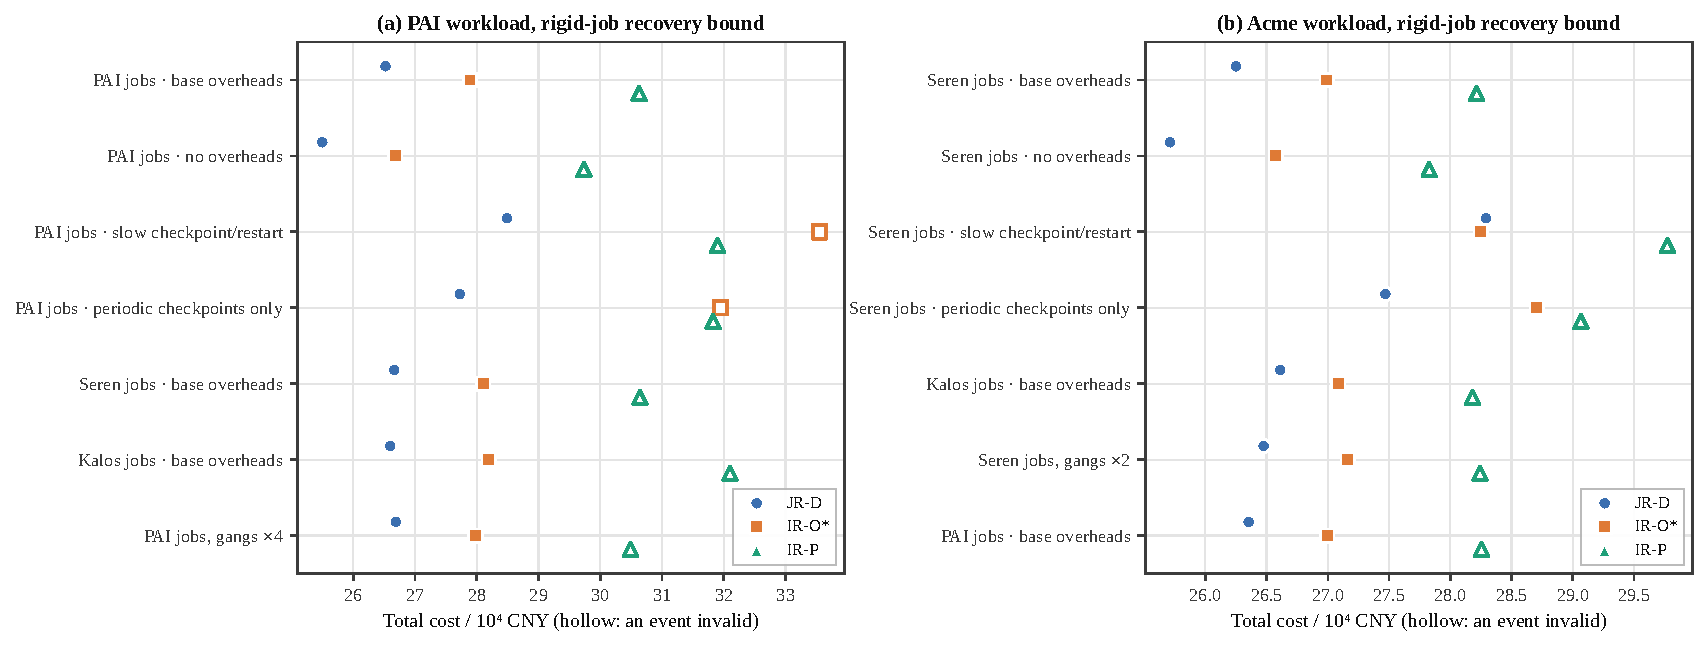
\includegraphics[width=0.90\textwidth]{fig23_jobmix.pdf}
\caption{Job-level total cost on the case day for different job mixes and pause overheads (rigid-job recovery bound;
hollow markers: at least one event invalid).}
\label{fig:jobmix}
\end{figure*}

The job mix and overheads are varied on the case day in \figref{fig:jobmix}: jobs from Seren or Kalos (pre-training
jobs with 512--1,024 GPUs), gang sizes scaled by 2 or 4, and no, base, slow (10-min checkpoint, 15-min restart, 30-min
minimum pause) or periodic-only checkpointing (every 30~min, losing the progress since the last checkpoint). Plans made
with the rigid model are executable in all settings: in all 14 load--job combinations JR-D keeps all three events valid
and is the cheapest in 13; the exception is the Acme load with slow checkpoint and restart, where IR-O* is 0.15\% cheaper
with all events valid as well. With the PAI load the job-level cost exceeds the fluid evaluation by 1.4\% without
overheads, 5.5\% with base overheads and 13\% with slow ones. The strongest benchmarks are more sensitive to overheads:
with the PAI load and slow checkpointing IR-O* keeps only one event valid (two with periodic checkpointing only), and IR-P
loses at least one event in every setting (two with Kalos jobs); with base overheads JR-D is 4.9\% (PAI) and 2.7\%
(Acme) cheaper than IR-O* at job level. With base overheads a day sees 650--4,100 pauses (more with small jobs), about
1,100--1,400~GPU$\cdot$h of restarts and 220--300~GPU$\cdot$h of lost checkpoint progress, together about 1.3--1.6~MWh,
which raises the daily cost of JR-D by 2--4\%; slow checkpointing roughly triples these overheads. Gang granularity
matters little: even when the largest paused job draws 0.7--1.2~MW, the cost of JR-D changes by only 0.3--1.4\%, since
the executor back-fills with small jobs and other classes absorb the granularity error. All pauses at the start of an
event complete within the same minute, so the deferrable IT power steps by about 3--4~MW within 1~min; if the grid
limits ramps, the pauses can be staggered over a few minutes or the IT ramp limit of \secref{sec:computing} can be
imposed. Power swings of synchronous training at the second and iteration scale~\cite{choukse2025} are outside the 15-min
scheduling considered here.

\subsubsection{Pause overheads and multi-level power capping}
\label{sec:ext-overhead}

The fluid model is extended by the pause overhead $o_c$ of \eqref{eq:backlog} (base: 6~min per newly paused GPU for a
1-min asynchronous checkpoint and a 5-min restart; slow: 25~min for synchronous checkpoints and slow restarts of large
models) and by power capping with one level (power $-30\%$, throughput $-12\%$) or three levels ($-15/-30/-45\%$ power
for $-3/-12/-30\%$ throughput), with uniform 6~MW, re-tuned benchmarks and 26 days (\tabref{tab:overhead},
\figref{fig:ext}(a)).

\begin{table*}[!t]
\caption{Pause overheads and multi-level power capping (26 days, uniform 6~MW).}
\label{tab:overhead}
\centering\footnotesize
\setlength{\tabcolsep}{6pt}
\begin{tabular}{@{}lcccc@{}}
\toprule
Setting & \makecell{JR-D cost\\($10^4$~CNY)} & \makecell{JR-D vs\\IR-P} & \makecell{All valid\\JR-D/IR-P/IR-O*} & \makecell{Overhead (GPU$\cdot$h)\\JR-D/IR-P/IR-O*}\\
\midrule
Base (fluid) & 22.50 & $-2.8\%$ (25/26) & 100/96/92\% & --\\
Overhead 6~min & 23.20 & $-2.6\%$ (25/26) & 96/88/62\% & 1,465/1,761/2,919\\
Overhead 25~min & 24.10 & $-2.3\%$ (24/26) & 100/81/27\% & 3,869/4,686/5,624\\
One capping level & 21.87 & $-4.8\%$ (26/26) & 100/62/65\% & --\\
Three capping levels & 21.83 & $-4.5\%$ (26/26) & 100/65/65\% & --\\
Three levels + 6~min & 22.55 & $-2.6\%$ (22/26) & 96/58/38\% & 1,169/1,111/244\\
\bottomrule
\multicolumn{5}{@{}l@{}}{\scriptsize Paired Wilcoxon $p<4\times10^{-4}$ in all settings.}
\end{tabular}
\end{table*}

Pause overheads raise the cost by 3.1\% (6~min) and 7.1\% (25~min), the same order as in the job-level simulation
(2--4\%). JR-D remains the cheapest, with its advantage over IR-P narrowing from 2.8\% to 2.3\%, but the reliability of
the independent benchmarks falls faster: IR-O* keeps all events valid on only 62\% and 27\% of the days. Since the
overhead counts newly paused GPUs, the static split of IR-O*, which pauses and resumes repeatedly between events, incurs
the largest overhead, whereas JR-D defers long jobs continuously and incurs the smallest (half that of IR-O* at 6~min).
Power capping makes every strategy cheaper and widens the advantage of joint recovery: the cost of JR-D falls by 2.8\%
and its advantage over IR-P grows to 4.5--4.8\% (26/26 days). The throughput loss of capping becomes additional
backlog; IR-P keeps all events valid on only 62--65\% of the days instead of 96\%, while JR-D stays at 100\%, consistent
with joint recovery scheduling the backlog left by capping together with the storage deficit across events. Three
levels are only 0.2\% cheaper than one, so a single level of $-30\%$ power for $-12\%$ throughput is nearly sufficient.
With both capping and overheads the two effects largely cancel: JR-D costs $22.55\times10^4$~CNY, close to the base, and
is still 2.6\% cheaper than IR-P (22/26 days); IR-O* then caps more and pauses less (244~GPU$\cdot$h of overhead) but
keeps all events valid on only 38\% of the days.

\subsubsection{Green-power direct supply with offshore wind}
\label{sec:ext-wind}

Offshore wind from the Rudong site is connected behind the meter without grid export under the green-power
direct-connection policy~\cite{ndrc2025green}, which requires the self-consumed share to be at least 60\% of the usable
generation and at least 30\% (35\% before 2030) of the user's consumption. The connection limit stays at 16.0~MW, the
day-ahead wind forecast has an error of 15\% of the capacity (root mean square), and each operating day re-solves the
day-ahead commitment and the IR-P price with its own forecast (\tabref{tab:wind}, \figref{fig:wind}). Without DR, the
renewable share of consumption averages 25.6/40.0/58.4/71.9\% at 5/10/20/40~MW of wind, and the self-consumed share stays
at 100\% up to 10~MW and falls to 89.1\% at 20~MW and 65.5\% at 40~MW. The policy evaluates both shares annually; on
average about 7~MW of wind meets the 30\% share and 40~MW still meets the 60\% self-use, while on a daily basis both
are met on most days at 20~MW (94\%; 91\% with the 35\% threshold), so a wind capacity of about 1.25 times the connection
limit matches the policy best.

\begin{table*}[!t]
\caption{DR with behind-the-meter offshore wind (26 operating days).}
\label{tab:wind}
\centering\footnotesize
\setlength{\tabcolsep}{6pt}
\begin{tabular}{@{}ccccccc@{}}
\toprule
\makecell{Wind\\(MW)} & \makecell{Wind\\(MWh/d)} & \makecell{Commitment sum\\(MW, declared)} & \makecell{JR-D DR revenue\\($10^4$~CNY/d)} & \makecell{JR-D cost\\($10^4$~CNY)} & \makecell{JR-D vs\\IR-P} & \makecell{All valid\\JR-D/IR-P/IR-O*}\\
\midrule
0 & 0 & 17.7 (100\%) & 6.21 & 22.46 & $-2.5\%$ & 100/96/96\%\\
5 & 50 & 13.4 (96\%) & 4.41 & 18.99 & $-6.6\%$ & 92/58/92\%\\
10 & 100 & 7.8 (92\%) & 2.36 & 16.21 & $-6.6\%$ & 77/46/58\%\\
20 & 199 & 6.6 (100\%) & 2.08 & 10.77 & $-5.9\%$ & 85/73/65\%\\
\bottomrule
\multicolumn{7}{@{}l@{}}{\scriptsize Paired differences: 25/26, 24/26, 24/26 and 21/26 days cheaper; $p$ = $9\times10^{-8}$, $1\times10^{-6}$, $3\times10^{-6}$ and 0.002.}
\end{tabular}
\end{table*}

\begin{figure*}[!t]
\centering
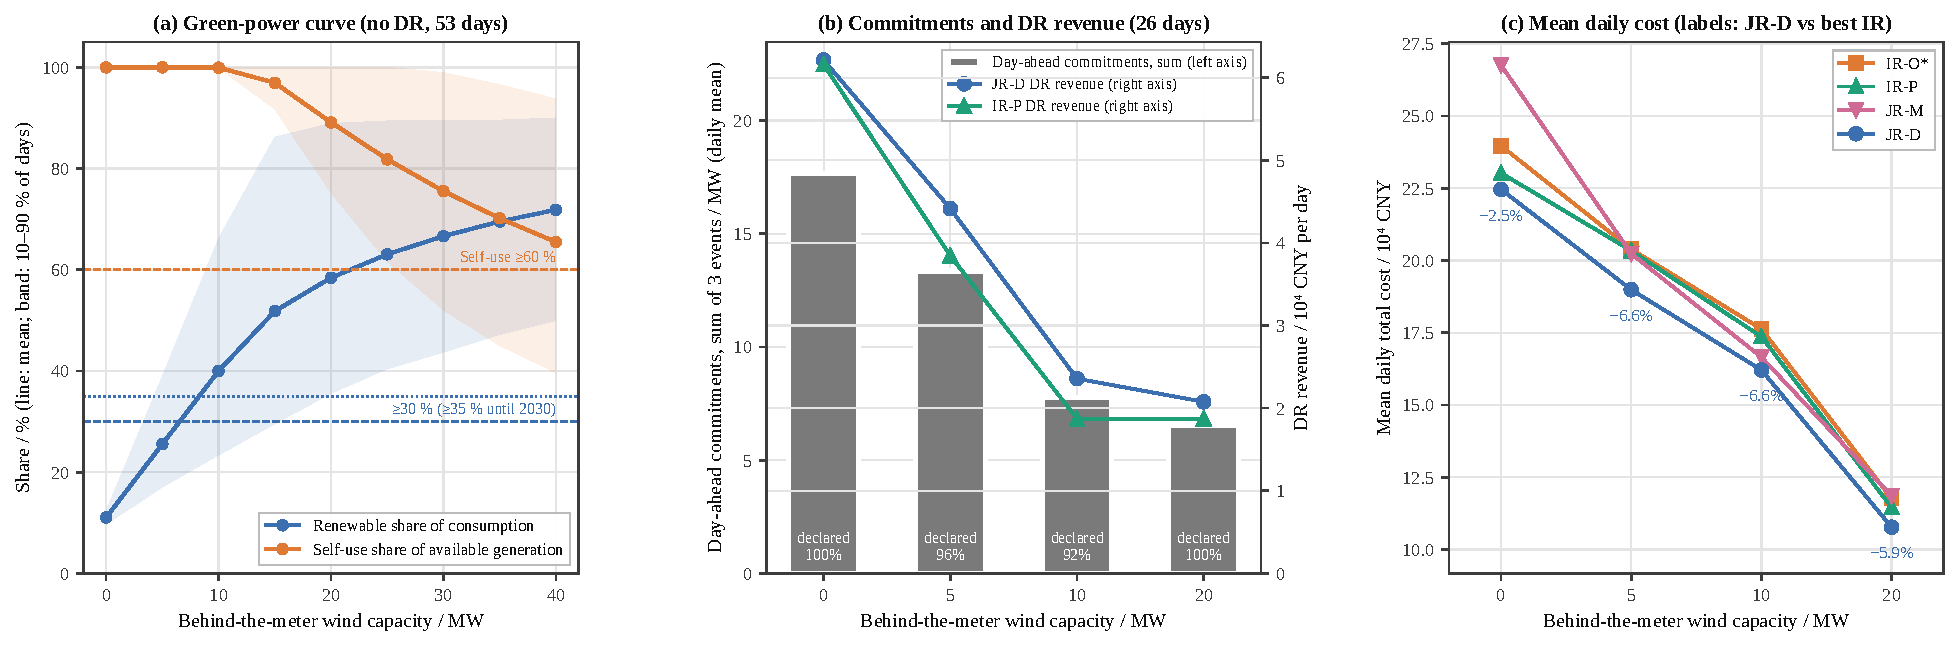
\includegraphics[width=0.98\textwidth]{fig26_wind.pdf}
\caption{Green-power direct supply with offshore wind. (a) Renewable share of consumption and self-used share of the
available generation without DR (lines: means; bands: 10--90\% of the days) with the policy thresholds; (b) sum of the
day-ahead commitments (bars; share of declared events inside) and DR revenue; (c) mean daily cost (labels: JR-D
relative to the strongest independent benchmark).}
\label{fig:wind}
\end{figure*}

The meter-based baseline makes the deliverable commitments fall quickly with the wind capacity. The baseline is taken
from the meter data of the reference days and thus inherits their wind; once the wind of the operating day deviates from
that average, the metered ``reduction'' deviates as well even if the load does not. The total commitment falls from 17.7
to 6.6~MW at 20~MW of wind ($-63\%$), the DR revenue of JR-D drops to one third, and on days with little forecast wind the
day-ahead model declares some events with zero commitment (8\% of the events at 10~MW). The saved electricity cost far
exceeds the lost DR revenue: the daily cost of JR-D falls from 22.5 to $10.8\times10^4$~CNY at 20~MW. The advantage of
joint recovery widens with wind, to 5.9--6.6\% against IR-P (2.5\% without wind), because forecast errors shift the net
load during the events and reduce validity for all strategies, but less for joint recovery, which keeps more margin for
corrections by planning backlog and storage across events (all events valid on 77--92\% of the days against 46--73\%
for IR-P). The differences come from days with weak and mispredicted wind, whereas on the windy case day (122 and
244~MWh at 10 and 20~MW) commitments are small and easy to meet and the strategies differ by less than 1\%. Measuring
the baseline at the grid meter thus counts the fluctuations of behind-the-meter wind as response or counter-response
(see~\cite{chao2011} for baseline choice in general); metering the wind separately and settling on the load net of wind
would preserve the flexibility of the data center, which needs clarification at the policy level.

\subsubsection{Winter waste-heat recovery}
\label{sec:ext-heat}

In winter, a water-source heat pump (3~MW$_{\mathrm{el}}$, COP 3.5) lifts the waste heat of the chilled-water return to
a nearby heat network through a hot-water tank \eqref{eq:heat}, with the gas boiler as backup. The case day is the cold
day of 10 January 2025 (daily mean 0.4~$^\circ$C), the heat demand is about 5.3~MW$_{\mathrm{th}}$ (127~MWh$_{\mathrm{th}}$
per day), the connection limit stays at the 15.5~MW without heating, and the 26 coldest winter days are the operating
days (\tabref{tab:heat}, \figref{fig:heat}).

\begin{table*}[!t]
\caption{Winter waste-heat recovery (26 coldest days, uniform 6~MW).}
\label{tab:heat}
\centering\footnotesize
\setlength{\tabcolsep}{6pt}
\begin{tabular}{@{}lccccc@{}}
\toprule
Setting & \makecell{JR-D cost\\($10^4$~CNY)} & \makecell{JR-D vs\\IR-P} & \makecell{All valid\\JR-D/IR-P/IR-O*} & \makecell{Waste-heat share\\JR-D / IR-P} & \makecell{Boiler (MWh)\\JR-D / IR-P}\\
\midrule
Gas boiler only & 28.25 & $-2.1\%$ (25/26) & 100/96/96\% & 0 / 0 & 138.6 / 138.6\\
Heat pump, no tank & 23.56 & $-4.4\%$ (26/26) & 100/69/96\% & 82.6 / 77.4\% & 24.1 / 31.3\\
Heat pump + 20~MWh & 23.56 & $-2.3\%$ (25/26) & 100/96/96\% & 97.1 / 91.4\% & 4.1 / 12.1\\
Heat pump + 40~MWh & 23.88 & $-1.4\%$ (25/26) & 100/96/92\% & 99.9 / 99.4\% & 0.2 / 0.8\\
\bottomrule
\multicolumn{6}{@{}l@{}}{\scriptsize Boiler heat includes the first 6~h of the next day; paired Wilcoxon $p<10^{-5}$.}
\end{tabular}
\end{table*}

\begin{figure*}[!t]
\centering
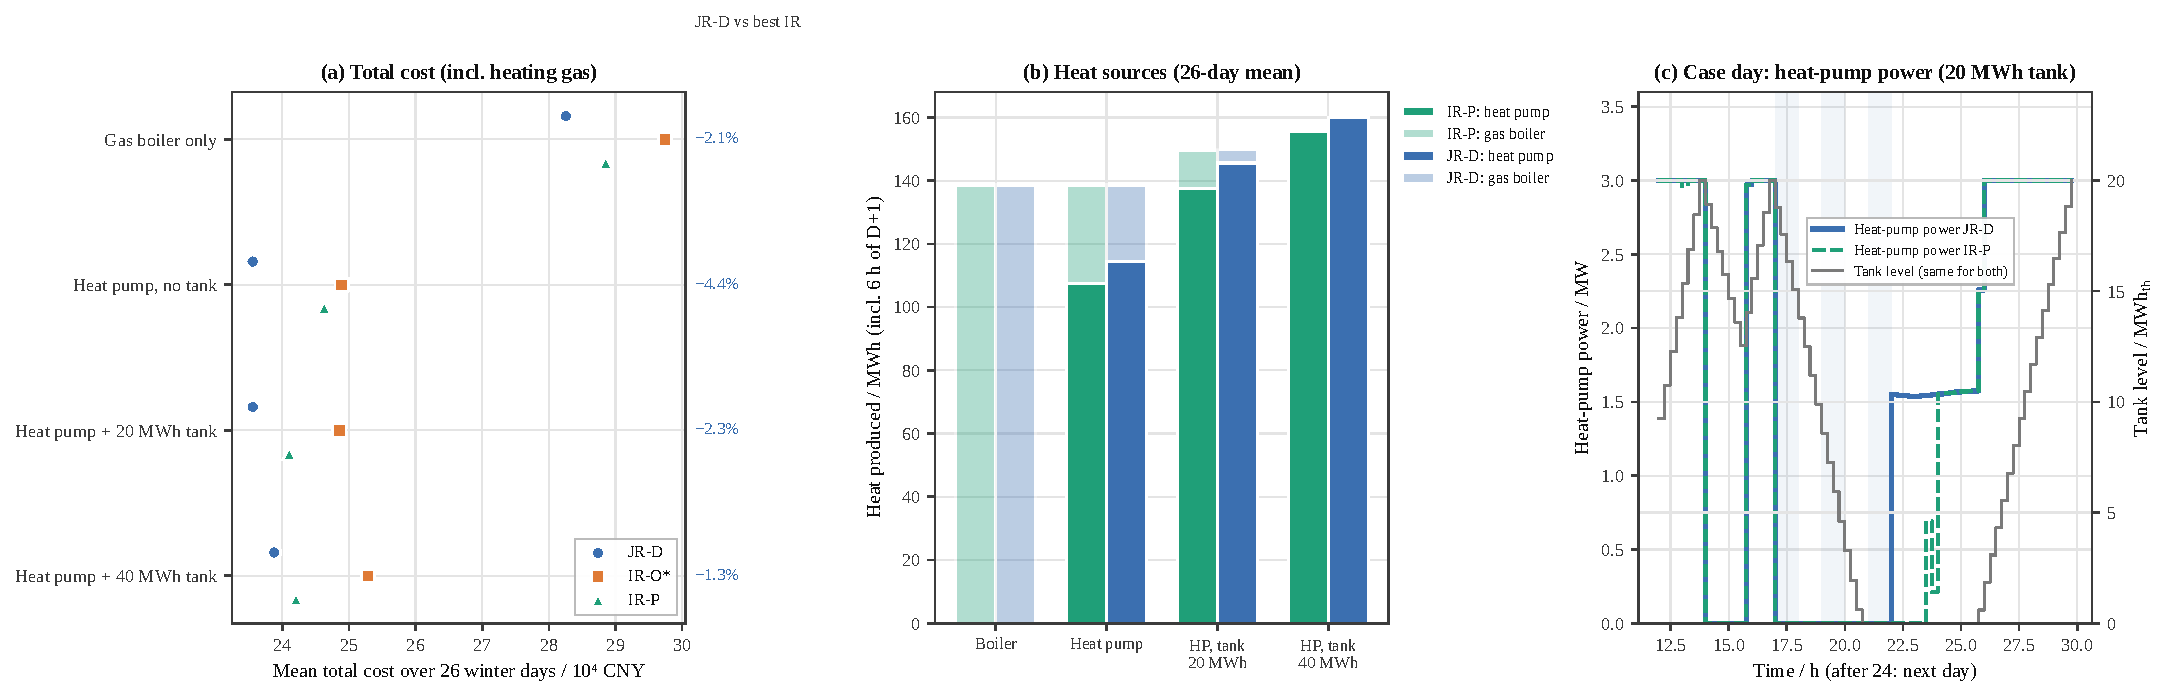
\includegraphics[width=0.98\textwidth]{fig27_heat.pdf}
\caption{Winter waste-heat recovery. (a) Mean total cost on the 26 coldest days including heating gas (right: JR-D
relative to the strongest independent benchmark); (b) heat produced by the heat pump and the gas boiler; (c) heat-pump
power and tank level on the case day with the 20-MWh tank.}
\label{fig:heat}
\end{figure*}

Waste-heat recovery pays off by itself: it lowers the daily cost by 15.5--16.6\% against boiler heating (4.4--4.7$\times
10^4$~CNY per day for JR-D) and the emissions by 16--19~t of CO$_2$ per day. Without a tank, the heat pump competes with
catch-up computing for the channel: its load is part of the baseline, so switching it off during an event counts as
reduction, but the heat demand continues and the heat pump must catch up afterwards, exactly when catch-up computing and
battery recharging need the headroom. The IT side of independent recovery takes this headroom first, so IR-P keeps all
events valid on only 69\% instead of 96\% of the days and burns more boiler gas, while joint recovery, which schedules
the heat pump together with the other states, widens its advantage to 4.4\% (26/26 days). A tank decouples heating from
the events: the heat pump stops during the events, the tank supplies the heat and is recharged afterwards. All strategies
then keep the events valid on 96--100\% of the days and the advantage returns to 2.3\%, but joint recovery recovers about
6 points more waste heat (boiler heat 4.1 against 12.1~MWh), because after E3 it gives the headroom to the heat pump
first whereas independent recovery gives it to catch-up computing (\figref{fig:heat}(c): JR-D restarts the heat pump right
after E3, IR-P about 1.5~h later, with the boiler covering the gap). A larger tank is not always better: the 40-MWh tank
already shifts all peak-period heat-pump load to the valley hours in normal operation, which lowers the baseline in the
event hours by about 0.7~MW against no tank and 0.3~MW against the 20-MWh tank (the same mechanism as for large
batteries in \secref{sec:res-capacity}); JR-D then costs 1.4\% more than with the 20-MWh tank and its advantage shrinks to
1.4\%.

\subsection{Discussion}
\label{sec:discussion}

The results support three practical implications. First, consecutive DR should be bid and settled as a whole: the
capability region of joint recovery is described by the stand-alone capabilities and one cross-event energy budget, and
declaring these virtual-battery parameters instead of one value per event lets the grid operator call more capacity with
the same reliability. Second, the main value of joint recovery lies in the reliably deliverable capacity rather than in
the operating cost at moderate commitments, and it is largest when the recovery channel is scarce: hot evening peaks,
short gaps, tight connection margins, liquid cooling, smaller batteries or a heat pump without a tank. Third, joint
recovery can be implemented without merging the IT and facility control systems, through a few plan--price exchanges per
15~min, whereas a one-shot price signal is insufficient. The settlement rules matter as well: the rebound charge, the
baseline method with storage arbitrage and behind-the-meter wind, and ramp requirements change what the data center
can deliver and should be designed together with its flexibility.

The study has limitations. The fluid workload model is optimistic for rigid gang-scheduled jobs; the rigid-job bound is
a first-order approximation, and the job-level executor is a slack-based heuristic without job dependencies, network
topology or communication overheads. The PAI trace predates LLMs and the Acme trace stems from one institution, while
frontier pre-training jobs may use thousands of GPUs. Only the call of the last event is uncertain, the scenario sets are
small and deterministic, and the ambiguity set covers only the scenario probabilities (a Wasserstein
ball~\cite{esfahani2018} would also cover unseen outcomes). The capability region is computed under perfect information.
The distributed scheme approximates the proximal term by tangent cuts and does not model communication delays, losses,
asynchronous updates or strategic behaviour. Thermal inertia, policy and waste-heat parameters take typical values, the
wind forecast errors are synthetic, the season and climate tests replace only the weather, and the system is aggregated
on one bus without distribution network constraints.


\section{Conclusions}
\label{sec:conclusion}

As AI computing drives a rapid growth of data center electricity demand, AI data centers are increasingly expected to
respond to several DR events within one evening peak. This paper proposed a coordinated scheduling method for
consecutive DR in AI data center integrated energy systems that jointly recovers the computing backlog and the storage
across events, from the day-ahead commitment to intraday operation. Through theoretical analysis and case studies on a
16,000-GPU data center with 52 out-of-sample operating days, the main conclusions are summarised as follows.
\begin{enumerate}[label=(\arabic*),leftmargin=1.9em,itemsep=1.5pt]
\item Consecutive events leave a two-sided debt, deferred computing and depleted storage, that competes for one
connection-limited recovery channel. Independent recovery must repay the whole debt and retains only 38--39\% of the
next event's stand-alone capability for gaps of up to 1~h, whereas joint recovery repays only what the next event needs
and restores 96\% within 0.75~h from the same post-event state. The lag-bounded backlog constraint is exact
(Lemma~\ref{lem:edf}); the capability bound held in all 80 cases, the closed form of the recovery value matched the LP
within $10^{-5}$~MW, and the single channel price was confirmed with KKT residuals of $2\times10^{-12}$.
\item The main value of joint recovery is the reliably deliverable capacity. It raises the capacity that is delivered on
at least 95\% of the days from 6 to 8~MW per event (+33\%), which is equivalent to about 9--12~MWh of battery or 2.9~MW
of connection capacity, while price-coordinated independent recovery reaches this reliability at no commitment level.
The capability region of joint recovery is the single-event box intersected with one cross-event energy budget and can
be declared by four numbers; independent recovery shrinks this budget by 18\% even with a hindsight-optimal split, and a
one-shot price delivers only 60\% of the uniform capability on average because the IT side's response is not unique.
\item In closed-loop operation, joint recovery keeps all three events valid on all 52 days (benchmarks: 86--98\% of the
days) and lowers the total cost by 2.9--4.0\% against the strongest benchmark of each setting ($p<10^{-9}$), and by
14--16\% when the commitments approach the single-event capabilities; coupled commitment with joint recovery is 12.6\%
cheaper than single-event assessment with independent recovery. The saving comes from the rebound charge (78\%) when
rebound is priced and from the additional DR payment (86\%) under the Jiangsu settlement alone, not from energy
arbitrage.
\item Joint recovery can be distributed: when the IT scheduler and the facility controller exchange only power plans
and prices, 1, 3 and 10 exchanges per 15-min step recover 67\%, 85\% and 97\% of its advantage over the strongest
independent benchmark, and the converged price equals the recovery-channel price. Distributionally robust commitments
lower both the mean (by up to 0.26\%) and the worst-decile cost (by up to 0.4\%) out of sample, the scenario MPC adds
only an insignificant 0.4\% when the last event is uncertain, and the advantage of joint recovery holds across tariff
shapes ($-2.1$ to $-2.9\%$), seasons and climates ($-2.6$ to $-2.9\%$), liquid cooling ($-7.4\%$), thermal inertia
($-2.2\%$) and power capping, whereas tight IT ramp limits compress it (0.8\% at 1~MW per 15~min).
\item The fluid workload model is too optimistic for rigid gang-scheduled training: plans made with it fail at job level
on most days. With the rigid-job recovery bound the plans become executable (all events valid on 98\% and 86.5\% of the
days for the Acme and PAI loads), and joint recovery stays 3.0--5.0\% cheaper than the strongest benchmark at job level.
With behind-the-meter offshore wind the meter-based baseline reduces the deliverable commitments by 63\% at 20~MW, while
the advantage of joint recovery widens to 5.9--6.6\%; winter waste-heat recovery saves about 16\% of the daily cost
against boiler heating, and a hot-water tank turns the heat pump into a flexible load that is recharged after the events.
\end{enumerate}

Future work will extend the capability region to forecast errors and to the clearing of virtual-battery bids in DR
markets, schedule rigid jobs directly in the planning model and replace the first-order recovery bound by kernels based
on remaining run times, adopt Wasserstein ambiguity sets, and study the distributed coordination under communication
delays, asynchronous updates and strategic behaviour, as well as uncertainty in event timing and duration and
multi-site data center clusters with network constraints.

\section*{CRediT authorship contribution statement}
\textbf{First Author:} Conceptualization, Methodology, Software, Writing -- original draft.
\textbf{Second Author:} Data curation, Validation, Visualization.
\textbf{Third Author:} Formal analysis, Writing -- review \& editing.
\textbf{Corresponding Author:} Supervision, Funding acquisition, Writing -- review \& editing.
[Names and roles to be completed by the authors.]

\section*{Declaration of competing interest}
The authors declare that they have no known competing financial interests or personal relationships that could have
appeared to influence the work reported in this paper.

\section*{Acknowledgements}
[Funding information to be added by the authors.]


\appendix
\titleformat{\section}{\normalfont\normalsize\bfseries\raggedright}{Appendix \thesection.}{0.5em}{}
\section{Supplementary data and parameters}
\label{app:data}
\appendixnumbering

This appendix lists the parameters with their sources, compares the two workload traces and shows the case-day time
series and the coincidence of the drivers. Parameters are tagged as taken from a cited source [S], derived from public
data [D] or assumed [A]; every assumed value is varied in the sensitivity studies of \secref{sec:res-sens}.

\begin{table}[!htb]
\caption{Workload traces: PAI (2020) and Acme Seren (2023).}
\label{tab:acme}
\centering\footnotesize
\setlength{\tabcolsep}{3pt}
\begin{tabular}{@{}lcc@{}}
\toprule
 & PAI 2020 & Acme Seren 2023\\
\midrule
GPU$\cdot$h share of C1/C2/C3 & 6.6 / 43.9 / 49.5\% & 5.3 / 14.2 / 80.5\%\\
Gang size of C3 (GPU$\cdot$h weighted) & 35 & 407\\
Mean run time $\tau_c$ (h) & 0.26 / 3.6 / 26.3 & 0.11 / 4.2 / 39.5\\
Load 17--22~h / daily mean & 1.03 & 1.006\\
Coefficient of variation of daily load & 0.11 & 0.22\\
\bottomrule
\multicolumn{3}{@{}p{0.97\columnwidth}@{}}{\scriptsize Acme C3 gang size: median 256, maximum 1,024 GPUs. The Acme case day is 23 May 2023 (0.99 of the workday mean); its 20 previous workdays form the scenario pool and the later workdays, crossed with hot days and Azure days, the 52 operating days.}
\end{tabular}
\end{table}

\begin{figure}[!htb]
\centering
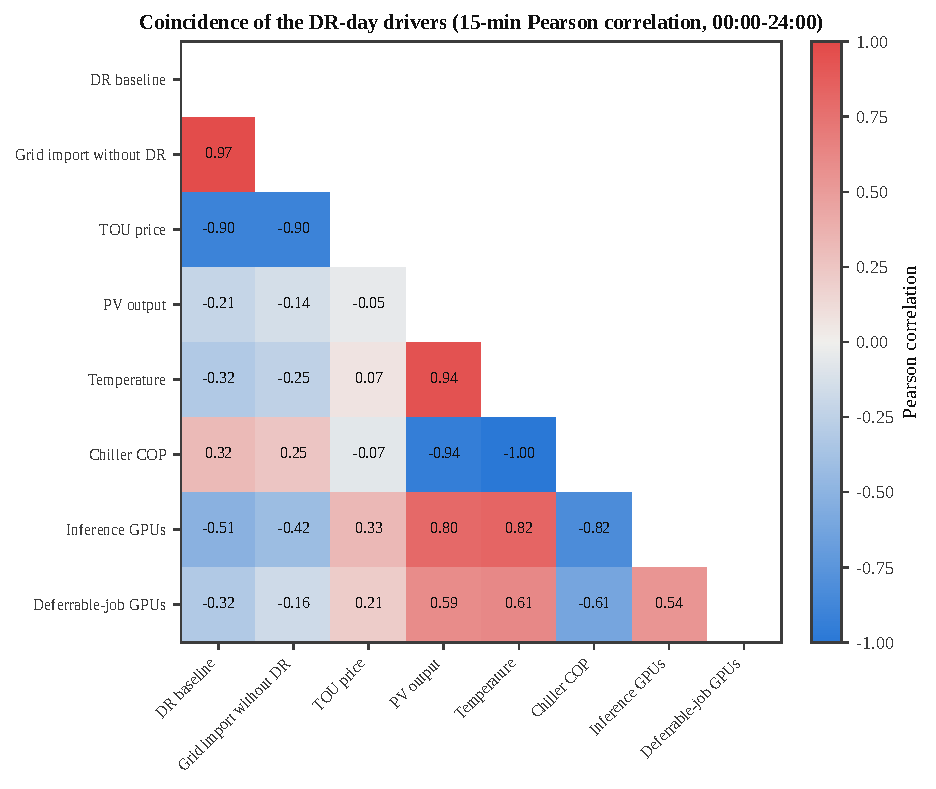
\includegraphics[width=\columnwidth]{fig17_drivers_correlation.pdf}
\caption{Pearson correlation of the DR-day drivers (15-min values). Inference load, temperature and PV peak together in
the afternoon ($r\approx0.8$); the baseline is strongly anti-correlated with the TOU price ($r=-0.90$) because the
storage discharges in the peak-price hours in normal operation.}
\label{fig:drivers}
\end{figure}

\begin{table*}[!t]
\caption{Equipment and energy-system parameters.}
\label{tab:A-equipment}
\centering\footnotesize
\begin{tabularx}{\textwidth}{@{}>{\raggedright\arraybackslash}p{0.25\textwidth}X>{\raggedright\arraybackslash}p{0.17\textwidth}@{}}
\toprule
Parameter & Value & Tag / source\\
\midrule
GPUs, node power, idle share & 16,000 H100-class GPUs; 8.4~kW per 8-GPU node (measured maximum); idle 25\% & [A] / [S]~\cite{latif2024} / [A]\\
Other IT power, auxiliary loads & 0.6~MW storage and network; $a^{\mathrm{aux}}=0.05$; 0.3~MW lighting and offices & [A]\\
Heat and cooling & $\theta=1$~MW$_{\mathrm{th}}$/MW; envelope load 0.3~MW$_{\mathrm{th}}$; chillers 30~MW$_{\mathrm{th}}$ & [A]\\
Chiller COP & $6.0-0.12(T-25)$ limited to 3--7; 4.41--5.61 on the DR day; liquid cooling $15-0.25(T-25)$ & [A]\\
BESS & 6~MW / 12~MWh, SOC 10--95\%, initial 50\%, $\eta_{\mathrm c}=\eta_{\mathrm d}=0.95$, degradation 60~CNY/MWh & [A], cost after~\cite{xu2018}\\
TES (chilled water) & 10~MWh$_{\mathrm{th}}$ (minimum 1), 4~MW$_{\mathrm{th}}$, $\eta=0.98$, loss 0.5\%/h & [A]\\
Gas engine and absorption chiller & 3~MW, $\eta_{\mathrm e}=0.38$, $\eta_{\mathrm h}=0.45$, ramp 1.5~MW/15~min; COP 0.75, 2.7~MW$_{\mathrm{th}}$ & [A]\\
PV & 8~MWp; PVWatts v5: temperature coefficient $-0.37\%$/$^\circ$C, system losses 14\% & [S]~\cite{dobos2014}\\
Connection limit & $\gamma=1.10$ of the typical-day peak $\Rightarrow16.03$~MW (sensitivity 1.0--1.3); minimum import 1.5~MW & [A]\\
Thermal inertia (optional) & 2~MWh$_{\mathrm{th}}$/K; $+3$~K rise and $-2$~K pre-cooling allowed & [A], ASHRAE A1~\cite{ashrae2021}\\
Waste-heat recovery (optional) & Heat pump 3~MW$_{\mathrm{el}}$, COP 3.5 (30 to 65~$^\circ$C); tank 0/20/40~MWh$_{\mathrm{th}}$, loss 0.5\%/h; boiler efficiency 0.9; demand $0.3\max(18-T,0)$~MW$_{\mathrm{th}}$ & [A] / [S]~\cite{meta2018odense}\\
Offshore wind (optional) & 0--40~MW; IEA 15-MW turbine (cut-in 3, rated 10.59, cut-out 25~m/s); farm efficiency 0.9; forecast error 15\% RMS, lag-1 correlation 0.97 & [S]~\cite{gaertner2020} / [A]\\
\bottomrule
\end{tabularx}
\end{table*}

\begin{table*}[!t]
\caption{Computing, market and policy parameters.}
\label{tab:A-market}
\centering\footnotesize
\begin{tabularx}{\textwidth}{@{}>{\raggedright\arraybackslash}p{0.25\textwidth}X>{\raggedright\arraybackslash}p{0.17\textwidth}@{}}
\toprule
Parameter & Value & Tag / source\\
\midrule
Workload composition & Inference $\approx$25\% of the GPUs (Azure shape), training/batch $\approx$40\% (PAI shape), of which 75\% deferrable (C1/C2/C3) & [A] / [D]\\
Inference dynamic-power factor & 0.65 & [A], after~\cite{patel2024}\\
Lag bounds & 0.5 / 1.5 / 3~h (Flex 1--3) & [A], after~\cite{colangelo2025}\\
Delay cost, overdue penalty & 0.5 and 1000~CNY per GPU$\cdot$h and hour & [A]\\
Terminal values & Backlog 0.67~CNY/GPU$\cdot$h; BESS 500~CNY/MWh; TES 100~CNY/MWh$_{\mathrm{th}}$ & computed\\
GPU power capping (optional) & One level $(0.30,0.12)$; three levels $(0.15,0.03)$, $(0.30,0.12)$, $(0.45,0.30)$; events only & [A], after~\cite{acun2026,patel2024}\\
Pause overhead (optional) & $o_c$ = 6~min (1-min checkpoint + 5-min restart) or 25~min & [A], after~\cite{wan2025,wang2023gemini}\\
TOU tariff & Jiangsu 2025 summer: peak 14--22~h ($\times$1.8), valley 0--6 and 11--13~h ($\times$0.35) & [S]\\
DR payment & 3~CNY/kWh (day-ahead), 4.2 (E3, 3~h notice), 4.8 (E3 uncertain, 1~h notice); 1--3 in sensitivity & [S]~\cite{jiangsu2024dr}\\
Validity and payment cap & Mean reduction $\ge$80\% of the commitment (+0.1~MW planning margin); payment $\le$120\% & [S]~\cite{jiangsu2024dr}\\
Shortfall coefficient & $\kappa=1$ (0.5--2) & [A]\\
Rebound charge & 0 and 3~CNY/kW per event (0--6), 2-h window & [A] (policy parameter)\\
Gas price & 3.6~CNY/Nm$^3$, lower heating value 9.89~kWh/Nm$^3$ & [A]\\
Day-ahead risk settings & SP; $\ell_1$ DRO $\delta$ = 0.1/0.2/0.4/0.8/1.2; RO ($\delta=2$); CVaR$_{0.8}$; mean--CVaR$_{0.9}$ ($w=0.5$); 10 scenarios & --\\
PUE cap (optional) & 1.30 / 1.25 / 1.20 & [S]~\cite{ndrc2024dc}\\
Green share (optional) & 60 / 80 / 90\%; green premium 30~CNY/MWh & [S]~\cite{ndrc2024dc} / [A]\\
Emission factors & Grid 0.5617~tCO$_2$/MWh; natural gas 56.1~t/TJ & [S]~\cite{mee2024ef} / IPCC 2006\\
Split of IR-R / IR-O; tuned split & $\alpha=0.41$; $\alpha^*$ back-tested over 0.2--1.0 & computed\\
\bottomrule
\end{tabularx}
\end{table*}



\begin{figure*}[!t]
\centering
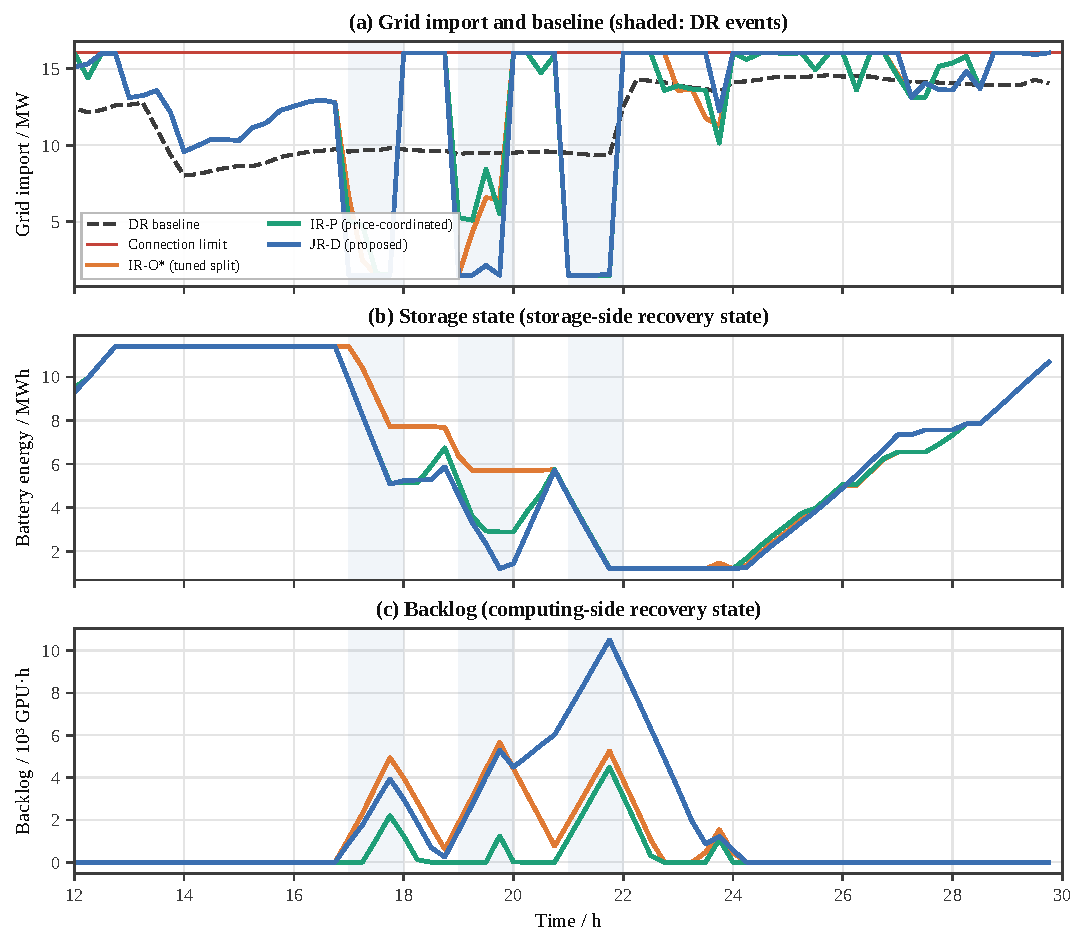
\includegraphics[width=0.82\textwidth]{fig03_timeseries_DAcommit_crb0.pdf}
\caption{Case-day time series (rule setting, coupled commitment): (a) grid import and baseline, (b) BESS energy and
(c) total backlog of JR-D, IR-O* and IR-P.}
\label{fig:ts}
\end{figure*}

\begin{figure*}[!t]
\centering
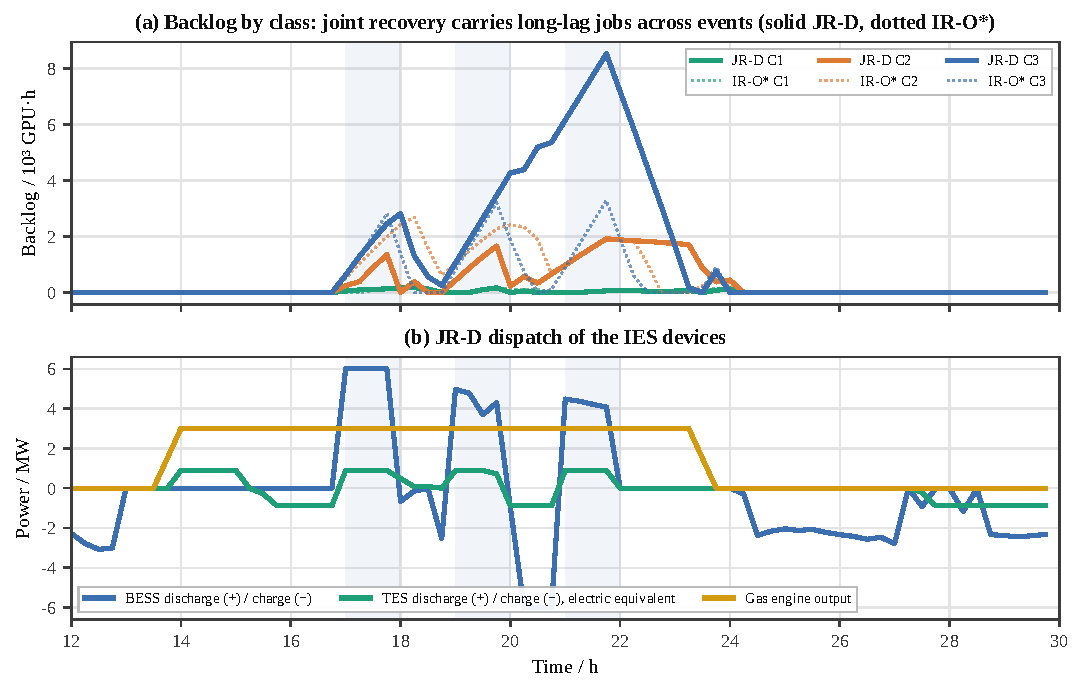
\includegraphics[width=0.82\textwidth]{fig04_backlog_ies_DAcommit_crb0.pdf}
\caption{Case-day backlog by class (solid: JR-D, dotted: IR-O*) and IES dispatch of JR-D (rule setting, coupled
commitment). Joint recovery carries the long-lag class C3 across the events.}
\label{fig:tsbacklog}
\end{figure*}

\section{Proofs and numerical checks}
\label{app:proofs}
\appendixnumbering

\paragraph{Notation and assumptions} For a gap $\Iset=(e_A,s_B)$ of length $\tau$ before event B with duration
$D_B$, let $\eta=\eta_{\mathrm c}\eta_{\mathrm d}$ be the round-trip efficiency (for the TES $\eta^{\mathrm{TC}}\eta^{\mathrm{TD}}$).
Propositions~\ref{prop:bound} and Theorem~\ref{thm:closed} use two assumptions. (H1) Unbiased baseline: without
response the import equals the baseline and the storage is idle in the gap and in event B. (H2) $\varepsilon_t$ and
$\COP_t$ are constant on $\Iset\cup\Tset_B$; otherwise all bounds hold with the largest $\varepsilon$ on that interval
and become slightly looser. Proposition~\ref{prop:region} does not need H1. Under H1, \eqref{eq:cool}--\eqref{eq:elec}
give the deviation of any schedule from the baseline as
\begin{equation}
\Pg_t-\Pb_t=\varepsilon\sum_c\Big(y_{c,t}-\frac{a_{c,t}}{\dt}\Big)+\Pch_t-\Pdis_t+\frac{\Qtc_t-\Qtd_t}{\COP}-\Delta g_t ,
\label{eq:deviation}
\end{equation}
where $\Delta g_t\in[0,g]$ is the additional gas-engine output including its absorption cooling.

\paragraph{Proof of Lemma~\ref{lem:edf}} For one class, let $x_t=y_t\dt$, $A_t=\sum_{s\le t}a_s$, $X_t=\sum_{s\le
t}x_s$, $B_t=A_t-X_t\ge0$, and let $D_t=\sum_{\tau\le t-L/\dt}a_\tau$ be the work due by step $t$, so that
$\Bbar_t=A_t-D_t$. (i)$\Rightarrow$(iii): all work due by $t$ (amount $D_t$) has been executed by $t$, hence $X_t\ge D_t$,
\ie\ $B_t\le\Bbar_t$. (iii)$\Rightarrow$(ii): EDF serves the batches in the order of arrival, so the first $D_t$ units of
execution fall on the batches due by $t$, and $X_t\ge D_t$ completes them in time; since $B_t\ge0$, EDF never executes
work that has not arrived. (ii)$\Rightarrow$(i) is immediate. With several classes sharing the GPUs the argument holds
class by class, because the capacity \eqref{eq:gpucap} only limits $\sum_cy_{c,t}$. A constant limit $\bar Q$ admits
overdue work whenever $\bar Q>\Bbar_t$ and excludes feasible deferrals whenever $\bar Q<\Bbar_t$. $\square$

\paragraph{Proof of Proposition~\ref{prop:bound}} (i) Restricting any feasible schedule of the two-event problem to event
B gives a feasible schedule of the problem with event B alone and the same initial state, hence $\Gamma_B\le\Gamma_B^0$.
(ii) Summing \eqref{eq:deviation} over $\Tset_B$ and using the backlog equation \eqref{eq:backlog},
\begin{multline*}
\Gamma_BD_B=\varepsilon\sum_c\big[B_c(e_B)-B_c(s_B^-)\big]\\
+\sum_{t\in\Tset_{B}}\Big(\Pdis_t-\Pch_t+\frac{\Qtd_t-\Qtc_t}{\COP}\Big)\dt+\sum_{t\in\Tset_{B}}\Delta g_t\dt .
\end{multline*}
By \eqref{eq:lag} the first term is at most $\bar X_B-X(s_B^-)$, the second at most the dischargeable energy $E_s(s_B^-)$,
and the third at most $gD_B$. In the gap, let $C_{\Iset}=\varepsilon\sum_{t\in\Iset}\sum_c(y_{c,t}\dt-a_{c,t})$ be the net
catch-up and $D_{\Iset}$ the net storage intake. Summing \eqref{eq:deviation} over $\Iset$ with $\Pg_t\le\Pcap$ gives the
channel constraint $C_{\Iset}+D_{\Iset}\le H$. Moreover $X(s_B^-)=X_A-C_{\Iset}\ge0$ and $E_s(s_B^-)\le E_s+\phi(D_{\Iset})$ with
$\phi(x)=\eta x$ for $x\ge0$ and $\phi(x)=x$ for $x<0$. Hence
$\Gamma_BD_B-gD_B\le\bar X_B-X_A+E_s+\max\{C+\phi(D):C+D\le H,\ C\le X_A\}$. Catch-up has marginal value one and
recharging $\eta<1$ (discharging in the gap has value one but costs the same amount of catch-up), so the maximum is
attained by catching up first, $C^*=\min(H,X_A)$, and recharging with the rest, which gives $H_{\mathrm{eff}}$ and
\eqref{eq:bound}. (iii) In event B the computing reduction equals the backlog increase. New arrivals of class $c$ can be
deferred by at most $\min(L_c,D_B)$, which bounds this increase by $p_fD_B$ with
$p_f=\varepsilon\sum_c\bar a_{c,B}\min(L_c,D_B)/D_B$. The backlog $X_A^{\mathrm{due}}$ that falls due before $e_B$ must be
caught up in the gap ($H_c$), or exchanged by EDF with new work whose deadline lies after $e_B$ (at most $W_{\mathrm{sw}}$),
or executed in B, offsetting reduction. The storage reduction is limited by the power $P_s$ and the energy
$E_s+\eta H_s$. Allocating the channel $H_c+H_s\le H$ under the idle GPU capacity $G^{\mathrm{free}}$ and the charging
power gives the power-type bound
\begin{multline}
\Gamma^{\mathrm P}=g+\max_{\substack{H_c+H_s\le H\\ H_c\le\varepsilon G^{\mathrm{free}}\tau,\ H_s\le\bar P^{\mathrm B}\tau}}
\Big\{p_f-\frac{(X_A^{\mathrm{due}}-H_c-W_{\mathrm{sw}})^+}{D_B}\\
+\min\Big(P_s,\frac{E_s+\eta H_s}{D_B}\Big)\Big\}. \quad\square
\label{eq:boundP}
\end{multline}

The energy bound is tight when the backlog reaches its deadline capacity at the end of B, the storage is emptied in B
and the gap uses the whole channel for catch-up first. It extends to further recovery states. Data hall thermal
inertia enters like the TES: the heat stored at $e_A$ is a recovery need $X^\Theta_A=\Theta_A/\COP$, the remaining
warm-up allowance is reusable in B, and removing 1~MWh$_{\mathrm{th}}$ of stored heat in the gap restores one unit of
allowance at efficiency one, so catch-up, heat removal and recharging all draw on $H$, ranked by marginal values 1, 1 and
$\eta$. A hot-water tank limits the cost of heat supply rather than the capability, and its marginal value in the gap is
$\lambda_t/\COP^{\mathrm{HP}}$. For rigid jobs, the catch-up in the gap is further limited by
$\bar C=\varepsilon\sum_cB_c(e_A)(1-e^{-\tau/\tau_c})$, and the optimal allocation becomes $C^*=\min(H,X_A,\bar C)$ with
$H_{\mathrm{eff}}=C^*+\eta(H-C^*)$: more of the channel can only recharge storage, which penalises independent recovery
most.

\paragraph{Proof of Theorem~\ref{thm:closed} and Corollary~\ref{cor:novalue}} With catch-up $c\le X$ and recharge intake
$s$, $c+s\le H$, the deliverable reduction energy of B is $G(c,s)=\min(p_fD_B,\,p_fL-(X-c))+\min(P_sD_B,\,\eta_{\mathrm d}E_A+\eta s)$.
The first term is concave piecewise linear with slope one for $c<c^*$ and zero afterwards (B can then pause its whole
deferrable load), the second has slope $\eta$ for $s<s_{\mathrm{req}}$ and zero afterwards. Maximising the sum of two
separable concave functions under $c+s\le H$ allocates greedily by marginal value: first $c$ up to $c^*$, then $s$ up to
$s_{\mathrm{req}}$, which is the JR allocation of (i). IR raises $c$ to $X$ first, so the channel spent on $X-c^*$ has no
value. Substituting both allocations gives \eqref{eq:dG}: the two are equal for $H\le c^*$, JR gains
$\eta\min(s_{\mathrm{req}},H-c^*)$ for $H>c^*$, and the gap narrows once IR starts to recharge at $H>X$; the maximum
$\eta\min\{X-c^*,s_{\mathrm{req}}\}$ is attained for $H$ between $\min(X,c^*+s_{\mathrm{req}})$ and $\max(X,c^*+s_{\mathrm{req}})$,
and $X-c^*=\min\{X,p_f(L-D_B)\}$. The stand-alone capability $p_fD_B+P_sD_B$ is reached if and only if $c\ge c^*$ and
$s\ge s_{\mathrm{req}}$, so JR and IR need the channel energies $c^*+s_{\mathrm{req}}$ and $X+s_{\mathrm{req}}$; dividing
by $h$ gives \eqref{eq:tau}. Corollary~\ref{cor:novalue} lists exactly the cases in which the two allocations coincide.
Two further consequences follow. Since $\tau^*h$ is constant, iso-capability curves are hyperbolas in the $(\tau,h)$
plane, so a longer gap and a larger connection headroom substitute for each other, and JR saves the channel energy
$\min\{X,p_f(L-D_B)\}$. Allowing additional pauses in the gap to free the channel for the storage ($c<0$) enlarges only
the feasible set of JR, so the theorem gives a lower bound on its advantage. With several classes, JR catches up only
$\sum_c[X_c-p_{f,c}(L_c-D_B)]^+$ and carries the long-lag backlog. $\square$

\begin{figure*}[!t]
\centering
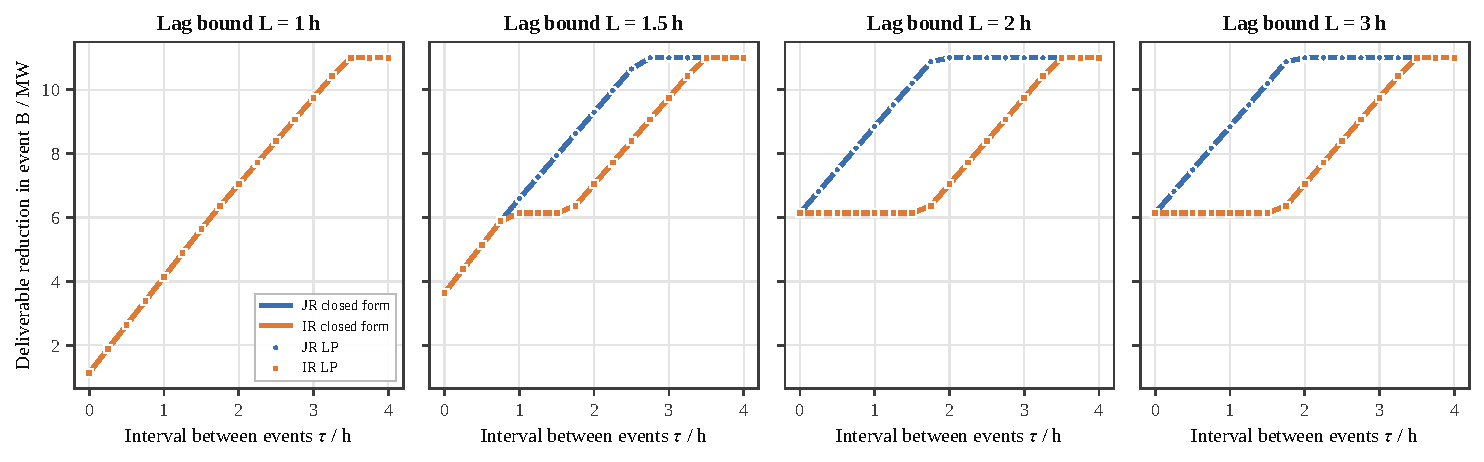
\includegraphics[width=\textwidth]{fig12_stylized_theorem.pdf}
\caption{Numerical check of Theorem~\ref{thm:closed}: closed form (lines) and discrete-time LP (markers) of the
deliverable reduction in event B ($p_f=5$~MW, $D_B=1$~h, $X=5$~MWh, $P_s=6$~MW, $E_A=1.2$~MWh,
$\eta_{\mathrm c}=\eta_{\mathrm d}=0.95$, $h=3$~MW; 68 cases, maximum deviation $10^{-5}$~MW).}
\label{fig:theorem}
\end{figure*}

\paragraph{Proof of Proposition~\ref{prop:price}} All statements are stationarity conditions of the LP with fixed
binaries. For $\Pch_t$, with cost $\cdeg\dt$, coefficient $-1$ in the electricity balance and $-\eta_{\mathrm c}\dt$ in
the energy equation $E_t-E_{t-1}-\eta_{\mathrm c}\dt\Pch_t+\dt\Pdis_t/\eta_{\mathrm d}=0$, a zero reduced cost at an
interior value gives $\cdeg\dt+\lambda_t\dt-\eta_{\mathrm c}\dt\nu_t=0$; discharging is analogous. The variable
$y_{c,t}$ has no own cost and appears in the backlog equation (coefficient $\dt$), the electricity balance
($-(1+a^{\mathrm{aux}})\pdyn$), the cooling balance ($-\theta\pdyn$) and the GPU capacity; with an interior electric
chiller the cooling dual equals $\lambda_t/\COP_t$, and with free GPU capacity its dual is zero, which gives
$\mu_{c,t}=\varepsilon_t\lambda_t$. Stationarity in $\Pg_t$ gives the decomposition of $\lambda_t$, and stationarity in
$B_{c,t}$ gives $\mu_{c,t}=\mu_{c,t+1}+\cjct\dt-\delta_{c,t}$, where the deadline dual $\delta_{c,t}\ge0$ is non-zero only
when the backlog reaches its bound. Combining the conditions yields \eqref{eq:equalmarginal}. $\square$

\paragraph{Proof of Proposition~\ref{prop:dro}} Fix $x$ and write $f_\omega=f_\omega(x)$. With $u_\omega\ge|p_\omega-\hat
p_\omega|$ the inner problem is the LP $\max\sum_\omega f_\omega p_\omega$ subject to $\sum_\omega p_\omega=1$ (dual
$\eta$), $p_\omega-u_\omega\le\hat p_\omega$ ($\alpha_\omega\ge0$), $-p_\omega-u_\omega\le-\hat p_\omega$ ($\beta_\omega\ge0$)
and $\sum_\omega u_\omega\le\delta$ ($\nu\ge0$). Its dual is $\min\eta+\sum_\omega\hat p_\omega(\alpha_\omega-\beta_\omega)+\delta\nu$
subject to $\eta+\alpha_\omega-\beta_\omega\ge f_\omega$ and $\nu\ge\alpha_\omega+\beta_\omega$. With
$\lambda_\omega=\alpha_\omega-\beta_\omega$, the minimum of $\alpha_\omega+\beta_\omega$ is $|\lambda_\omega|$, so the
constraints become $|\lambda_\omega|\le\nu$. The primal is feasible ($p=\hat p$) and bounded, so strong duality holds and
the inner maximum can be replaced by this minimum, which turns \eqref{eq:dro} into a single minimisation with
$f_\omega(x)\le\eta+\lambda_\omega$. Because $f_\omega(x)$ is itself a minimum over $y_\omega$ and the constraint is
monotone in $f_\omega$, ``there is $y_\omega\in\mathcal Y_\omega(x)$ with $c_\omega^\top y_\omega\le\eta+\lambda_\omega$''
is equivalent to $f_\omega(x)\le\eta+\lambda_\omega$, which gives \eqref{eq:droR}. For $\delta=0$, $\nu$ is free and
$\lambda_\omega=f_\omega-\eta$ yields $\sum_\omega\hat p_\omega f_\omega$ (SP); for $\delta\ge2(1-\min_\omega\hat p_\omega)$,
$\mathcal P_\delta$ contains every point mass and the inner maximum is $\max_\omega f_\omega$ (RO). Moving probability
from the cheapest scenarios to the most expensive one is the greedy solution of the inner LP, whose value is concave and
piecewise linear in $\delta$ with slopes $(f_{\bar\omega}-f_\omega)/2$; $V(\delta)$, the infimum of such functions over
$x$, is non-decreasing and concave, and with fixed binaries $\nu^*$ is a supergradient by the envelope theorem.
$\mathrm{CVaR}_\beta$ corresponds to $\{p:0\le p_\omega\le\hat p_\omega/(1-\beta),\sum_\omega p_\omega=1\}$ and is linearised
by $\mathrm{CVaR}_\beta=\min_\eta\eta+\frac1{1-\beta}\sum_\omega\hat p_\omega(f_\omega-\eta)^+$~\cite{rockafellar2000}. $\square$

\paragraph{Proof of Proposition~\ref{prop:region}} (i) Delivering $C$ means that $(C,x)$ satisfies linear constraints:
the joint model, no overdue work, $\Pg_t\le\Pcap$, mean reductions of at least $C_k$, and $C\ge0$. $\Cset$ is the
projection of this polyhedron on $C$ and therefore a convex polyhedron. It is downward closed because a reduction of at
least $C_k$ is also at least $C'_k\le C_k$, contains the origin when non-empty, and $C\in\Cset$ implies
$(0,\dots,C_k,\dots,0)\in\Cset$, hence $C_k\le\Gamma^0_k$, which gives $\Cset\subseteq\mathcal B$ and boundedness. (ii)
The second stage of a sequential strategy is the joint model with the IT plan fixed, so its feasible operations are
feasible for the joint model. (iii) Writing the import as
$\Pg_t=P^{\mathrm{nom}}_t+\varepsilon\sum_c(y_{c,t}-a_{c,t}/\dt)+\Pch_t-\Pdis_t+(\Qtc_t-\Qtd_t)/\COP-\Delta g_t$ (plus PV
curtailment, which only raises the import) and summing over the events of $S$,
$\sum_{k\in S}D_kC_k\le\Delta_S+\varepsilon[\text{backlog increase in the events}]+[\text{net storage discharge in the
events}]+gD_S$. The backlog increase equals $X(e_j)-X(s_i^-)+\sum_{\Iset} C_{\Iset}\le\bar X(e_j)+\sum_{\Iset} C_{\Iset}$ by
Lemma~\ref{lem:edf}; the net discharge is at most $E_s^{\max}+\sum_{\Iset} D_{\Iset}$ because $\phi(x)\le x$; and in every
gap $C_{\Iset}+D_{\Iset}\le\sum_{t\in\Iset}[(\Pcap-P^{\mathrm{nom}}_t)^++g]\dt$. Adding the three inequalities gives
\eqref{eq:multibound}. (iv) Every constraint of $\mathcal T$ is valid for $\Cset$, so $\Cset\subseteq\mathcal T$. For a
vertex $v$, $\theta^*\le\theta_v$, $\theta_vv\in\Cset$ and $0\in\Cset$, so convexity gives $\theta^*v\in\Cset$ and
$\theta^*\mathcal T=\mathrm{conv}\{\theta^*v\}\subseteq\Cset$. (v) The solver's response is one element of the optimal
response set, which gives the first inclusion; the second follows from (ii). Membership in $\Cset_{\mathrm{IR\text{-}P+}}$
is the feasibility of one LP that stacks the joint model for $C$ and the IT model for the price, equates their IT plans
and bounds the IT objective by its optimum plus a tolerance. $\square$

\paragraph{Proof of Proposition~\ref{prop:admm}} (i) Minimising over $x_{\mathrm{IT}}$ for fixed $p$ and over $x_{\mathrm F}$
for fixed $q$ and setting $p=q$ gives the decomposition; LP value functions are convex and piecewise linear in their
right-hand sides ($+\infty$ where infeasible). (ii) $F_{\mathrm{IT}}$ and $F_{\mathrm F}$ are closed proper convex
functions and LP strong duality provides a saddle point of the augmented Lagrangian, which are the conditions of the ADMM
convergence theorem~\cite{boyd2011}; residual, objective and dual convergence are its conclusions. (iii) In the
facility's stationarity condition for $q_t$, which enters the electricity balance with coefficient $-(1+a^{\mathrm{aux}})$
and the cooling balance with $-\theta$, the electricity dual is $\dt\lch_t$ and, with an interior chiller, the cooling
dual $\dt\lch_t/\COP_t$, hence $\lambda^*_t=\dt\lch_t(1+a^{\mathrm{aux}}+\theta/\COP_t)$. (iv) The proximal terms are
strictly convex in $p$ and $q$. $\square$

In the implementation, the unscaled form \eqref{eq:admm} is essential. In the scaled form
$\frac{\rho}{2}\|p-q^k+\lambda^k/\rho\|^2$, the deviation at convergence is about $\lambda/\rho$, which falls where
the tangent points are sparse; the jumps of the subgradient at the kinks then act as price errors of several hundred
CNY per MW and step, and the iteration stalls at a suboptimal point (2.1\% above the optimum for $\rho=800$). The two
forms are equivalent in exact arithmetic. The open-loop and closed-loop checks are reported in \secref{sec:res-admm}.

\section{Supplementary results and reproducibility}
\label{app:supp}
\appendixnumbering

\figref{fig:mcbox} shows the box plots of fulfilment and total cost on the 52 operating days that underlie
\tabref{tab:mc}, and \figref{fig:sens0} repeats the sensitivity study of \figref{fig:sens} in the rule setting.
\tabref{tab:repro} lists, for every experiment, the script and the result files from which the tables and figures of this
paper are generated. All experiments run with GNU Octave 8.4 and glpk (or MATLAB with intlinprog or Gurobi through the
same interface); the complete set takes about 18~h in a single process or about 3~h in parallel batches, and the
smoke tests check that every optional feature leaves the base case unchanged when it is switched off.

\begin{figure*}[!t]
\centering
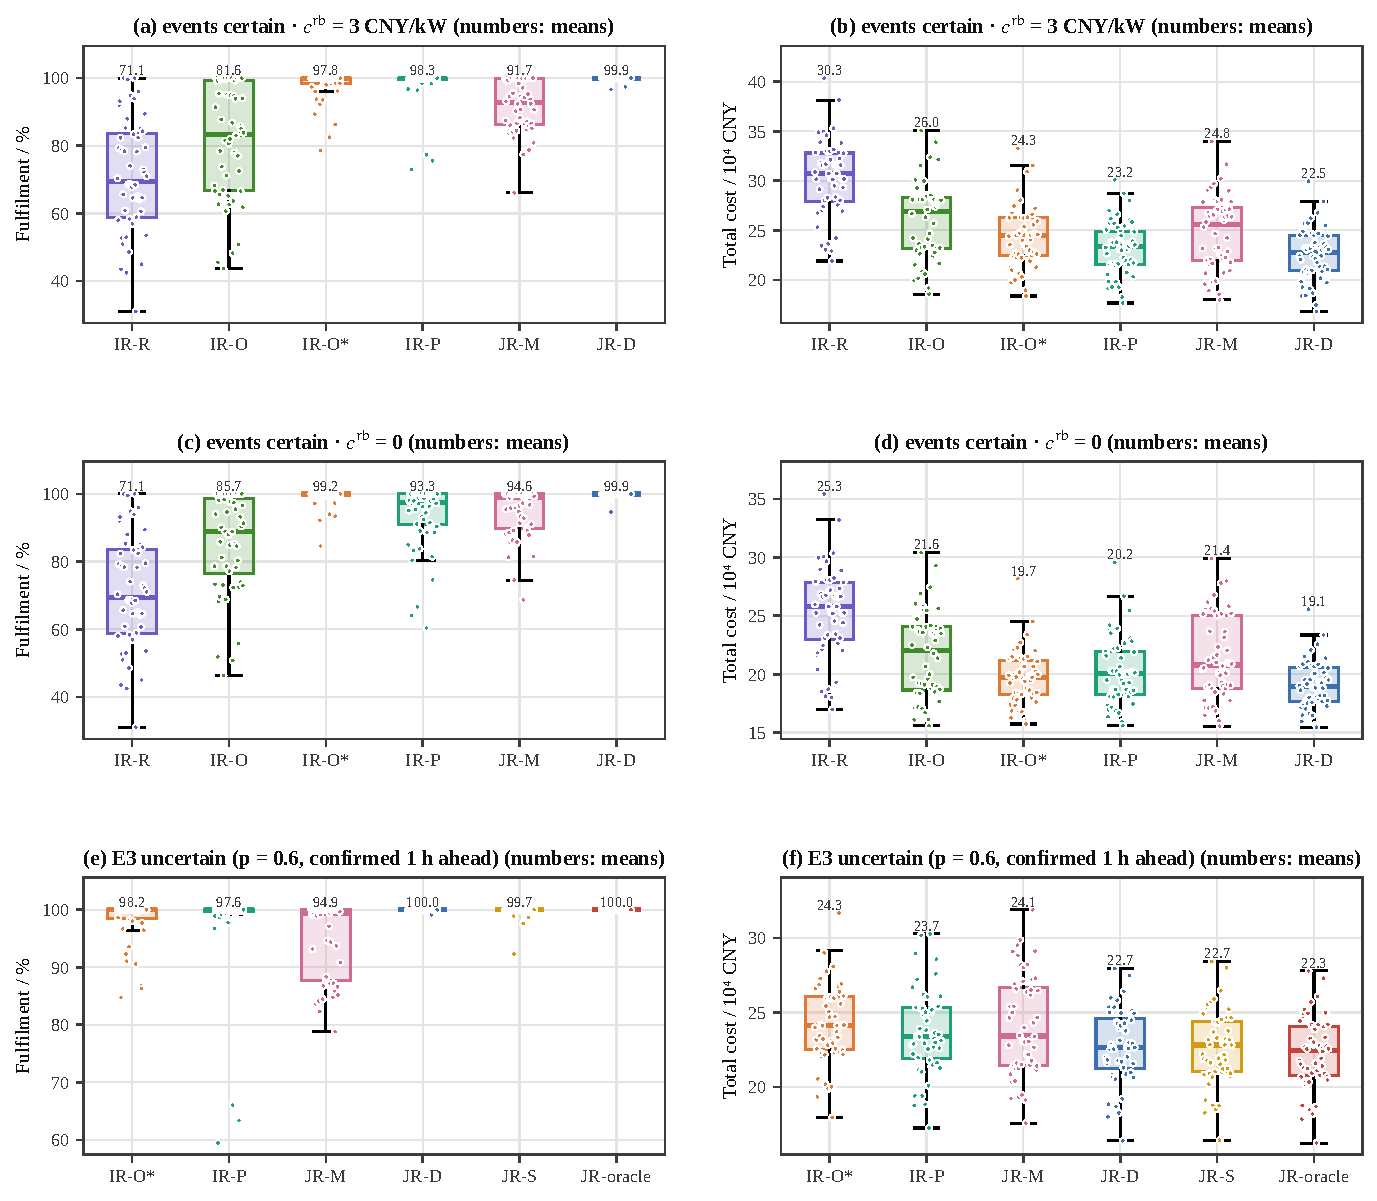
\includegraphics[width=0.86\textwidth]{fig07_montecarlo.pdf}
\caption{Fulfilment and total cost on the 52 operating days for the three settings (numbers: means).}
\label{fig:mcbox}
\end{figure*}

\begin{figure*}[!t]
\centering
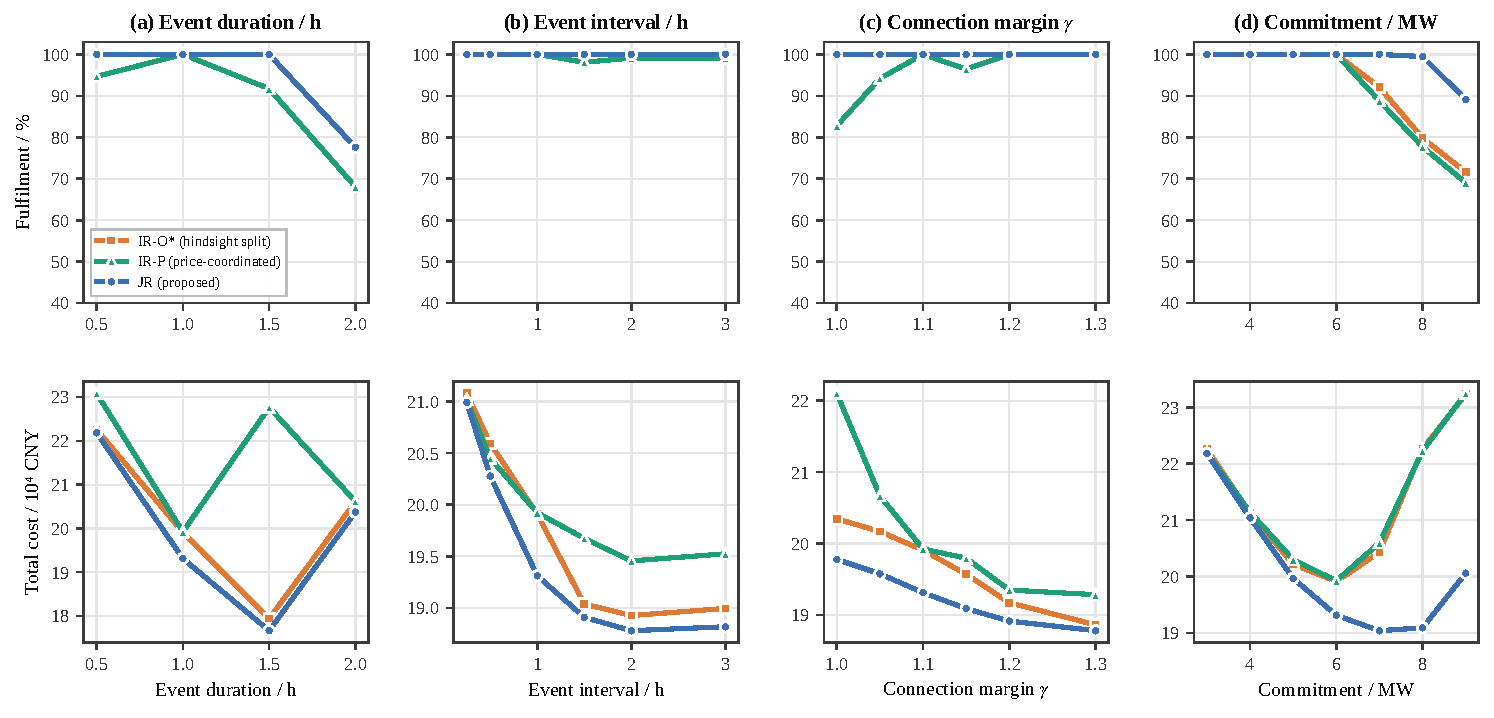
\includegraphics[width=0.96\textwidth]{fig05_sensitivity_crb0.pdf}
\caption{Sensitivity under perfect information in the rule setting ($\crb=0$): fulfilment (top) and total cost (bottom)
versus (a) event duration, (b) gap, (c) connection margin and (d) uniform commitment.}
\label{fig:sens0}
\end{figure*}

\begin{table*}[!t]
\caption{Experiments, scripts and result files (scripts in \texttt{matlab/experiments}, results in \texttt{matlab/results}).}
\label{tab:repro}
\centering\scriptsize
\setlength{\tabcolsep}{4pt}
\begin{tabularx}{\textwidth}{@{}c>{\raggedright\arraybackslash}p{0.16\textwidth}>{\raggedright\arraybackslash}p{0.19\textwidth}X@{}}
\toprule
No. & Experiment & Script & Result files\\
\midrule
1 & Mechanism & \texttt{exp1\_mechanism.m} & \texttt{exp1\_mechanism\_CA6\_DA2}, \texttt{exp1\_mechanism\_CA6\_DA1\_DB2}\\
2 & Case day & \texttt{exp2\_main.m} & \texttt{exp2\_\{DAcommit,uniform6\}[\_crb0]}, \texttt{exp2\_commitments}, \texttt{exp2\_alpha\_*}, \texttt{exp2\_lambda\_*}, \texttt{ts\_*}\\
3 & Sensitivity & \texttt{exp3\_sensitivity.m} & \texttt{exp3\_\{duration,interval,gamma,commitment,map\}[\_crb0]}\\
4 & 52 operating days & \texttt{exp4\_montecarlo.m} & \texttt{exp4\_\{certain,certain\_crb0,e3uncertain\}} with \texttt{\_strategies}, \texttt{\_bench}\\
5 & Shadow prices & \texttt{exp5\_shadow.m} & \texttt{exp5\_shadow*}, \texttt{exp5\_kkt*} (KKT residuals)\\
6 & Commitment pairing & \texttt{exp6\_commitment.m} & \texttt{exp6\_commitment[\_crb0]}, \texttt{exp6\_theta[\_crb0]}\\
7 & Ablation & \texttt{exp7\_ablation.m} & \texttt{exp7\_ablation}, \texttt{exp7\_alpha}\\
8 & Rebound charge & \texttt{exp8\_rebound.m} & \texttt{exp8\_rebound}, \texttt{exp8\_strategies}\\
9 & Payment $\times$ shortfall & \texttt{exp9\_price.m} & \texttt{exp9\_price}, \texttt{exp9\_strategies}\\
10 & Realism & \texttt{exp10\_realism.m} & \texttt{exp10\_realism}\\
11 & Theorem 1 & \texttt{exp11\_stylized.m} & \texttt{exp11\_stylized}\\
12 & Reliable capacity & \texttt{exp12\_capacity.m} & \texttt{exp12\_capacity\_crb0}, \texttt{exp12\_strategies\_crb0}\\
13 & Substitution & \texttt{exp13\_substitution.m} & \texttt{exp13\_substitution}, \texttt{exp13\_strategies}\\
14 & Timing & \texttt{exp14\_timing.m} & \texttt{exp14\_timing}\\
15 & Risk-averse commitment & \texttt{exp15\_risk.m} & \texttt{exp15\_commit}, \texttt{exp15\_oos}, \texttt{exp15\_settings}\\
16 & Tariff shapes & \texttt{exp16\_tariff.m} & \texttt{exp16\_tariff}, \texttt{exp16\_tariff\_mc}, \texttt{exp16\_shapes}\\
17 & Policy and coupling & \texttt{exp17\_policy.m} & \texttt{exp17\_policy}, \texttt{exp17\_strategies}\\
18 & Climate & \texttt{exp18\_climate.m} & \texttt{exp18\_climate}, \texttt{exp18\_climate\_mc}, \texttt{exp18\_cases}\\
19 & Job-level validation & \texttt{exp19\_workload.m} & \texttt{exp19\_workload\_\{pai,acme\}\_\{fluid,rigid\}}, \texttt{exp19\_variants}, \texttt{ts\_job\_*}\\
20 & Job mix and overheads & \texttt{exp20\_jobsim.m} & \texttt{exp20\_jobsim}, \texttt{exp20\_settings}, \texttt{exp20\_strategies}\\
21 & Offshore wind & \texttt{exp21\_wind.m} & \texttt{exp21\_curve}, \texttt{exp21\_wind}, \texttt{exp21\_strategies}\\
22 & Overheads and capping & \texttt{exp22\_overhead.m} & \texttt{exp22\_overhead\_\{a,b,c\}}, \texttt{exp22\_settings}\\
23 & Scenario generation & \texttt{exp23\_scenarios.m} & \texttt{exp23\_commit}, \texttt{exp23\_oos}, \texttt{exp23\_settings}\\
24 & Waste-heat recovery & \texttt{exp24\_heat.m} & \texttt{exp24\_heat}, \texttt{exp24\_settings}, \texttt{ts\_heat\_*}\\
25 & Capability region & \texttt{exp25\_region.m} & \texttt{exp25\_\{case,radial,vertices,irp,slices,sweep,mc,irp\_eps\}}\\
26 & Distributed coordination & \texttt{exp26\_admm.m} & \texttt{exp26\_\{conv,ref,price\}}, \texttt{exp26\_mc}, \texttt{exp26\_rho}, \texttt{exp26\_strategies}\\
\bottomrule
\end{tabularx}
\end{table*}


\section*{Data availability}
All inputs are public: the Alibaba PAI GPU cluster trace~\cite{weng2022}, the Azure LLM inference trace~\cite{stojkovic2025},
the Acme LLM development trace (CC BY 4.0)~\cite{hu2024acme}, ERA5 weather and wind data~\cite{hersbach2020} retrieved
from Open-Meteo, the Jiangsu TOU tariff and the Jiangsu DR rules~\cite{jiangsu2024dr}. The MATLAB/GNU Octave code and the
processed data that reproduce all 26 experiments, figures and tables will be made openly available upon publication.

% generated by tools/order_refs.py -- do not edit; edit references.tex instead
\begin{thebibliography}{99}
\bibitem{iea2025} International Energy Agency. Energy and AI. Paris: IEA; 2025.
\bibitem{shehabi2024} Shehabi A, Smith SJ, Hubbard A, et al. 2024 United States data center energy usage report. Berkeley, CA: Lawrence Berkeley National Laboratory; 2024.
\bibitem{ndrc2024dc} National Development and Reform Commission, Ministry of Industry and Information Technology, National Energy Administration, National Data Administration. Special action plan for the green and low-carbon development of data centers. Beijing; 2024 [in Chinese].
\bibitem{norris2025} Norris TH, Profeta T, Pati\~no-Echeverri D, Cowie-Haskell A. Rethinking load growth: assessing the potential for integration of large flexible loads in US power systems. Durham, NC: Nicholas Institute for Energy, Environment \& Sustainability, Duke University; 2025.
\bibitem{chen2026defer} Chen Y, Zheng X. To defer or to shift? The role of AI data center flexibility on grid interconnection. arXiv:2604.05376; 2026.
\bibitem{texas2025sb6} Texas Legislature. Senate Bill 6, 89th Legislature: interconnection and curtailment of large loads. Austin, TX; 2025.
\bibitem{williams2026} Williams C, Colangelo P, Coskun AK, et al. Power-flexible AI data centers: a new paradigm for grid-responsive compute. arXiv:2606.25098; 2026.
\bibitem{colangelo2025} Colangelo P, Coskun AK, Megrue J, et al. Turning AI data centers into grid-interactive assets: results from a field demonstration in Phoenix, Arizona. arXiv:2507.00909; 2025.
\bibitem{ndrc2023dsm} National Development and Reform Commission, et al. Measures for the administration of power demand-side management (2023 edition). Beijing; 2023 [in Chinese].
\bibitem{jiangsu2024dr} Jiangsu Provincial Development and Reform Commission. Implementation rules for power demand response in Jiangsu Province. Nanjing; 2024 [in Chinese].
\bibitem{liu2013} Liu Z, Wierman A, Chen Y, Razon B, Chen N. Data center demand response: avoiding the coincident peak via workload shifting and local generation. Perform Eval 2013;70(10):770--91.
\bibitem{wierman2014} Wierman A, Liu Z, Liu I, Mohsenian-Rad H. Opportunities and challenges for data center demand response. In: Proceedings of the International Green Computing Conference (IGCC); 2014.
\bibitem{chen2020review} Chen M, Gao C, Song M, et al. Internet data centers participating in demand response: a comprehensive review. Renew Sustain Energy Rev 2020;117:109466.
\bibitem{radovanovic2023} Radovanovi\'c A, Koningstein R, Schneider I, et al. Carbon-aware computing for datacenters. IEEE Trans Power Syst 2023;38(2):1270--80.
\bibitem{acun2026} Acun F, Hankendi C, Levine E, Reynolds H, Bardwick J, Coskun AK. Investigating power consumption flexibility of AI data centers for demand response participation. In: Proceedings of the ACM International Conference on Future and Sustainable Energy Systems (e-Energy); 2026.
\bibitem{patel2024} Patel P, Choukse E, Zhang C, et al. Characterizing power management opportunities for LLMs in the cloud. In: Proceedings of the ACM International Conference on Architectural Support for Programming Languages and Operating Systems (ASPLOS); 2024, p. 207--22.
\bibitem{du2026} Du B, Fan X, Du E, Chen L, Han J, Hou Q, et al. From tokens to energy flexibility: quantization-enabled demand response for data centers with LLM inference workloads. arXiv:2606.18851; 2026.
\bibitem{google2025} Google. Demand response agreements with Indiana Michigan Power and the Tennessee Valley Authority for machine-learning workloads. Company announcement, 4 August 2025.
\bibitem{li2026scalar} Li M. Beyond scalar flexibility: from eligible AI workloads to dependable load relief. arXiv:2609.05406; 2026.
\bibitem{choukse2025} Choukse E, et al. Power stabilization for AI training datacenters. arXiv:2508.14318; 2025.
\bibitem{han2024} Han O, Ding T, Yang M, et al. A novel 4-level joint optimal dispatch for demand response of data centers with district autonomy realization. Appl Energy 2024;358:122590.
\bibitem{lin2025} Lin J, Han J, Wang Y, et al. Planning and operation optimization of a computing-power integrated energy system for low-carbon data centers considering exergy efficiency. J Shanghai Jiao Tong Univ 2025;59(9):1327--37 [in Chinese].
\bibitem{fan2026} Fan H, Chen S, Luo H, et al. Optimal operation strategy of data centers considering cooling--heating--power multi-energy complementarity and spatio-temporally adjustable loads. South Power Syst Technol 2026;20(5):28--36 [in Chinese].
\bibitem{zhang2026bilevel} Zhang S, Ding S, Li Y, Wei M, Tan Q. A bi-level planning model of integrated energy capacity configuration for data center cluster considering computing-electricity coupling operation and supply-demand uncertainties. Appl Energy 2026;425:128499.
\bibitem{huang2020} Huang P, Copertaro B, Zhang X, et al. A review of data centers as prosumers in district energy systems: renewable energy integration and waste heat reuse for district heating. Appl Energy 2020;258:114109.
\bibitem{wahlroos2018} Wahlroos M, P\"arssinen M, Rinne S, et al. Future views on waste heat utilization -- case of data centers in Northern Europe. Renew Sustain Energy Rev 2018;82(2):1749--64.
\bibitem{evans2022} Evans MP, Tindemans SH, Angeli D. Flexibility framework with recovery guarantees for aggregated energy storage devices. IEEE Trans Smart Grid 2022;13(5):3519--31.
\bibitem{hao2015} Hao H, Sanandaji BM, Poolla K, Vincent TL. Aggregate flexibility of thermostatically controlled loads. IEEE Trans Power Syst 2015;30(1):189--98.
\bibitem{wrinch2012} Wrinch M, Dennis G, El-Fouly THM, Wong S. Demand response implementation for improved system efficiency in remote communities. In: Proceedings of the IEEE Electrical Power and Energy Conference (EPEC); 2012.
\bibitem{chao2011} Chao H. Demand response in wholesale electricity markets: the choice of customer baseline. J Regul Econ 2011;39(1):68--88.
\bibitem{schildbach2014} Schildbach G, Fagiano L, Frei C, Morari M. The scenario approach for stochastic model predictive control with bounds on closed-loop constraint violations. Automatica 2014;50(12):3009--18.
\bibitem{zeng2013} Zeng B, Zhao L. Solving two-stage robust optimization problems using a column-and-constraint generation method. Oper Res Lett 2013;41(5):457--61.
\bibitem{esfahani2018} Mohajerin Esfahani P, Kuhn D. Data-driven distributionally robust optimization using the Wasserstein metric: performance guarantees and tractable reformulations. Math Program 2018;171(1--2):115--66.
\bibitem{boyd2011} Boyd S, Parikh N, Chu E, Peleato B, Eckstein J. Distributed optimization and statistical learning via the alternating direction method of multipliers. Found Trends Mach Learn 2011;3(1):1--122.
\bibitem{stojkovic2025} Stojkovic J, Zhang C, Goiri \'I, Torrellas J, Choukse E. DynamoLLM: designing LLM inference clusters for performance and energy efficiency. In: Proceedings of the IEEE International Symposium on High-Performance Computer Architecture (HPCA); 2025.
\bibitem{weng2022} Weng Q, Xiao W, Yu Y, et al. MLaaS in the wild: workload analysis and scheduling in large-scale heterogeneous GPU clusters. In: Proceedings of the 19th USENIX Symposium on Networked Systems Design and Implementation (NSDI); 2022.
\bibitem{fan2007} Fan X, Weber W-D, Barroso LA. Power provisioning for a warehouse-sized computer. In: Proceedings of the 34th Annual International Symposium on Computer Architecture (ISCA); 2007, p. 13--23.
\bibitem{hu2024acme} Hu Q, Ye Z, Wang Z, et al. Characterization of large language model development in the datacenter. In: Proceedings of the 21st USENIX Symposium on Networked Systems Design and Implementation (NSDI); 2024.
\bibitem{ashrae2021} ASHRAE Technical Committee 9.9. Thermal guidelines for data processing environments. 5th ed. Atlanta, GA: ASHRAE; 2021.
\bibitem{ndrc2025green} National Development and Reform Commission, National Energy Administration. Notice on promoting green-power direct connection in an orderly manner (Fagai Nengyuan [2025] No. 650). Beijing; 2025 [in Chinese].
\bibitem{hersbach2020} Hersbach H, Bell B, Berrisford P, et al. The ERA5 global reanalysis. Q J R Meteorol Soc 2020;146(730):1999--2049.
\bibitem{gaertner2020} Gaertner E, Rinker J, Sethuraman L, et al. Definition of the IEA 15-megawatt offshore reference wind turbine. Golden, CO: National Renewable Energy Laboratory; 2020. Report NREL/TP-5000-75698.
\bibitem{meta2018odense} Meta. Odense data center: heat recovery to the Fjernvarme Fyn district heating network. Company information; 2018.
\bibitem{ndrc2016demand} General Office of the National Development and Reform Commission. Notice on improving the implementation of the basic electricity price for two-part tariff users (Fagai Ban Jiage [2016] No. 1583). Beijing; 2016 [in Chinese].
\bibitem{mee2024ef} Ministry of Ecology and Environment, National Bureau of Statistics. Announcement on the 2022 carbon dioxide emission factors of electricity. Beijing; 2024 [in Chinese].
\bibitem{rockafellar2000} Rockafellar RT, Uryasev S. Optimization of conditional value-at-risk. J Risk 2000;2(3):21--41.
\bibitem{latif2024} Latif I, Newkirk AC, Carbone MR, et al. Empirical measurements of AI training power demand on a GPU-accelerated node. arXiv:2412.08602; 2024.
\bibitem{xu2018} Xu B, Zhao J, Zheng T, Litvinov E, Kirschen DS. Factoring the cycle aging cost of batteries participating in electricity markets. IEEE Trans Power Syst 2018;33(2):2248--59.
\bibitem{dobos2014} Dobos AP. PVWatts version 5 manual. Golden, CO: National Renewable Energy Laboratory; 2014. Report NREL/TP-6A20-62641.
\bibitem{wan2025} Wan B, Han M, Sheng Y, et al. ByteCheckpoint: a unified checkpointing system for large foundation model development. In: Proceedings of the 22nd USENIX Symposium on Networked Systems Design and Implementation (NSDI); 2025.
\bibitem{wang2023gemini} Wang Z, Jia Z, Zheng S, et al. Gemini: fast failure recovery in distributed training with in-memory checkpoints. In: Proceedings of the 29th ACM Symposium on Operating Systems Principles (SOSP); 2023.
\end{thebibliography}

\end{document}
